% ============================================================================
%  ACCORD thesis -- master document
%
%  Build:  pdflatex main && bibtex main && pdflatex main && pdflatex main
%     or:  ./build.sh
%
%  Chapters are \input files with no preamble of their own; every package a
%  chapter depends on is loaded here. The chapter headers each name their
%  requirements (booktabs, amsmath, graphicx, natbib) -- that list is the
%  contract this file satisfies.
%
%  Figures: the 14 figure environments in the chapters are written as
%  specifications rather than \includegraphics calls. \figspec renders a
%  visible placeholder box carrying the spec text, so the document compiles
%  and every unrendered figure is obvious in the PDF rather than silently
%  missing. Replace with \includegraphics as assets are produced.
% ============================================================================

\documentclass[11pt,oneside]{book}

\usepackage[utf8]{inputenc}
\usepackage[T1]{fontenc}
\usepackage[margin=1.25in]{geometry}
\usepackage{booktabs}
\usepackage{amsmath}
\usepackage{amssymb}
\usepackage{graphicx}
\usepackage{longtable}
\usepackage{array}
\usepackage{multirow}
\usepackage{xcolor}
\usepackage[round]{natbib}
\usepackage[hidelinks]{hyperref}
\usepackage{microtype}

% Placeholder for figures that exist as written specs, not assets.
\newcommand{\figspec}[1]{%
  \begin{center}
  \fcolorbox{black!40}{black!5}{%
    \parbox{0.9\linewidth}{\vspace{0.5em}\small\textbf{[FIGURE SPEC --- asset not yet rendered]}\\[0.3em]#1\vspace{0.5em}}}
  \end{center}}

\title{Why Clinical NLP Pipelines Are Evaluated With Instruments That Do Not Measure What They Are Believed To Measure}
\author{Ricky Gole}
\date{\today}

\begin{document}

\frontmatter
\maketitle

\chapter*{Abstract}
\addcontentsline{toc}{chapter}{Abstract}

[TODO: abstract. Draft after the chapter reorganization settles. It must not
overclaim: the evaluation cannot establish that the task is unsolvable (minimum
detectable AUROC $0.7382$ at $80\%$ power with twelve positives), no subgroup
harm is demonstrated, and neither proposed architecture survived its own
control. What it can claim is the demonstration itself --- nine instruments,
two systems, each checked against a control that cost hours and was not run.]

\tableofcontents
\listoftables

\mainmatter

% ============================================================================
%  Chapter 1. Introduction
%
%  \input file. No preamble. The parent document must load:
%      \usepackage{booktabs}   % \toprule \midrule \bottomrule \cmidrule
%      \usepackage{amsmath}    % aligned display math
%      \usepackage{graphicx}   % (only if figure assets are substituted in)
%      \usepackage[round]{natbib}  % \citep \citet
%  Bibliography: accord/thesis/refs.bib
%
%  Every quantity in this chapter is forward-referenced to the chapter that
%  derives it. No number appears here that is not derived in Chapters 3 to 8 or
%  recorded in accord/CORRECTIONS.md.
% ============================================================================

\chapter{Introduction}
\label{ch:intro}

\section{A Patient Goes Home on a Held Medication}
\label{sec:intro-problem}

A patient admitted for decompensated heart failure is discharged on eleven
medications. Somewhere in the middle of the stay a nurse records that the loop
diuretic was withheld because the patient had become hypovolemic. Two days
later the discharge summary, written by a physician who is reconciling a
medication list against an admission list, instructs that the same diuretic be
continued at its admission dose. The two documents disagree. Only one of them
governs what the patient does after leaving the building, and it is not the one
that contains the reason the instruction is wrong.

Nothing about this scenario is exotic. Polypharmacy is the norm in heart
failure, the drugs involved have narrow therapeutic windows, and the transition
from inpatient to outpatient care is the single most error-prone moment in the
medication lifecycle. Unintended medication discrepancies are present in a
large share of hospital admissions \citep{cornish2005discrepancies} and
discharges \citep{wong2008reconciliation}; adverse events in the weeks after
discharge are common, frequently drug-related, and frequently preventable
\citep{forster2003adverse}; errors traceable to discontinuity between the
inpatient and outpatient settings affect a substantial fraction of discharged
patients \citep{moore2003discontinuity}; and the information transfer that
would prevent them is unreliable in both content and timing
\citep{kripalani2007deficits}. Adverse drug events were established as a
first-order inpatient safety problem three decades ago
\citep{bates1995ade} and the transition-of-care component of that problem has
not been solved since.

This thesis takes as its object one narrow, checkable instance of that problem:
a \emph{cross-note medication contradiction}, defined as a disagreement about a
specific drug between a nursing progress note and the discharge summary of the
same admission. Chapter~\ref{ch:candidates} constructs four transparent rules
over extracted medication mentions and applies them to MIMIC-III
\citep{johnson2016mimic}, yielding $1{,}978$ candidate contradictions across
$1{,}203$ admissions drawn from a heart-failure cohort of $9{,}783$. A
board-certified pharmacist annotating a stratified sample of those candidates
confirmed $12$ genuine contradictions in $299$ pairs, four of them rated $4$ or
$5$ on a five-point danger scale.

Those numbers establish the tension this thesis is built on. The phenomenon is
systematic rather than anecdotal: rules over a single institution's notes
surface nearly two thousand candidates, and a domain expert confirms that some
of them are real and dangerous. But the phenomenon is also \emph{rare} in the
population a system would have to screen, and rarity is not a nuisance
parameter here. It is the thing that breaks every stage of the pipeline that
follows.

\section{The Pipeline the Field Would Build, and Where It Breaks}
\label{sec:intro-gap}

Faced with this problem, the standard construction is close to automatic. Mine
candidates with cheap, high-recall rules, because exhaustive expert review of
every cross-note medication pair is infeasible. Label the candidates with an
instruction-tuned language model, because expert annotation does not scale and
recent work reports that such models match or exceed crowd annotators on many
classification tasks \citep{gilardi2023chatgpt}. Distil those labels into a
purpose-built neural detector over a domain-pretrained clinical encoder
\citep{gu2021biomedbert,alsentzer2019clinicalbert}, with architectural
components encoding the domain structure that generic natural language
inference models lack. Evaluate against the expert annotations. Report.

The construction is defensible at every step, and this thesis executed it. It
fails at every step, and the failures are not the ones the literature would
predict.

\paragraph{The gap.} Prior work on clinical natural language inference
establishes that encoder models can classify entailment relations between
clinician-authored sentence pairs \citep{romanov2018mednli}, and prior work on
weak supervision establishes that noisy programmatic labels can substitute for
hand annotation when the noise sources are multiple and their errors are
conditionally independent \citep{ratner2016dataprogramming,ratner2017snorkel}.
Neither body of work addresses what happens when the positive class occupies
four percent of an already-enriched candidate pool, when there is exactly one
noise source, and when that source's error is a systematic prior shift rather
than independent noise. Under those conditions the standard recipe does not
degrade gracefully. It produces a system whose outputs are statistically
independent of the labels, and it produces that system while emitting metrics
that look survivable.

\paragraph{The consequence for what gets reported.} The reason this matters
beyond one project is that the failure is quiet. A system with no signal, trained
on supervision whose marginal is inverted, still produces a contradiction
$F_1$, a recall figure, an ablation table, and an auxiliary-task accuracy. Every
one of those numbers can be reported in good faith by someone who has not run
the specific diagnostic that would falsify it. Chapters~\ref{ch:arch}
and~\ref{ch:eval} document four such claims from this project's own earlier
submission, each of which survived internal review and none of which survives
its own first check.

\section{Research Questions}
\label{sec:intro-rqs}

The project was designed around four questions. They are stated here in the
form in which they were posed, before the answers were known, because the value
of the thesis lies substantially in the gap between what was asked and what
turned out to be answerable.

\begin{description}
\item[RQ1 (Authority).] Does conditioning a cross-note inference model on
      \emph{note-type authority} outperform symmetric natural language
      inference? The construct, developed in Chapter~\ref{ch:data} as
      \emph{clinical note priority}, is that a discharge summary and a nursing
      progress note carry different institutional weight, so a disagreement
      between them is not a symmetric relation.
\item[RQ2 (Temporality).] Does encoding temporal metadata, the ordering of the
      two notes and the interval between them, improve detection over a
      time-agnostic pairwise model?
\item[RQ3 (Severity).] Can published clinical practice guidelines be used to
      rank confirmed contradictions by danger, so that a triage system surfaces
      the harmful ones first?
\item[RQ4 (Supervision).] Can weak supervision from an instruction-tuned
      language model replace expert annotation at the scale required to train a
      detector for a rare clinical event?
\end{description}

\section{Contributions, Stated as Findings}
\label{sec:intro-contributions}

This thesis contributes no working system. Its contributions are measurements,
and they are stated as such. Each is a finding about the pipeline rather than a
component of it, each is traceable to a named chapter, and each is accompanied
by the diagnostic that would have produced it earlier.

\begin{enumerate}
\item \textbf{Rule-based candidate mining yields a four percent precision pool,
      and the evidence attached to those candidates was frequently the wrong
      evidence.} Four transparent rules enrich the candidate space to a
      pharmacist-measured base rate of $4.0\%$, which is a real and useful
      enrichment over an unfiltered background rate orders of magnitude lower.
      But the mechanism that decided \emph{which} candidate a sentence pair was
      flagged for was independent of the mechanism that selected the sentence
      pair to display, and for $41.4\%$ of action-conflict candidates the
      displayed evidence did not contain the flagged conflict. Every downstream
      consumer, the annotator, the weak labeller, and the model, reasoned about
      that evidence. The $4.0\%$ figure is therefore an upper bound on the
      validity of the annotation exercise rather than a clean estimate of pool
      precision. Chapter~\ref{ch:candidates}.

\item \textbf{Language model weak supervision is miscalibrated by a factor of
      roughly twenty-one, and the detector inherits the labeller's prior rather
      than its judgement.} The weak labeller assigned the positive class to
      $84.9\%$ of $1{,}679$ candidates against a measured base rate of $4.0\%$.
      Under that base rate at least $95\%$ of its positive labels are wrong. The
      trained detector then reproduced the labeller's per-rule
      predicted-positive rate to within $1.5$ percentage points on three of four
      rules, while the rules' true prevalences differ from one another by more
      than a factor of four. Reproducing the quantity that carries no
      information about the truth, and not the quantity that does, is the
      signature of a model that has learned the label's marginal rather than its
      conditional. This answers RQ4 in the negative, and the negative is
      specific: the failure is calibration, not comprehension, because the same
      labeller recovers $11$ of the $12$ true contradictions.
      Chapter~\ref{ch:weak}.

\item \textbf{Authority conditioning contributes nothing, and the claim that it
      does is falsified four independent ways.} The authority parameter reported
      as \emph{discovered} at $(\alpha_N, \alpha_D) \approx (0.5, 1.0)$ was
      \emph{initialised} at exactly $[0.5, 1.0]$; it moved by $1.8\%$ and
      $0.6\%$, agreeing to the third decimal across seeds; it sits on a branch
      that a subsequent LayerNorm largely erases, leaving a near-zero gradient;
      and the project's own ablation shows that constraining
      $\alpha_N = \alpha_D$ \emph{improves} both reported metrics. RQ1 is
      therefore not answered in the affirmative and, more precisely, was never
      tested: the implementation could not have detected an authority signal had
      one existed. Chapter~\ref{ch:arch}.

\item \textbf{The trained detector carries no rank signal, and the finding
      survives the one defect that could plausibly have manufactured it.} On the
      $299$ annotated pairs the contradiction probability achieves AUROC
      $0.460$, average precision at the no-skill line, Mann-Whitney $p = 0.64$,
      and a bootstrap $95\%$ confidence interval of $[0.287, 0.633]$. The
      fifteen highest-scored pairs contain zero true contradictions. Restricted
      to Rules 3 and 4, the strata that are free of the exemplar defect by
      construction, AUROC is $0.5078$ with Mann-Whitney $p = 0.953$, which is
      chance to four significant figures. That stratum contains six positives,
      so the estimate is wide, and it is reported with that width attached.
      Chapters~\ref{ch:eval} and~\ref{ch:discussion}.

\item \textbf{RQ3 is untestable from this work, because the component that would
      have answered it was never trained.} The guideline-grounded harm estimator
      has no guideline corpus; its ``guideline bank'' is twenty randomly
      initialised vectors. Its harm head appears in no term of the training
      objective. Its outputs across the evaluation set span $0.398$ to $0.610$,
      the range of an untrained sigmoid, and correlate with the pharmacist's
      danger rating at $\rho = -0.0001$. That null is a measurement of an
      untrained module, not evidence about whether clinical severity is
      predictable, and reporting it as the latter would be the single most
      misleading move available in this document. Chapters~\ref{ch:arch}
      and~\ref{ch:eval}.

\item \textbf{A prescriptive result about evaluation under low prevalence.} At
      the evaluation set's operating prevalence of $12$ positives against $241$
      negatives, balanced accuracy, Matthews correlation, and
      prevalence-adjusted bias-adjusted kappa all prefer a system that recovers
      $6$ of $12$ contradictions over one that recovers $11$, and the exchange
      rate is available in closed form: the preference flips once the additional
      true negatives per forgone true positive exceed $Q/P = 20.08$.
      Chapter~\ref{ch:metrics} derives this, and then sharpens it against the
      empirical situation, in which the systems being compared mostly have no
      discriminative ability at all.
\end{enumerate}

\paragraph{RQ2 has no answer, for a reason that is itself a finding.}
\texttt{CHARTTIME} is null for $100\%$ of MIMIC-III discharge summaries. The
temporal ordering RQ2 requires cannot be established at finer than day
granularity between the two notes of a pair, and the filter that purported to
measure whether conflicts were resolved by intervening documentation was, on
inspection, matching a twenty-way alternation containing both directions of the
medication decision at once. The temporal question is not answered negatively.
It is unaddressable in this resource, and the correct report is the data
limitation rather than the measurement. Chapter~\ref{ch:data},
Section~\ref{sec:charttime}.

\section{What the Results Look Like}
\label{sec:intro-results}

The headline is stated once, plainly, so that nothing later in the document
reads as a reveal.

On the $299$ pharmacist-annotated pairs, the trained detector predicts
\emph{contradiction} for $278$, achieving precision $0.047$ against a base rate
of $0.040$, recall $0.917$, and accuracy $0.115$. At thresholds of $0.05$,
$0.10$, and $0.15$ it predicts positive for every pair, because no score in the
evaluation set falls below $0.15$. Its Matthews correlation is $-0.007$. The
weak labeller it was distilled from scores $-0.044$, which is worse than
chance. A general-purpose model prompted zero-shot on the same $299$ pairs, with
no training data and no clinical components, is the only system in the
comparison with a positive Matthews correlation, at $+0.109$ and $8.45\%$
precision.

Two consequences follow immediately and are developed at length later. First,
the task is not impossible: something above chance is extractable from the same
evidence, so the failure is a property of this pipeline rather than of the
problem. Second, the failures are causally independent of one another. The
exemplar defect, the prevalence mismatch, the initialisation artifact, the
auxiliary-head leakage, and the untrained severity head each have their own
mechanism and their own detector, and repairing any one of them in isolation
would still leave a system with AUROC near $0.5$.

A third consequence is the one this thesis regards as most transferable. The
component sanity check in Chapter~\ref{ch:eval} shows that BioMedBERT
fine-tuned on MedNLI reaches $83.90\%$ accuracy and $83.91\%$ macro $F_1$,
inside the published range for comparable encoder systems. That result is a
property of the backbone and contains zero components of the system under
study. Reporting it under the system's name would have produced a document in
which a strong number and a failing system coexist without the reader being
able to tell which is which. This thesis does not do that, and
Chapter~\ref{ch:eval} explains why the temptation to do it is structural rather
than personal.

\section{Scope, and What This Thesis Does Not Claim}
\label{sec:intro-scope}

Three boundaries are worth fixing before the reader encounters the chapters that
test them.

\paragraph{This is a negative result about one pipeline on one resource, not
about the problem.} Nothing here establishes that cross-note contradiction
detection is unsolvable, that clinical note priority is unlearnable, or that
clinical severity is unpredictable. Each of those hypotheses remains open, and
Chapter~\ref{ch:discussion} states what a correct test of each would require.
What is established is that this pipeline did not test them, and that the
measurements which would have revealed that were cheap and were not run.

\paragraph{The evidence base is small and single-site.} Twelve positives
support every interval in Chapter~\ref{ch:eval}. One annotator produced every
gold label, with a two-pass protocol and a two-week washout, and inter-rater
reliability is not established. A previously reported $\kappa = 1.000$ is
retracted as circular. The cohort is critical-care admissions at one US academic
medical centre over a historical period. Chapter~\ref{ch:discussion} treats
these as first-order limitations rather than as caveats.

\paragraph{The system as measured is not deployable, and its failure mode is
worse than inaction.} At $91.7\%$ recall and $4.7\%$ precision, a clinical
alert built on this detector generates roughly twenty false alarms per true
contradiction. Alert override rates in computerised order entry are already
between $49\%$ and $96\%$ \citep{vandersijs2006overriding}, and alerting burden
degrades response \citep{ancker2017alertfatigue}. A system that consumes
clinician attention while carrying, by Chapter~\ref{ch:eval}'s Measurement 1,
no information, is not a weak system. It is a harmful one.

\section{Structure of the Thesis}
\label{sec:intro-structure}

Chapter~\ref{ch:background} organises the prior work into five clusters,
identifies the six gaps the project set out to address, and is candid that two
of those gaps are weakened as framings by this thesis's own findings. It also
develops three bodies of literature that the project needed and did not consult:
class imbalance, reporting standards for clinical prediction models, and the
behaviour of agreement and correlation metrics at low prevalence.

Chapters~\ref{ch:data} through~\ref{ch:eval} are the empirical core.
Chapter~\ref{ch:data} builds the cohort and the medication mention table and
documents two constraints, the \texttt{CHARTTIME} absence and an $8.9{:}1$
asymmetry in extraction yield between the two note types, that govern everything
after it. Chapter~\ref{ch:candidates} constructs the four rules, reports the
gold standard, and measures the exemplar selection failure.
Chapter~\ref{ch:weak} reports the weak supervision prevalence mismatch and the
transfer of the labeller's marginal to the student. Chapter~\ref{ch:arch}
audits the model against the code that produced its results and falsifies three
claimed contributions. Chapter~\ref{ch:eval} measures the system four
independent ways and reports that all four agree.

Chapter~\ref{ch:metrics} takes up the evaluation question separately, because it
generalises past this system: it derives in closed form what balanced accuracy,
Matthews correlation, and prevalence-adjusted kappa are actually selecting for
at this prevalence, and then sharpens the argument against the empirical
situation in which most of the compared systems have no signal to select among.
Chapter~\ref{ch:discussion} states the limitations without hedging, including
one design flaw serious enough to invalidate the intended deployment story, and
sets out what a continuation of this work should do first.
Chapter~\ref{ch:conclusion} is short.

\section{Proposed Figures}
\label{sec:intro-figures}

\begin{figure}[t]
\centering
\framebox[\linewidth]{\parbox[c][6cm][c]{0.92\linewidth}{\centering
\textit{[Figure asset 1.1: the pipeline as a left-to-right chain with a status}
\textit{badge under each stage. Stages: cohort construction; medication}
\textit{extraction; rule-based candidate generation; LLM weak supervision;}
\textit{detector training; evaluation. Badges, in order: WORKS; UNVALIDATED;}
\textit{ENRICHES BUT MIS-ATTRIBUTES EVIDENCE (41.4\%); FAILS (21x prevalence}
\textit{mismatch); THREE CLAIMS FALSIFIED; FAILS (AUROC 0.460). Beneath each}
\textit{badge, in small type, the single diagnostic that would have caught the}
\textit{failure at that stage. No clinical text.]}}}
\caption{The thesis in one view. The reader should notice that the failures are
at different stages, have different mechanisms, and each have a cheap detector,
and that a project fixing any one of them in isolation would still have produced
a system with no ranking signal.}
\label{fig:pipeline-status}
\end{figure}

\begin{figure}[t]
\centering
\framebox[\linewidth]{\parbox[c][5cm][c]{0.92\linewidth}{\centering
\textit{[Figure asset 1.2: three horizontal bars on a shared 0--100\% axis.}
\textit{Bar 1, weak labeller positive rate: 84.9\%. Bar 2, detector}
\textit{predicted-positive rate on the gold set: 278/299. Bar 3,}
\textit{pharmacist-measured true rate: 4.0\%. A bracket spans bars 1 and 3}
\textit{annotated ``21x''. Inset: MCC for four systems, GPT-4o zero-shot}
\textit{+0.109, GPT-4o few-shot +0.012, ACCORD -0.007, Llama 3 8B -0.044,}
\textit{with a zero line marked ``chance''.]}}}
\caption{The single number that determines the rest of the thesis, and its
consequence. A labeller whose marginal is inverted relative to the truth
produces a student that reproduces the marginal, and a system whose Matthews
correlation is at or below chance while a zero-shot general-purpose model on the
same evidence is above it.}
\label{fig:intro-headline}
\end{figure}

\section{Summary}
\label{sec:intro-summary}

Dangerous medication contradictions between nursing notes and discharge
summaries are a real and recurring patient-safety problem. Four transparent
rules over one institution's notes surface $1{,}978$ candidates across $1{,}203$
admissions, and a board-certified pharmacist confirms $12$ genuine
contradictions in a $299$-pair sample, four of them rated $4$ or $5$ for danger.

The pipeline the field would naturally build for this problem, rule-based
candidate mining followed by language model weak supervision followed by a
purpose-built neural detector, fails at every stage. The rules attach the wrong
evidence to $41.4\%$ of action-conflict candidates. The weak labeller is
positive at $84.9\%$ against a $4.0\%$ base rate and the detector inherits that
marginal rather than any judgement. Three architectural contributions do not
survive an audit of the code that produced their numbers, and a fourth research
question was never tested because the component that would answer it received no
gradient. The resulting detector has AUROC $0.460$ on the full evaluation set
and $0.5078$ on the strata that are free of the evidence-selection defect by
construction.

These failures are measurable, they are diagnosable, and each of them was
detectable before any results table existed. That is the claim of this thesis,
and Chapters~\ref{ch:data} through~\ref{ch:metrics} are its evidence.

% ============================================================================
%  Chapter 2. Background and Related Work
%
%  \input file. Requires booktabs, amsmath, natbib in the parent preamble.
%  Bibliography: accord/thesis/refs.bib
%
%  Positioning chapter. Contains no results. Where a gap identified here is
%  weakened by this thesis's own findings, that is stated in the same section
%  rather than deferred to Chapter 9.
% ============================================================================

\chapter{Background and Related Work}
\label{ch:background}

\section{How This Chapter Is Organised}
\label{sec:bg-overview}

This chapter has two jobs. The first is conventional: to situate cross-note
medication contradiction detection in the literature it draws on, which spans
five loosely connected clusters, and to identify the gaps the project was
designed to fill. The second is less conventional and is the reason the chapter
appears in this form. Three bodies of work that the project needed, and did not
consult until after its results were in, are developed here at length: the class
imbalance literature, the reporting standards for clinical prediction models,
and the behaviour of agreement and correlation statistics at low prevalence.
Their absence from the original design is not incidental to the failures
documented in Chapters~\ref{ch:weak} through~\ref{ch:eval}. It is close to
sufficient to explain them.

Sections~\ref{sec:bg-nli} through~\ref{sec:bg-safety} cover the five clusters.
Section~\ref{sec:bg-gaps} states the six gaps the project set out to address,
and marks two of them as weakened by this thesis's own findings.
Sections~\ref{sec:bg-imbalance} through~\ref{sec:bg-metrics} cover the three
required additions. Section~\ref{sec:bg-position} states the position that
survives all of it.

\section{Cluster 1: Clinical Natural Language Inference}
\label{sec:bg-nli}

\subsection{The paradigm}

Natural language inference is the task of classifying the relation between a
premise and a hypothesis as entailment, contradiction, or neutral. Large
general-domain corpora \citep{bowman2015snli,williams2018mnli} established the
task as a standard probe of sentence-level semantic competence, and MedNLI
\citep{romanov2018mednli} transferred it to the clinical domain by having
clinicians write hypotheses against premises drawn from MIMIC-III patient
records. MedNLI is the closest well-established benchmark to the problem in this
thesis and Chapter~\ref{ch:eval} uses it as a component sanity check.
Subsequent clinical inference resources have moved toward multi-evidence and
numerical reasoning over structured clinical documents \citep{jullien2023nli4ct},
which is closer to the practical setting but still operates within a document
rather than across a pair of documents authored by different roles.

\subsection{The assumption these resources share}

Every one of these datasets presents the model with an ordered pair in which the
premise is stipulated to be true and the hypothesis is the object of judgement.
The relation is defined semantically and is indifferent to who wrote either
side. This is exactly right for the task as posed, and it is the assumption that
the construct developed in Chapter~\ref{ch:data} as \emph{clinical note
priority} was meant to relax: in a real medication disagreement the two sides
are not interchangeable, because one of them is an order that will be acted on
and the other is a record of what happened.

\subsection{What the literature already establishes about how such models
succeed}

A substantial body of work shows that natural language inference models
frequently reach high benchmark accuracy by exploiting properties of the
hypothesis alone \citep{poliak2018hypothesis,gururangan2018artifacts} or
lexical-overlap heuristics that fail under controlled perturbation
\citep{mccoy2019hans}. The general phenomenon has been characterised as shortcut
learning \citep{geirhos2020shortcut}, and its clinical analogue is documented in
imaging, where models key on site-identifying artifacts and collapse across
institutions \citep{zech2018generalization}. Chapter~\ref{ch:arch} adds a
specific instance: an auxiliary head whose target is derivable from the model's
own input features, which reads as a $0.96$ $F_1$ in domain and collapses to
$0.065$ and $0.060$ on two transfer cohorts.

\paragraph{What remains unresolved.} None of this literature addresses the
asymmetric, cross-document, rare-positive setting. The artifacts work concerns
within-pair leakage in balanced benchmarks; the shortcut work concerns
distribution shift. Neither supplies a diagnostic for a pipeline whose
supervision marginal is inverted relative to the truth, which is the failure
mode documented in Chapter~\ref{ch:weak}.

\section{Cluster 2: Contradiction and Inconsistency Detection}
\label{sec:bg-contradiction}

\subsection{The paradigm}

Contradiction detection as a task distinct from general inference was posed by
\citet{demarneffe2008contradictions}, who supplied a typology (negation,
numeric, antonymy, structural, and others) and the observation that contradiction
is rarer and less well-served by entailment-oriented systems than the symmetric
framing suggests. In the biomedical domain, \citet{alamri2016corpus} constructed
a corpus of potentially contradictory claims from cardiovascular research
abstracts, which is the closest existing resource to a clinical contradiction
benchmark and is nonetheless about published claims rather than about care
documentation.

More recent work has moved to document scale. \citet{hsu2021wikicontradiction}
detect self-contradicting Wikipedia articles by learning contradiction-aware
comparisons over all sentence pairs within an article, and
\citet{li2024contradoc} construct a human-annotated dataset of self-contradictions
in long documents and evaluate large language models on it, finding that the
strongest model is still unreliable on contradictions requiring context and
nuance.

\subsection{Three properties that make the clinical cross-note case different}

First, the two sides are separate documents with different authors and different
institutional standing, so the relation is asymmetric in a way that intra-document
self-contradiction is not. Second, the positive class is rare enough that the
detection problem is inseparable from the retrieval problem: no system can
examine every cross-note medication pair in a cohort, so a candidate generator
sits in front of the model and bounds its recall absolutely
(Chapter~\ref{ch:candidates}). Third, and least anticipated by the literature,
the most common contradiction type in the confirmed positives is \emph{omission}:
seven of the twelve pharmacist-confirmed contradictions in
Chapter~\ref{ch:eval} are a drug present in one note and absent from the other.
Omission is not a relation between two sentences. It is a relation between a
sentence and the absence of one, and no pairwise formulation in this cluster
represents it naturally.

\paragraph{What remains unresolved.} There is no cross-note clinical
contradiction benchmark, no shared task, and no published detection system for
the medication case. That absence is what motivated this project, and
Section~\ref{sec:bg-gaps} states it as G1 together with the sense in which this
thesis weakens it.

\section{Cluster 3: Clinical and Biomedical Language Model Pretraining}
\label{sec:bg-pretraining}

\subsection{The paradigm}

Transformer encoders pretrained on general text \citep{devlin2019bert} lose
substantial accuracy on biomedical and clinical text, and the field's response
has been domain-specific pretraining. The two strategies are continued
pretraining from a general checkpoint and pretraining from scratch on in-domain
text. BioBERT \citep{lee2020biobert} and SciBERT \citep{beltagy2019scibert}
represent the first, on PubMed and on scientific text respectively;
BioMedBERT \citep{gu2021biomedbert} represents the second and reports that
from-scratch domain pretraining, with an in-domain vocabulary, outperforms
continued pretraining across a biomedical benchmark suite. For clinical rather
than biomedical text, Bio\_ClinicalBERT \citep{alsentzer2019clinicalbert}
continues pretraining on MIMIC-III notes, and a parallel line
\citep{huang2019clinicalbert} targets clinical notes for downstream prediction.
Scale has since been pushed considerably further on institutional clinical
corpora \citep{yang2022gatortron}.

This thesis uses BioMedBERT as its backbone, adapted with LoRA
\citep{hu2022lora}. That choice is defensible on published benchmark
performance and is not among the findings under dispute.

\subsection{Two assumptions in this cluster that this thesis strains}

\paragraph{That the head of a note is representative of it.} These models are
almost universally applied with head truncation to a fixed token budget. For
MIMIC-III discharge summaries the head is the administrative header block, and
de-identification surrogates \citep{neamatullah2008deid} are densest exactly
there. Chapter~\ref{ch:data} records this and Chapter~\ref{ch:arch} identifies
it as one of two visible mechanisms behind the collapse of self-supervised
pretraining to the constant-prediction solution. The assumption is not stated
anywhere in the pretraining literature because it is not usually load-bearing;
here it is.

\paragraph{That parameter-efficient adaptation is approximately loss-free.}
LoRA is widely described as recovering full fine-tuning performance at a small
fraction of the trainable parameters \citep{hu2022lora}. Chapter~\ref{ch:eval}
reports that on MedNLI, at $r = 16$ and a shorter schedule, the gap is roughly
eleven accuracy points, $83.90\%$ against $72.93\%$. The two configurations
differ in both rank and schedule and so do not isolate either, which is recorded
as a [TODO] there. The relevant point for this chapter is that the assumption
was inherited rather than checked.

\paragraph{What remains unresolved.} No clinical pretraining objective in this
cluster targets \emph{cross-document} consistency. Chapter~\ref{ch:arch}
describes an attempt at one, and its collapse.

\section{Cluster 4: Weak Supervision and Data Programming}
\label{sec:bg-weak}

\subsection{The paradigm}

Data programming \citep{ratner2016dataprogramming} and its system realisation
Snorkel \citep{ratner2017snorkel} replace hand annotation with multiple noisy
labelling functions and a generative model that estimates their accuracies and
correlations in order to produce probabilistic training labels. The approach has
a substantial clinical track record: ontology-driven weak supervision matches
hand-labelled training data for clinical entity classification
\citep{fries2021trove}, and cross-modal data programming enables rapid model
development in medical imaging by writing rules over an auxiliary text modality
\citep{dunnmon2020crossmodal}. The paradigm and its variants are surveyed in
\citet{zhang2022wssurvey}.

Since 2023 the dominant cheap labeller in practice has been an instruction-tuned
language model, on the strength of results reporting that such models match or
exceed crowd annotators on several classification tasks
\citep{gilardi2023chatgpt}. \citet{pangakis2023validation} respond that any
automated annotation procedure must be validated against human labels on the
same items before its output is used.

\subsection{The assumption this cluster rests on, and where it breaks}

The theoretical guarantees in this cluster require \emph{multiple} sources whose
errors are conditionally independent given the true label. Under that condition
disagreement is informative, accuracies are identifiable, and aggregation
recovers a better label than any single source. The condition is doing real
work, and it is the condition Chapter~\ref{ch:weak} violates in the most direct
way available: there is one source, and its error is not noise but a systematic
prior shift, a positive rate of $84.9\%$ against a measured base rate of
$4.0\%$. Aggregation over one source is the identity function, and no
noise-robust loss removes a shifted marginal.

A second, quieter assumption concerns confidence. Language models emit
confidence values readily and those values are not calibrated probabilities
without measurement \citep{guo2017calibration}, are strongly sensitive to prompt
construction and class priors \citep{zhao2021calibrate}, and can be degenerate.
Chapter~\ref{ch:weak} reports the degenerate case: the confidence field takes
exactly two values across all $1{,}679$ training rows and all $299$ audit rows,
and is a deterministic function of the label.

A third concerns the ground truth against which everything is measured. Label
errors are pervasive even in curated benchmark test sets and materially
destabilise reported rankings \citep{northcutt2021labelerrors}; the situation
here is worse, because the gold labels were collected against evidence that
Chapter~\ref{ch:candidates} shows was frequently the wrong evidence.

\paragraph{What remains unresolved.} The literature contains no protocol for
applying language model weak supervision to a rare clinical class. The
constructive contribution of Chapter~\ref{ch:weak} is a candidate protocol,
which is deliberately unoriginal in its parts, and whose omission is what cost
this project its supervised half.

\section{Cluster 5: Medication Safety and Adverse Drug Event Detection}
\label{sec:bg-safety}

\subsection{The clinical problem}

Adverse drug events are a first-order inpatient safety problem
\citep{bates1995ade}, and the transition from inpatient to outpatient care
concentrates the risk. Unintended medication discrepancies are present at a
large share of admissions \citep{cornish2005discrepancies} and discharges
\citep{wong2008reconciliation}, with omission of a regularly used medication the
single most common category. Errors traceable to discontinuity of care affect a
substantial fraction of discharged patients \citep{moore2003discontinuity}, and
adverse events in the weeks after discharge are common, frequently drug-related,
and frequently preventable \citep{forster2003adverse}. The information transfer
intended to prevent them is unreliable in both content and timing
\citep{kripalani2007deficits}, and discharge summary timeliness itself is
associated with patient outcomes \citep{li2013timeliness}.

Chapter~\ref{ch:eval} reports that omission accounts for seven of the twelve
pharmacist-confirmed contradictions, which is consistent with this literature and
is the reason Chapter~\ref{ch:eval} regards the architecture as structurally
mismatched to its own target population.

\subsection{The NLP problem}

Medication information extraction from clinical text is a mature task with
established shared tasks and strong published systems
\citep{uzuner2010medication,henry2020n2c2}, mature negation and context handling
\citep{chapman2001negex}, and mature open tooling
\citep{neumann2019scispacy,eyre2021medspacy}. Chapter~\ref{ch:data} records that
this project used none of it, for an environment reason rather than an
evidential one, and that the resulting dictionary extractor was never validated
against a human-annotated mention set. That is the most consequential missing
measurement in the data layer, because it means no downstream error rate can be
decomposed into extraction error and model error.

\subsection{The deployment problem}

The clinical decision support literature is unambiguous about what happens to a
low-precision alert. Override rates for drug safety alerts in computerised order
entry run between $49\%$ and $96\%$ \citep{vandersijs2006overriding}, and
alerting burden and work complexity degrade response
\citep{ancker2017alertfatigue}. Chapter~\ref{ch:eval}'s ethics statement draws
the direct consequence: a detector at $91.7\%$ recall and $4.7\%$ precision
produces roughly twenty false alarms per true contradiction and should not be
deployed in any form.

\paragraph{What remains unresolved.} This literature establishes the problem's
importance and the cost of a bad solution. It does not supply an automated
cross-note detection method, which is the gap the project targeted.

\section{The Six Gaps, and Which of Them This Thesis Weakens}
\label{sec:bg-gaps}

The project was designed against six gaps. They are restated here as they were
posed, with an explicit note where the thesis's own findings weaken the framing.

\begin{description}
\item[G1. No cross-note clinical contradiction system.] Contradiction detection
      exists within documents and between research claims; nothing addresses
      disagreement between two care documents of different types about the same
      medication in the same admission.

      \textit{Weakened.} The gap is real as a statement about the literature.
      But this thesis's own results show that the framing of the gap as a
      \emph{modelling} gap was wrong. Chapter~\ref{ch:candidates} establishes
      that the binding constraint is the candidate generator, whose pool sits at
      $4.0\%$ precision, and Chapter~\ref{ch:eval} establishes that no
      downstream model repairs that. The unfilled gap is a retrieval and
      evidence-attribution gap, not an inference gap, and stating it as the
      latter is what led to a project that built an inference model.

\item[G2. Note-type authority is not represented in clinical inference.] All
      clinical inference resources treat the premise-hypothesis relation
      symmetrically with respect to authorship. Institutional note priority is a
      real feature of clinical documentation and is not modelled.

      \textit{Weakened.} Chapter~\ref{ch:arch} falsifies the claim that this
      project's mechanism learned note priority, four independent ways, and shows
      that constraining the model to symmetry \emph{improves} both reported
      metrics. That is not evidence that G2 is a false gap; it is evidence that
      this thesis did not test it, because the parameter was initialised at the
      values later reported as discovered and sits on a branch a subsequent
      normalisation largely erases. G2 remains open, and
      Chapter~\ref{ch:discussion} specifies what a correct test would require.

\item[G3. No guideline-grounded severity ranking.] Confirmed contradictions
      differ enormously in danger, and no system ranks them using evidence from
      published practice guidelines.

      \textit{Untested rather than addressed.} Chapter~\ref{ch:arch} establishes
      that the component intended to fill this gap has no guideline corpus and
      receives no gradient. G3 is exactly as open as it was.

\item[G4. Temporal context is unencoded.] Cross-note reasoning should be
      sensitive to the order of and interval between the two documents.

      \textit{Unaddressable in this resource.} \texttt{CHARTTIME} is null for
      $100\%$ of MIMIC-III discharge summaries (Chapter~\ref{ch:data},
      Section~\ref{sec:charttime}). The gap stands; MIMIC-III cannot be used to
      close it at sub-day resolution.

\item[G5. No weak supervision protocol for contradiction labelling.] Data
      programming has clinical precedent for entity and image tasks but not for
      rare pairwise judgements.

      \textit{Confirmed, and given a candidate answer.} Chapter~\ref{ch:weak}
      documents why the naive application fails and states a protocol of six
      pre-training checks. The protocol is not novel in its parts. Its value is
      that it is stated as a stop condition rather than as advice.

\item[G6. Self-supervised clinical coherence pretraining has not been
      attempted.] No clinical pretraining objective targets whether two
      documents from the same episode are mutually consistent.

      \textit{Attempted and collapsed.} Chapter~\ref{ch:arch} reports
      convergence to the constant-prediction solution at $\ln 2$ with
      development accuracy exactly $0.5000$, identically under a $37.9\times$
      change in trainable capacity, and withdraws the explanation originally
      offered for it as untested.
\end{description}

\section{Required Addition 1: Class Imbalance}
\label{sec:bg-imbalance}

\subsection{Why this section exists}

The project treated its $4\%$ positive rate as a difficulty to be managed by the
model rather than as a property that determines what any measurement of the
model can mean. The class imbalance literature is large, mature, and was not
consulted. This section summarises what it offers, and then states the more
important point: none of it addresses the problem this thesis actually ran into,
which is an evaluation problem rather than a training problem.

\subsection{Four families of response}

\paragraph{Resampling.} Undersample the majority, oversample the minority, or
synthesise minority examples by interpolation \citep{chawla2002smote}. The
systematic study of \citet{japkowicz2002imbalance} shows that the difficulty of
an imbalanced problem depends jointly on imbalance ratio, concept complexity,
and training set size rather than on imbalance alone, which already predicts
that a $4\%$ rate over $1{,}679$ examples of a semantically subtle relation is
an unfavourable corner of that space. The broad survey is
\citet{he2009imbalanced}.

\paragraph{Cost-sensitive learning.} Rather than change the data, change the
decision rule. \citet{elkan2001cost} gives the foundational result: for a
two-class problem the optimal decision threshold is determined by the
misclassification cost ratio, and rebalancing the training distribution is
equivalent to a particular reweighting rather than a distinct method. This is
the correct frame for a clinical triage system, where the cost ratio between a
missed dangerous contradiction and a false alarm is very far from one, and it is
also the frame this project never made explicit.

\paragraph{Loss reshaping.} Down-weight easy examples \citep{lin2017focal},
weight classes by effective sample count \citep{cui2019classbalanced}, enforce
label-distribution-aware margins \citep{cao2019ldam}, or adjust logits by label
frequency either post hoc or in the loss \citep{menon2021logitadjust}. These
methods are principled and effective when the model has learned a conditional
worth reshaping.

\paragraph{Positive-unlabelled learning.} When negatives are not reliably
observed, treat the problem as learning from positive and unlabelled data
\citep{bekker2020pu}. This is arguably the closest formal match to the setting
in Chapter~\ref{ch:candidates}, where a rule fires and the non-firing remainder
is unlabelled rather than known-negative, and it is not attempted anywhere in
this thesis.

\subsection{Why none of this addresses the evaluation problem}

Two results in this literature bear directly on the thesis and should be read
together.

First, \citet{vandengoorbergh2022harm} show, in a clinical prediction setting,
that imbalance corrections including undersampling, oversampling, and SMOTE
produce severe miscalibration, systematically overestimating the probability of
minority-class membership, without improving discrimination as measured by the
area under the ROC curve. Whatever gain in sensitivity and specificity these
methods deliver is obtainable by shifting the decision threshold instead. The
implication is that imbalance corrections move the operating point and do not
create ranking information.

Second, that is precisely the quantity this thesis has none of.
Chapter~\ref{ch:eval} reports AUROC $0.5145$ with a Mann-Whitney $p$ of $0.867$,
and $0.5078$ with $p = 0.953$ on the strata free of the exemplar defect. A
threshold shift, a resampling scheme, a focal loss, or a logit adjustment all
operate on a score ordering. When the ordering is uninformative, every one of
them is a relabelling. This is why Chapter~\ref{ch:weak} can state that prior
correction would not have sufficed \emph{here} while declining to claim that
prior correction is generally ineffective.

The deeper point, which Chapter~\ref{ch:metrics} develops in full, is that the
imbalance literature is overwhelmingly about \emph{fitting} under skew and only
incidentally about \emph{selecting} under skew. The question of which system a
summary statistic prefers when the positive class is $4.74\%$ of an evaluation
set, and what exchange rate between missed positives and avoided false alarms
that preference encodes, is not answered by any method in this section. The
tools that do answer it are threshold and decision analysis
\citep{vickers2006dca} and an explicit statement of the cost ratio
\citep{elkan2001cost}, and neither is standard practice in the NLP literature
this project was written for.

\section{Required Addition 2: Reporting Standards for Clinical Prediction Models}
\label{sec:bg-tripod}

A clinical contradiction detector is a clinical prediction model, and clinical
prediction models have a reporting standard. TRIPOD+AI
\citep{collins2024tripodai} updates the earlier TRIPOD guidance to cover models
developed with regression or machine learning, and applies to development,
validation, and combined designs. It is adopted here as the reporting frame for
the thesis, and the adoption is not decorative: several of the failures
documented in Chapters~\ref{ch:candidates} through~\ref{ch:eval} correspond to
checklist items that were not satisfied.

Four correspondences are worth naming explicitly.

\paragraph{Participants and data sources.} TRIPOD+AI requires the eligibility
criteria, the data source, and the flow of participants through the study to be
reported. Chapter~\ref{ch:data} supplies this as a cohort funnel, including the
six note-role assignment attempts and the retreat from three roles to two, and
including a filter that was computed and printed but never applied to the set
actually joined against.

\paragraph{Outcome definition and blinding.} The outcome here is a pharmacist's
binary contradiction judgement, and the checklist requires that how it was
determined, and by whom, be stated. Chapter~\ref{ch:candidates} states it: one
annotator, two passes, a two-week washout, no established inter-rater
reliability, and a previously reported $\kappa = 1.000$ retracted as circular
because its two ``instruments'' stood in an identity relation.

\paragraph{Sample size.} TRIPOD+AI requires an explicit justification of sample
size rather than a convenience sample reported without comment.
Chapter~\ref{ch:discussion} states the gap between the twelve positives
available and the prospectively stated requirement, and reports every interval
at the width that twelve positives permit.

\paragraph{Model specification and performance measures.} The checklist requires
that the model actually fitted be described, and that the performance measures
be prespecified. Chapter~\ref{ch:arch} is, in effect, a report of what happens
when the first requirement is unmet: three components of the specification are
not present in the code that produced the results, one of them replaced by a
vector of zeros and one by twenty randomly initialised vectors that receive no
gradient. Chapter~\ref{ch:metrics} is a report of what happens when the second
is unmet, which is that the metric ends up chosen after the results are known.

\paragraph{Positioning.} Nothing in this thesis argues that TRIPOD+AI compliance
would have produced a working system. It argues something narrower and, for a
reader deciding what to do next, more useful: the checklist items above are
mechanical, they are checkable before a results table exists, and satisfying
four of them would have surfaced four of this project's failures at the point
where they were still cheap to fix.

\section{Required Addition 3: Evaluation Metrics Under Low Prevalence}
\label{sec:bg-metrics}

\subsection{The measures in question}

Three statistics recur in this thesis and each behaves in a way that is
counterintuitive when the positive class is rare.

\paragraph{Matthews correlation.} Introduced for the assessment of secondary
structure prediction \citep{matthews1975mcc}, MCC is the Pearson correlation
between the binary prediction and the binary label, computed from all four cells
of the confusion matrix. \citet{chicco2020mcc} argue that it should be preferred
to accuracy and $F_1$ under imbalance, on the grounds that it is high only when
all four cells are favourable, and \citet{powers2011evaluation} situates it in a
larger family alongside informedness and markedness. Chapter~\ref{ch:eval}
reports MCC for every compared system for exactly this reason, and
Chapter~\ref{ch:metrics} shows what it selects for at $P = 12$, $Q = 241$.

\paragraph{Cohen's kappa and its prevalence-adjusted variant.} Kappa
\citep{cohen1960kappa} corrects observed agreement for agreement expected by
chance under the observed marginals, which makes it sensitive to those
marginals in ways that are widely regarded as paradoxical:
\citet{feinstein1990paradoxes} show that a high observed agreement can be driven
to a low kappa by marginal imbalance, and \citet{cicchetti1990resolving} analyse
the resolution. \citet{byrt1993pabak} respond with PABAK, the
prevalence-adjusted bias-adjusted kappa, which is a simple affine function of
observed agreement, $\mathrm{PABAK} = 2p_o - 1$, and therefore removes the
marginal sensitivity by removing the marginal information.
\citet{delgado2019kappa} argue on the strength of these behaviours that kappa
should be avoided as a classification performance measure in favour of MCC.

\paragraph{Balanced accuracy.} The unweighted mean of sensitivity and
specificity \citep{brodersen2010balanced}, which is exactly the quantity a
prevalence-blind summary would want and, as Chapter~\ref{ch:metrics} shows in
closed form, exactly the quantity that encodes an implicit exchange rate of
$Q/P$ true negatives per true positive.

\subsection{Why average precision is reported alongside AUROC}

Under heavy negative skew the ROC curve is dominated by the majority class and
can look acceptable while the precision-recall behaviour is at the no-skill line
\citep{saito2015prcurve}. Chapter~\ref{ch:eval} therefore reports both, and the
two agree: AUROC $0.5145$ and average precision $0.0579 \pm 0.0034$
against a base rate of $0.040$.

\subsection{The gap this literature leaves}

Each of these papers establishes that a metric misbehaves under imbalance, and
recommends a different metric. What none of them does is state, for a given
evaluation set, the \emph{exchange rate} that a chosen metric imposes between
false negatives and false positives, in a form a reviewer can check in one line.
Chapter~\ref{ch:metrics} supplies that for this evaluation set, and makes the
recommendation prescriptive rather than descriptive: it does not claim the field
selects models this way, because that evidence does not exist and was correctly
demanded when the claim was previously made. It claims that if a paper selects
by these statistics at this prevalence, the exchange rate it is accepting should
be stated in the paper.

\section{Position}
\label{sec:bg-position}

The five clusters supply, respectively: a task formulation that is symmetric
where the clinical relation is not; a contradiction literature that is
intra-document or inter-claim rather than inter-document and does not represent
omission; a pretraining literature whose truncation and adaptation assumptions
are load-bearing here and were inherited unchecked; a weak supervision
literature whose guarantees require multiple conditionally independent sources
and were applied to one; and a clinical safety literature that establishes the
problem's importance and the cost of a low-precision solution without supplying a
method.

The three required additions supply what the project needed and did not have: a
frame in which a $4\%$ positive rate is a property of the measurement problem
and not only of the fitting problem; a checklist whose mechanical items would
have surfaced four of this thesis's failures before they reached a results
table; and a metrics literature that establishes these statistics misbehave under
imbalance without stating what they trade.

The position this thesis takes is therefore not that it fills G1 through G6.
Two of the six are weakened as framings by its own findings, one was never
tested, one is unaddressable in this resource, and two are answered negatively.
The position is that the composed pipeline these gaps motivate fails at every
stage, that each failure has an identifiable mechanism and a cheap detector, and
that the composition, not any single component, is what the field should
re-examine.

% ============================================================================
%  Chapter 3. Cohort Construction and Medication Extraction
%
%  \input file. No preamble. The parent document must load:
%      \usepackage{booktabs}   % \toprule \midrule \bottomrule \cmidrule
%      \usepackage{amsmath}    % aligned display math
%      \usepackage{graphicx}   % (only if figure assets are substituted in)
%      \usepackage[round]{natbib}  % \citep \citet
%  Bibliography: accord/thesis/refs.bib
%
%  Every quantity in this chapter is traceable to accord/phase1_cohort.py,
%  accord/phase2_medication.py, accord/dictionaries.py, or to the run logs
%  enumerated in accord/CORRECTIONS.md. Numbers with no such trace are marked
%  [TODO] rather than estimated.
% ============================================================================

\chapter{Cohort Construction and Medication Extraction}
\label{ch:data}

\section{What This Chapter Establishes}
\label{sec:data-overview}

This chapter builds the substrate that the rest of the thesis operates on: a set
of admissions in which a nursing progress note and a discharge summary both
exist, and a table of medication mentions extracted from those notes with an
action label attached to each. Everything downstream, the candidate rules of
Chapter~\ref{ch:candidates}, the weak labels of Chapter~\ref{ch:weak}, the model
of Chapter~\ref{ch:arch}, and the evaluation of Chapter~\ref{ch:eval}, consumes
this table and inherits its defects.

The chapter is written to make those defects legible in advance. Two of them
matter enough to state at the outset. First, \texttt{CHARTTIME} is null for
every discharge summary in MIMIC-III, which removes the ability to order a
discharge summary against anything else in time and, as
Section~\ref{sec:charttime} shows, silently converts several downstream
operations that look temporal into operations that are not. Second, the
extractor recovers roughly nine times as many action-classified medication
mentions from discharge summaries as from nursing notes, an asymmetry of
$79{,}385$ to $8{,}951$. Any pairwise rule defined over the two note types
therefore operates on two populations of radically different density, and the
rule yields reported in Chapter~\ref{ch:candidates} are shaped by that asymmetry
before any clinical content enters the picture.

Neither observation is a failure of the modelling that follows. Both are
properties of the data layer that the modelling had no way to overcome and,
in the original pipeline, no instrument to detect.

\section{Data Source, Access, and Handling}
\label{sec:source}

All experiments use MIMIC-III v1.4 \citep{johnson2016mimic}, a de-identified
critical-care database covering admissions to the Beth Israel Deaconess Medical
Center. The database is available only to credentialed users under a data use
agreement; access for this work was obtained through the standard PhysioNet
credentialing route.

Four tables are used: \texttt{ADMISSIONS} (admission and discharge timestamps,
demographics), \texttt{PATIENTS} (subject-level identifiers and dates of birth),
\texttt{DIAGNOSES\_ICD} (ICD-9 codes per admission), and \texttt{NOTEEVENTS}
(free-text clinical notes with a category label, a chart date, and, for some
categories, a chart time).

\paragraph{Text handling.} No clinical note text appears anywhere in this
thesis, in any figure, table, appendix, or supplementary artifact. All
note-derived text produced by the pipeline is written to a gitignored
\texttt{local\_only/} directory and never leaves the analysis machine. Reported
quantities are aggregate counts, rates, and model scores. Where a qualitative
observation is made about note content, it is stated abstractly rather than
quoted.

\paragraph{De-identification and its consequences.} MIMIC-III notes are
de-identified by an automated system that replaces protected health information
with bracketed surrogate tokens \citep{neamatullah2008deid}. This is not a
neutral transformation for our purposes. Surrogate tokens are dense at the head
of a note, where name, date, service, and identifier fields cluster.
Section~\ref{subsec:truncation-preview} notes the consequence, and
Chapter~\ref{ch:arch} develops it: a model that truncates a note to its first
$256$ WordPiece tokens is, for a substantial fraction of notes, reading a
de-identification header rather than a clinical narrative.

\section{Cohort Definition}
\label{sec:cohort}

\subsection{Index condition}

The primary cohort is heart failure, selected because polypharmacy is the norm
rather than the exception in this population and because the medications
involved, loop diuretics, beta blockers, anticoagulants, and antiarrhythmics,
have narrow therapeutic windows and well-documented harm profiles when
continued inappropriately. Admissions were selected by matching any ICD-9 code
against the prefix \texttt{428} in \texttt{DIAGNOSES\_ICD}.

Two secondary cohorts were constructed for the transfer experiments reported in
Chapter~\ref{ch:arch}: sepsis (ICD-9 prefix \texttt{038}) and acute kidney injury
(ICD-9 prefix \texttt{584}). These are prefix matches on billing codes and are
weaker cohort definitions than the physiologic criteria a clinical study would
use. They are adequate for the single purpose they serve here, which is to test
whether a model trained on heart failure retains any performance outside it.

\subsection{Filtering and yield}

Table~\ref{tab:cohort} reports the cohort at each filtering step. The only
clinical filter applied beyond the diagnosis code is $\mathrm{LOS} > 0$, which
removes admissions whose recorded discharge time precedes or equals their
admission time. These are data-entry artifacts rather than clinical events.

\begin{table}[t]
\centering
\small
\begin{tabular}{lrrr}
\toprule
 & \textbf{Heart failure} & \textbf{Sepsis} & \textbf{AKI} \\
 & (ICD-9 \texttt{428}) & (ICD-9 \texttt{038}) & (ICD-9 \texttt{584}) \\
\midrule
Admissions matching ICD-9 prefix & 13,608 & 6,265 & 11,422 \\
After $\mathrm{LOS} > 0$         & 13,597 & n/a   & n/a    \\
Unique patients                   & 10,143 & [TODO] & [TODO] \\
Median LOS (hours)                & 198.7  & [TODO] & [TODO] \\
\midrule
Admissions with a usable note pair & 9,783 & 4,339 & 7,579 \\
\bottomrule
\end{tabular}
\caption{Cohort construction. The heart-failure cohort is the training and
evaluation cohort; sepsis and AKI are used only for the transfer test in
Chapter~\ref{ch:arch}. The $\mathrm{LOS} > 0$ filter removes eleven
heart-failure admissions. The corresponding intermediate counts for the two
transfer cohorts were not preserved in the run logs and are marked [TODO]
rather than back-computed.}
\label{tab:cohort}
\end{table}

\paragraph{A defect in how this filter was applied.}
The reference implementation computes $\mathrm{LOS} > 0$ and reports the
resulting count of $13{,}597$, but assigns the result to a copy that is never
used again. Every downstream note join in the original pipeline runs against the
unfiltered $13{,}608$-admission set. The eleven-admission difference is
immaterial to any conclusion in this thesis. The defect is reported because it
is the first instance of a pattern that recurs at every stage: a quantity is
computed, printed, and treated as if it constrained the pipeline, while the code
path that would have applied it does not exist. The rebuilt
\texttt{accord/phase1\_cohort.py} applies the filter to the set that is actually
joined against, and the coverage percentages in
Section~\ref{sec:role-assignment} are reported against both denominators so that
the two are not confused.

\section{The Note-Role Assignment Problem}
\label{sec:role-assignment}

\subsection{The construct}

The clinical hypothesis motivating this thesis is that different clinical note
types carry different institutional weight. A nursing progress note recording
that a diuretic was withheld is a factual account of what happened at the
bedside. A discharge summary instructing that the same diuretic be continued at
a stated dose is an order that governs the patient's behaviour after they leave
the building. When these disagree, the disagreement is not symmetric: the
discharge summary is the document the patient and the receiving clinician will
act on, and the nursing note carries the information that would have made the
order wrong.

We refer to this construct as \emph{clinical note priority}. It is a property of
document type, not of individual authorship, and it is what
Chapter~\ref{ch:arch}'s authority conditioning mechanism was designed to
exploit. Chapter~\ref{ch:arch} also shows that the mechanism did not learn it.

\subsection{Six attempts at a three-role partition}

The original design used three roles: a nursing note, a discharge summary, and a
physician or admission note that would provide a third view of the medication
plan. Realising this partition against MIMIC-III's \texttt{CATEGORY} field
proved to be the single largest source of design change in the project. Six
configurations were attempted. Table~\ref{tab:roles} records the four for which
the definition and the resulting coverage survive in the run logs.

\begin{table}[t]
\centering
\small
\begin{tabular}{clr}
\toprule
\textbf{Attempt} & \textbf{Role definition} & \textbf{Coverage} \\
\midrule
1 & Three roles: nursing $+$ discharge $+$ physician                       & 16.7\% \\
2 & Three roles, broadened admission-note definition                       & 16.8\% \\
3 & Three roles, third role $=$ any non-radiology note within 24\,h of \texttt{ADMITTIME} & 12.4\% \\
4, 5 & [TODO: definitions not recoverable from surviving artifacts]        & [TODO] \\
6 & \textbf{Two roles: nursing $+$ discharge} (adopted)                    & \textbf{72.2\%} \\
\bottomrule
\end{tabular}
\caption{Note-role assignment attempts. Coverage is the fraction of
heart-failure admissions for which every required role is present, computed
against the $13{,}608$-admission ICD-9 set. Broadening the third role's
definition changed coverage by 0.1 percentage points (attempt 2); replacing it
with a purely temporal criterion made coverage worse (attempt 3). Dropping the
third role entirely raised coverage by more than a factor of four. Two
intermediate configurations are recorded in the project history without a
recoverable definition and are marked [TODO] rather than reconstructed.}
\label{tab:roles}
\end{table}

Two things in Table~\ref{tab:roles} deserve attention. Attempt 2 shows that the
three-role coverage ceiling is not an artifact of a narrow definition: relaxing
what counts as an admission note moved coverage by one tenth of a percentage
point. Attempt 3 shows that the ceiling is not an artifact of category naming
either, because a definition that ignores \texttt{CATEGORY} entirely and uses
only a time window performs worse. The limiting factor is that the physician
note types in MIMIC-III are unevenly populated across the covered period, and
requiring all three roles simultaneously intersects three sparse conditions.

\subsection{The retreat, and what it costs}

The adopted design drops the third role. This is a genuine loss and should be
recorded as such. With three roles the pipeline could have distinguished a
nursing/physician disagreement (a within-stay communication failure) from a
nursing/discharge disagreement (a failure that reaches the patient), and could
have used the physician note as an intermediate state against which to check
whether a conflict was resolved before discharge. With two roles neither is
possible. Section~\ref{sec:charttime} and Chapter~\ref{ch:candidates} show that
the attempt to recover the second capability by keyword matching produced an
instrument that did not measure what it claimed.

The two-role partition assigns \texttt{CATEGORY} values as follows:
\texttt{discharge summary} $\rightarrow$ \emph{discharge}; \texttt{nursing} and
\texttt{nursing/other} $\rightarrow$ \emph{nursing}; everything else discarded.
Under this partition $9{,}825$ of $13{,}608$ heart-failure admissions
($72.2\%$) have at least one note of each role.

\subsection{Note selection within an admission}

An admission may contain dozens of nursing notes and, in roughly one in seven
cases, more than one discharge-summary row (a Report and one or more Addenda).
One note per role per admission is selected:

\begin{itemize}
\item \textbf{Nursing note:} the note with the latest \texttt{CHARTTIME}
      strictly earlier than \texttt{DISCHTIME}. This is the last documented
      bedside state before the patient leaves, which is the state a discharge
      order should be consistent with.
\item \textbf{Discharge summary:} the first discharge-summary row
      chronologically.
\end{itemize}

Applying the nursing-selection constraint, which requires a non-null
\texttt{CHARTTIME} strictly before \texttt{DISCHTIME}, reduces the $9{,}825$
role-covered admissions to $9{,}783$ admissions for which both a nursing note
and a discharge summary can actually be selected. The final note table therefore
contains $9{,}783$ nursing rows and $9{,}783$ discharge rows, $19{,}566$ rows in
total.\footnote{An earlier project summary records this as ``$9{,}783$ nursing
$+$ $9{,}825$ discharge $=$ $19{,}566$ rows,'' which does not sum. The correct
statement is that $9{,}825$ admissions have both \emph{roles present} and
$9{,}783$ admissions survive \emph{note selection}; the paired table is
$2 \times 9{,}783$. The discrepancy is a documentation error, not a data error,
and is recorded here because the $9{,}825$ figure is quoted elsewhere in the
project as if it were the final cohort size.}

\section{The \texttt{CHARTTIME} Absence}
\label{sec:charttime}

\subsection{The finding}

\texttt{CHARTTIME} is null for $100\%$ of discharge-summary rows in MIMIC-III.
Discharge summaries are written retrospectively, often after the patient has
left, and the database records only a \texttt{CHARTDATE}. This is a documented
property of the resource rather than a corruption, but it has consequences that
were not recognised in the original pipeline.

\subsection{Consequence 1: ``first discharge summary'' was not chronological}

The reference implementation selects the discharge summary with
\texttt{groupby('HADM\_ID').first()} applied to an unsorted frame. Read
casually, this is ``the first note charted.'' Because \texttt{CHARTTIME} is
null, it is in fact ``whichever row happened to appear first in the
concatenation order of the chunked read,'' which is a function of file layout
and chunk size. $14.8\%$ of the final $9{,}783$ admissions ($1{,}448$) have more than one
discharge-summary row, so this is not a corner case: for about one admission in
seven, the note the pipeline treated as the governing discharge order was
selected arbitrarily between a Report and its Addendum.

The rebuilt implementation sorts on \texttt{CHARTDATE}, the field that
\emph{is} populated for discharge summaries, with \texttt{ROW\_ID} as a
deterministic tie-break, before taking the first row. This restores determinism.
It does not restore chronology at sub-day resolution, which the data does not
contain.

\subsection{Consequence 2: no temporal ordering between the paired notes}

Because the nursing note has a timestamp and the discharge summary has only a
date, the pipeline cannot in general establish that the nursing note precedes
the discharge summary at anything finer than day granularity, and cannot
establish an ordering at all between a discharge summary and any other
same-day note. Every claim in this thesis that depends on ``the nursing note
came first'' rests on the selection rule (last nursing note strictly before
\texttt{DISCHTIME}) rather than on a measured comparison against the discharge
summary's timestamp, because no such timestamp exists.

\subsection{Consequence 3: an intermediate-documentation filter that could not work}

A natural objection to any cross-note contradiction detector is that the
apparent conflict may have been resolved by documentation written between the
two notes. The original pipeline attempted to quantify this with a keyword
filter over intervening text and reported that only $2$ of $1{,}610$ filterable
candidates were resolved by intermediate documentation, presenting this as
evidence for the clinical need the system addresses.

This claim is withdrawn. Three earlier versions of the filter returned zero
resolved candidates for the direct reason that \texttt{CHARTTIME} is null for
every discharge summary, so the interval within which to search was empty. The
version that returned a non-zero count used a resolution pattern that is a
twenty-way alternation containing both directions of the medication decision
simultaneously (\texttt{resume}, \texttt{restart}, \texttt{continue}, and in the
same alternation \texttt{discontinue}, \texttt{hold}, \texttt{stop}). It matches
nearly any sentence about a medication, and a match anywhere within $\pm 2$
lines was counted as a resolution. A filter that matches almost everything and
returns two positives out of $1{,}610$ is reporting the behaviour of its own
search window, not the behaviour of clinicians. The correct statement is the
one this section makes: the temporal information required to test the
intermediate-documentation hypothesis is absent from the resource, so the
hypothesis remains untested.

\section{Medication Mention Extraction}
\label{sec:extraction}

\subsection{Why a dictionary extractor}

Clinical medication extraction is a mature task with strong published systems
\citep{uzuner2010medication,henry2020n2c2} and mature tooling
\citep{neumann2019scispacy,eyre2021medspacy}. This project used neither.

Installation of scispaCy and medspaCy was attempted and abandoned: dependency
resolution against the pinned spaCy version in the analysis environment failed
repeatedly, and rather than resolve it the project proceeded with a dictionary
extractor over spaCy's \texttt{en\_core\_web\_sm} pipeline. This is a
methodological weakness and is stated plainly rather than presented as a design
choice. Its most likely effect is a systematic loss of recall on drug names
outside the seed dictionary, on inflected and misspelled forms, and on
multi-token brand names, and a systematic loss of precision on negation and
scope, where a purpose-built ConText or NegEx implementation
\citep{chapman2001negex} would outperform the regular-expression alternation
used here.

\subsection{Dictionaries}

The extractor is built on four hand-written resources, reproduced verbatim in
\texttt{accord/dictionaries.py}:

\begin{enumerate}
\item \textbf{\texttt{HF\_DRUGS}}: 77 heart-failure-relevant generic drug
      names.\footnote{A recount of the committed dictionary enumerates 77
      string literals. The figure 76 appears in the original run log. The
      discrepancy is one entry and is [TODO: reconcile against the exact
      dictionary state at the time of the production run]. It does not affect
      any reported count, since all extraction counts are measured rather than
      derived from the dictionary size.}
\item \textbf{\texttt{ABBREV}}: 21 abbreviation and brand-name expansions
      (\texttt{lasix} $\rightarrow$ \texttt{furosemide}, \texttt{coreg}
      $\rightarrow$ \texttt{carvedilol}, and so on).
\item \textbf{\texttt{VARIANTS}}: 6 spelling and formulation normalisations
      (\texttt{metoprolol succinate} and \texttt{metoprolol tartrate} both
      $\rightarrow$ \texttt{metoprolol}).
\item \textbf{\texttt{ACTION\_PATTERNS}}: four regular-expression alternations
      defining the action classes \emph{cessation}, \emph{continuation},
      \emph{initiation}, and \emph{dose modification}, plus a separate
      \texttt{NEGATION} alternation.
\end{enumerate}

The union of these sources is 105 matchable strings collapsing to 79 distinct normalised targets. Matching is
case-insensitive with regular-expression word boundaries on both sides, applied after
abbreviation and variant expansion of the note text.

\subsection{Action classification}

For each sentence, a context window comprising the previous, current, and next
sentence is assembled. The \texttt{NEGATION} pattern is applied to that window
to produce a boolean. The four \texttt{ACTION\_PATTERNS} are then applied to the
same window in a fixed order (\emph{cessation}, \emph{continuation},
\emph{initiation}, \emph{dose modification}), and the \emph{first} pattern that
matches determines the raw action; if none matches the mention is
\emph{unclassified}. Negation then rewrites the raw action:

\begin{center}
\begin{tabular}{ll}
\toprule
\textbf{Raw action, negated} & \textbf{Final action} \\
\midrule
continuation & cessation \\
initiation   & cessation \\
cessation    & continuation \\
\bottomrule
\end{tabular}
\end{center}

\paragraph{Three properties of this design that shape everything downstream.}
First, the action is a property of a three-sentence \emph{window}, not of the
drug mention, so every drug mentioned anywhere in that window receives the same
action label. A sentence listing five medications after a sentence containing
``held'' assigns \emph{cessation} to all five. Second, first-match ordering
makes the classes non-exclusive in effect: a window containing both ``held'' and
``continue'' resolves to \emph{cessation} because \emph{cessation} is tested
first. Third, the negation rewrite is a hard flip with no scope model, so a
window containing \emph{cessation} vocabulary and any negation cue anywhere
within it becomes \emph{continuation}. Chapter~\ref{ch:candidates} shows that
Rules 1 and 2 are defined entirely over these action labels, which means the
candidate pool inherits all three properties directly.

\subsection{Dose parsing}

The reference extractor stored the raw matched dose string and discarded
offsets. The rebuild adds a numeric parser that reduces a dose to a
\texttt{(value, canonical\_unit)} pair, converting within the mass family
(\texttt{mcg}, \texttt{mg}, \texttt{g} $\rightarrow$ \texttt{mg}) and keeping
\texttt{mEq}, \texttt{unit}, and \texttt{ml} as separate incomparable units,
since converting them requires drug-specific molar mass or dilution information
the resource does not provide. Two doses are compared only when their canonical
units match. This parser did not exist in the reference implementation, which is
why the dosage rule of Chapter~\ref{ch:candidates} has no source code in the
original pipeline: without a numeric value there is nothing from which to
compute a percentage difference.

\subsection{Offsets, and why their absence mattered}

The rebuild additionally records, for every mention, its sentence index within
the note and character offsets for the sentence span, the drug match, and the
dose match. The reference implementation recorded none of these. This is not a
convenience difference. It is the direct enabling condition of the most
consequential defect in the pipeline: with no positional information in the
mentions table, nothing downstream could distinguish one mention of a drug from
another mention of the same drug in the same note, which is precisely what the
candidate-mining code needed to do and did not.
Chapter~\ref{ch:candidates} measures the cost.

\section{Extraction Yield}
\label{sec:yield}

\begin{table}[t]
\centering
\small
\begin{tabular}{lr}
\toprule
\textbf{Quantity} & \textbf{Value} \\
\midrule
Notes processed & 19,566 \\
Total medication mentions & 219,683 \\
Mentions with a resolved action & 88,336 \\
\quad of which, from discharge summaries & 79,385 \\
\quad of which, from nursing notes & 8,951 \\
Mentions unclassified & 131,347 \\
Unique normalised drugs observed & 70 \\
Admissions with at least one mention & 9,732 \\
\bottomrule
\end{tabular}
\caption{Medication extraction yield over the heart-failure note pairs. Note the
denominator: only $40.2\%$ of mentions receive an action label at all, and among
those that do, discharge summaries contribute $89.9\%$. The $70$ unique drugs
observed against a seed dictionary of roughly $90$ matchable strings indicates
that a fifth of the dictionary never fired.}
\label{tab:yield}
\end{table}

\subsection{The nursing/discharge asymmetry}

Table~\ref{tab:yield} contains the most important number in this chapter.
Discharge summaries yield $79{,}385$ action-classified mentions; nursing notes
yield $8{,}951$. The ratio is $8.9$ to $1$, from an equal number of notes on
each side.

The asymmetry has an obvious proximate explanation. A discharge summary contains
an explicit, structured medication list, often with an accompanying narrative of
medication changes, and it is written to be a complete account. A nursing
progress note is a shift-scoped narrative that mentions a medication only when
something about it is worth recording. The asymmetry is therefore real clinical
structure, not an extraction artifact alone. But its consequence for this
pipeline is severe and was not accounted for in the original design:

\begin{itemize}
\item Every rule in Chapter~\ref{ch:candidates} that requires a matching drug on
      both sides is bottlenecked by the nursing side. The effective universe for
      a paired rule is roughly $8{,}951$ mentions, not $88{,}336$.
\item The omission rule (drug held in nursing, absent from discharge) runs
      against the \emph{dense} side, so its absence condition is comparatively
      well-evidenced. Rules 1 through 3 run against the sparse side, so their
      presence condition is comparatively poorly evidenced.
\item Any model that consumes a nursing sentence and a discharge sentence is
      being given, on average, a much more informative discharge input. A model
      that learned to ignore the nursing input entirely would lose little
      signal. Chapter~\ref{ch:arch} shows a model that appears to have done
      something close to this, and Chapter~\ref{ch:eval} shows that its
      predictions do not depend on the pair in any measurable way.
\end{itemize}

\subsection{The unclassified majority}

Nearly $60\%$ of mentions receive no action label. This is the expected
behaviour of a closed pattern set applied to open text: the four action
alternations cover an explicit decision vocabulary, and most medication mentions
in clinical narrative are not explicit decisions. They are list entries,
allergy-section references, historical mentions, or problem-list context.
Discarding them is defensible. The relevant consequence is that the classified
subset is not a random sample of mentions; it is enriched for sentences
containing decision vocabulary, which is exactly the population in which the
first-match ordering and negation-flip defects of
Section~\ref{sec:extraction} are most likely to fire.

\subsection{Truncation and the de-identification header}
\label{subsec:truncation-preview}

One observation recorded here for use in Chapter~\ref{ch:arch}: the model
described there truncates each note to its first $256$ WordPiece tokens, taken
from the head of the note. In MIMIC-III discharge summaries the head of the note
is the administrative header block, which is where the de-identification
surrogates are densest. A $256$-token head-truncation of a discharge summary
frequently contains no medication content at all. This is a property of the data
representation interacting with a modelling choice, and it is one of the two
visible mechanisms behind the pretraining collapse documented in
Section~\ref{sec:stage0}.

\section{Proposed Figures}
\label{sec:data-figures}

\begin{figure}[t]
\centering
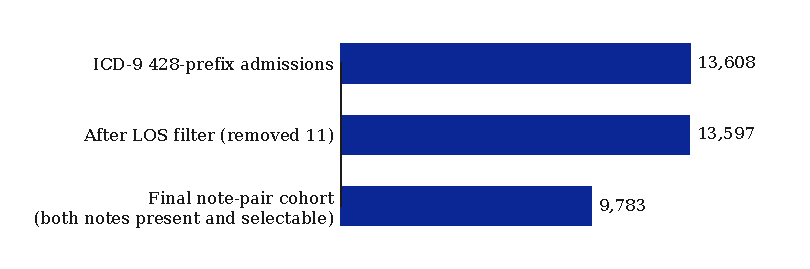
\includegraphics[width=0.92\linewidth]{figures/fig-funnel.pdf}
\caption{Cohort funnel. The reader should notice that the single largest design
decision in the data layer, dropping the third note role, is worth more than a
factor of four in coverage, and that no refinement of the three-role definition
recovered it.}
\label{fig:funnel}
\end{figure}

\begin{figure}[t]
\centering
\framebox[\linewidth]{\parbox[c][5cm][c]{0.92\linewidth}{\centering
\textit{[Figure asset 3.2: two-panel. Left, stacked bar of the 219,683 mentions}
\textit{split classified (88,336) / unclassified (131,347). Right, the 88,336}
\textit{classified mentions split by note role, 79,385 discharge vs 8,951}
\textit{nursing, drawn to scale so the 8.9:1 ratio is visually unavoidable.]}}}
\caption{Extraction yield and the note-role asymmetry. The right panel is the
constraint that governs Chapter~\ref{ch:candidates}: every paired rule is
limited by the smaller population, and every model that consumes a note pair
receives systematically unequal evidence from its two inputs.}
\label{fig:asymmetry}
\end{figure}

\section{Limitations of the Data Layer}
\label{sec:data-limitations}

The following are limitations of this chapter's output, independent of anything
that happens downstream.

\paragraph{Single institution, single era, critical care only.} MIMIC-III covers
one academic medical centre. Documentation conventions, note-type taxonomies,
and medication-list formatting are institution-specific. Nothing in this chapter
transfers without re-derivation.

\paragraph{Billing codes are not clinical phenotypes.} An ICD-9 prefix match
identifies admissions that were \emph{coded} for heart failure. It over-includes
admissions where heart failure is a comorbidity rather than the reason for
admission, and under-includes admissions where it was clinically present but
not coded. The sepsis and AKI cohorts are weaker still.

\paragraph{The extractor is a dictionary, not a clinical NER system.} Recall on
drugs outside the seed list is zero by construction. Negation is a
regular-expression alternation with no scope, and action classification is
window-scoped and first-match. Published clinical medication extraction systems
would be materially better on all three axes \citep{henry2020n2c2}, and the
decision not to use one was driven by an environment problem, not by evidence.

\paragraph{No annotation of the extraction itself.} The extractor's precision
and recall against a human-annotated mention set were never measured. Every
error rate reported later in this thesis is therefore an error rate of the
\emph{composed} system, and the contribution of extraction error to it cannot
be separated from the contribution of candidate-generation error or model error.
This is the most consequential missing measurement in the data layer. A
[TODO: annotate a sample of $n \approx 200$ sentences for drug mention and
action label, and report extractor precision/recall/$F_1$] would resolve it, and
should be the first item of any continuation of this work.

\paragraph{No temporal ordering at sub-day resolution.} Section~\ref{sec:charttime}.

\paragraph{The paired-note design discards within-stay evolution.} One nursing
note per admission, selected as the last one, discards every earlier nursing
note. A medication decision documented at hour 12 and reversed at hour 60 is
invisible; only the hour-60 state enters the pipeline. This is a deliberate
simplification that trades recall of within-stay conflict for tractability, and
it was never revisited.

\section{Ethical Considerations for the Data Layer}
\label{sec:data-ethics}

MIMIC-III is credentialed data governed by a data use agreement. The compliance
posture of this work is stated here in full, including where it is imperfect.

\paragraph{Note text.} No clinical note text appears in this document, in any
figure, table or appendix, or in any released artifact. Files containing
note-derived text are confined to a gitignored local directory outside the
version-controlled tree, and the export script that publishes results scans every
file for note-text markers and aborts rather than filtering on a hit. Released
artifacts are aggregate counts, rates, model scores and pair-level labels.

\paragraph{Third-party services.} The weak labeller in Chapter~\ref{ch:weak} is
an open-weights model run locally; no note text left the analysis machine for
that stage. The GPT-4o comparison reported in Chapter~\ref{ch:eval} was run
against a hosted commercial API, and note excerpts were transmitted to that API
as part of the prompt. Guidance issued during this project's lifetime identifies
transmission of credentialed data to general-purpose hosted APIs as inconsistent
with the data use agreement, and specifies compliant alternatives with
zero-retention and no-human-review terms. The GPT-4o rows are reported with that
caveat attached, and are retained because removing them would misrepresent the
comparison actually performed. No further transmission to hosted services has
occurred and none will occur in follow-on work.

\paragraph{Re-identification and disaggregation.} No re-identification was
attempted and no auxiliary dataset was joined against MIMIC-III at the patient
level. Subgroup analyses are reported as one-way marginals only; no multi-way
disaggregation is published. Cells below approximately ten observations are
reported without suppression, because the source data is de-identified under
HIPAA Safe Harbor and no identifier crosswalk is released. Such cells are
reported for transparency and are not powered to support inference; every claim
resting on them is qualified accordingly in Chapter~\ref{ch:eval}.

\paragraph{Clinical status.} Nothing in this work has been validated for
clinical use. The system is a research artifact evaluated on retrospective
de-identified data, it is not a clinical decision support tool, and its measured
performance --- reported in Chapter~\ref{ch:eval} --- does not support deployment
in any care setting.

\section{Summary}
\label{sec:data-summary}

This chapter produced $19{,}566$ note rows over $9{,}783$ heart-failure
admissions, and $88{,}336$ action-classified medication mentions over $9{,}732$
of them. It also produced four constraints that the rest of the thesis operates
under and cannot escape:

\begin{enumerate}
\item \textbf{The three-role design was abandoned}, at a coverage ceiling of
      $16.8\%$, in favour of a two-role design at $72.2\%$. The cost is that no
      intermediate document exists against which to check whether a conflict was
      resolved before discharge.
\item \textbf{\texttt{CHARTTIME} is null for every discharge summary}, which
      removes sub-day temporal ordering and invalidated a filter that had been
      reported as a clinical finding.
\item \textbf{Action-classified mentions are asymmetric by a factor of $8.9$}
      between discharge summaries and nursing notes, which bottlenecks every
      paired rule and gives every downstream model systematically unequal
      evidence from its two inputs.
\item \textbf{The extractor was never validated}, so no downstream error rate
      can be decomposed into extraction error and model error.
\end{enumerate}

Chapter~\ref{ch:candidates} builds four rules on top of this table and shows
that the mechanism which selects the evidence sentence for each candidate was
wrong for $41.4\%$ of action-conflict candidates.

% ============================================================================
%  Chapter 4. Rule-Based Candidate Generation and the Exemplar Selection Failure
%
%  \input file. Requires booktabs, amsmath, natbib in the parent preamble.
%  Bibliography: accord/thesis/refs.bib
%
%  Traceability: accord/phase3_mining.py (rules, exemplar measurement, splits),
%  accord/dictionaries.py (drug classes, dose parsing), accord/CORRECTIONS.md
%  (C3, C6, C8).
% ============================================================================

\chapter{Rule-Based Candidate Generation and the Exemplar Selection Failure}
\label{ch:candidates}

\section{The Problem This Chapter Solves, and the One It Creates}
\label{sec:cand-overview}

True medication contradictions between a nursing note and a discharge summary
are rare. Chapter~\ref{ch:data} produced $9{,}783$ admissions; a board-certified
pharmacist, annotating a stratified sample drawn from the candidate pool, found
$12$ genuine contradictions in $299$ pairs. Exhaustive human review of all
$9{,}783$ admissions is not feasible, and exhaustive machine scoring of all
cross-note medication pairs is both computationally wasteful and statistically
hostile: the positive class would sit somewhere below one in ten thousand.

Candidate generation is the standard response. A cheap, high-recall,
low-precision rule set narrows the space to a pool that a model or a human can
examine. The rules are not intended to be accurate. They are intended to be
\emph{transparent} and \emph{enriching}: transparent because each candidate
carries a reason, and enriching because the base rate inside the pool should be
far above the base rate outside it.

This chapter constructs four such rules, reports their yield, and then reports
the finding that dominates the chapter and, arguably, the thesis. \emph{The
mechanism that decided which sentence pair to attach to a candidate was
independent of the mechanism that decided the candidate was a conflict.} A
candidate was flagged because the \emph{set} of actions observed for a drug in
one note conflicted with the set observed in the other, but the sentence pair
written into the candidate record was the first mention of that drug on each
side, which need not be, and $41.4\%$ of the time was not, the mention carrying
the conflicting action.

Every consumer of the candidate pool downstream saw only the sentence pair. The
pharmacist annotated the sentence pair. The weak labeller of
Chapter~\ref{ch:weak} read the sentence pair. The model of
Chapter~\ref{ch:arch} was trained on the sentence pair. For a large minority of
candidates, all three were reasoning about evidence that did not contain the
conflict that had caused the candidate to exist.

\section{Problem Formulation}
\label{sec:cand-formulation}

Let an admission $a$ have a nursing note $N_a$ and a discharge summary $D_a$.
Chapter~\ref{ch:data}'s extractor yields, for each note, a set of medication
mentions. Write $M(N_a)$ and $M(D_a)$ for these sets. Each mention
$m$ carries a normalised drug $\mathrm{drug}(m)$, an action label
$\mathrm{act}(m) \in \{\textsc{cess}, \textsc{cont}, \textsc{init},
\textsc{dose}, \textsc{unc}\}$, an optional numeric dose
$(\mathrm{val}(m), \mathrm{unit}(m))$, a sentence $\mathrm{sent}(m)$, and, in
the rebuilt pipeline only, a character offset $\mathrm{pos}(m)$ into the note.

A \emph{candidate} is a tuple
\[
c = \bigl(a,\; r,\; d,\; m_N,\; m_D\bigr),
\]
where $r \in \{1,2,3,4\}$ is the rule that produced it, $d$ is the drug or drug
pair at issue, and $(m_N, m_D)$ is the \emph{exemplar pair}: the single mention
from each note that is presented as evidence.

The distinction that this chapter turns on is between the \emph{trigger
predicate} $T_r(a, d)$, which decides whether a candidate exists, and the
\emph{exemplar selector} $E_r(a, d)$, which decides what $(m_N, m_D)$ is. A
correct implementation requires
\[
T_r \text{ holds} \;\Longrightarrow\; \mathrm{act}(m_N) \text{ and }
\mathrm{act}(m_D) \text{ are the two actions that made } T_r \text{ hold}.
\]
The reference implementation does not satisfy this, because $T_r$ quantifies
over sets of mentions and $E_r$ was implemented as
\texttt{.iloc[0]}, the first row of the drug's mention group.

\section{The Four Rules}
\label{sec:rules}

\subsection{Rule 1: direct action conflict}

Rule 1 fires when the same drug $d$ appears in both notes and the action sets
disagree in a specific direction:
\[
T_1(a,d) \;=\;
\bigl(\textsc{cont} \in A_N \wedge \textsc{cess} \in A_D\bigr)
\;\vee\;
\bigl(\textsc{cess} \in A_N \wedge \textsc{cont} \in A_D\bigr),
\]
where $A_N = \{\mathrm{act}(m) : m \in M(N_a), \mathrm{drug}(m) = d\}$ and $A_D$
is defined analogously. This is the canonical case: the nursing note records the
drug as held and the discharge summary orders it continued, or the reverse.

Note the existential quantifier. Rule 1 fires if \emph{some} mention on each
side carries the required action. A drug mentioned five times in a discharge
summary with four continuation mentions and one cessation mention satisfies the
predicate. This is deliberate and correct for a high-recall trigger. It is also
precisely what makes the exemplar selection problem non-trivial.

\subsection{Rule 2: drug class conflict}

Rule 2 generalises Rule 1 to the pharmacologic class. Two \emph{different} drugs
in the same class, one continued and one ceased across the two notes, may
represent a substitution that was documented on one side and not the other. It
uses a hand-written dictionary of $10$ classes covering $31$ drugs
(ACE inhibitors, ARBs, beta blockers, loop diuretics, anticoagulants, statins,
insulins, nitrates, antiarrhythmics, aldosterone antagonists). The predicate is
$T_1$ with the drug identity relaxed to class identity, plus a guard that the
drug sets on the two sides are not identical, which would return the candidate
to Rule 1's territory.

The class dictionary is a limitation in itself. Ten classes and $34$ drugs is a
small fraction of the pharmacologic space, it is not derived from a standard
terminology such as ATC or RxNorm, and its class boundaries encode one author's
judgement. It has no mechanism for cross-class interactions, which are a large
share of clinically significant medication problems.

\subsection{Rule 3: dosage conflict}

Rule 3 fires when the same drug carries a parseable numeric dose in both notes,
the two doses reduce to the same canonical unit, and they differ by more than
$20\%$ of the larger value:
\[
T_3(a,d) \;=\; \exists\, (m_N, m_D) :\;
\mathrm{unit}(m_N) = \mathrm{unit}(m_D)
\;\wedge\;
\frac{\max - \min}{\max} > 0.20 .
\]
The $20\%$ threshold is a judgement call with no empirical derivation. It is not
tuned, and it is not clinically grounded in the sense that different drug
classes tolerate very different dose variation. A $25\%$ change in a statin dose
and a $25\%$ change in a warfarin dose are not comparable events. This is a
known weakness of the rule and it is not addressed anywhere in this thesis.

Rule 3's exemplar selection is correct by construction: the exemplar pair is the
$(m_N, m_D)$ pair achieving the largest percentage difference, so it necessarily
carries the conflict. There is no \texttt{.iloc[0]} defect to fix here, because
the rule had no reference implementation at all. It exists only in the rebuild,
for the reason given in Chapter~\ref{ch:data}: the reference extractor stored
dose strings and never parsed them to numbers, so there was nothing to compute a
percentage from.

\subsection{Rule 4: omission conflict}

Rule 4 fires when a drug receives a cessation action in the nursing note and is
\emph{absent} from every extracted mention in the discharge summary, classified
or not:
\[
T_4(a,d) \;=\;
\bigl(\exists\, m \in M(N_a) : \mathrm{drug}(m) = d \wedge
\mathrm{act}(m) = \textsc{cess}\bigr)
\;\wedge\;
d \notin \{\mathrm{drug}(m) : m \in M(D_a)\}.
\]
This is the clinically most interesting rule and the one with the weakest
evidence, because absence is not the same as a decision. A drug held at the
bedside and never mentioned again in the discharge summary may have been
deliberately discontinued and correctly omitted, or may have been dropped from
the discharge list by oversight. The rule cannot distinguish these, and neither
can the sentence pair it produces, because there is no discharge sentence: the
discharge side of a Rule 4 candidate is the literal string \texttt{absent}.

That property is worth flagging now and is returned to in
Chapter~\ref{ch:weak}: Rule 4 is the only rule whose candidates present the
downstream consumer with a structurally different input, a nursing sentence
paired with an empty string. It is also the only rule on which the weak
labeller and the trained model behave differently from the other three.

\section{Candidate Yield}
\label{sec:cand-yield}

\begin{table}[t]
\centering
\small
\begin{tabular}{clrr}
\toprule
\textbf{Rule} & \textbf{Trigger} & \textbf{Candidates} & \textbf{Admissions} \\
\midrule
1 & Direct action conflict (same drug, opposite actions) & 886   & 701 \\
2 & Drug class conflict (same class, different agents)   & 203   & 195 \\
3 & Dosage conflict ($>20\%$ difference)                 & 521   & n/a \\
4 & Omission (held in nursing, absent from discharge)    & 370   & n/a \\
\midrule
  & \textbf{Total raw}                                   & \textbf{1,980} & n/a \\
  & \textbf{After temporal prefilter}                    & \textbf{1,978} & \textbf{1,203} \\
\bottomrule
\end{tabular}
\caption{Candidate yield by rule. Per-rule admission counts were preserved in
the run log only for Rules 1 and 2. The temporal prefilter removed two
candidates in total; Chapter~\ref{ch:data}, Section~\ref{sec:charttime},
explains why this filter should be understood as an instrument failure rather
than a measurement, and why the two-candidate reduction carries no information.}
\label{tab:yield-rules}
\end{table}

Table~\ref{tab:yield-rules} reports the pool. Two observations.

First, the pool is small relative to the cohort: $1{,}978$ candidates from
$9{,}783$ admissions, so roughly one admission in eight contributes a candidate,
and the $1{,}978$ candidates come from only $1{,}203$ distinct admissions, about
$1.64$ candidates per contributing admission. The concentration is not
incidental; Section~\ref{sec:splits} shows that it is the reason a row-level
train/test split leaks.

Second, the drug distribution is dominated by a handful of agents, shown in
Table~\ref{tab:top-drugs}. Furosemide alone accounts for $373$ candidates,
nearly a fifth of the pool.

\begin{table}[t]
\centering
\small
\begin{tabular}{lrl}
\toprule
\textbf{Drug} & \textbf{Candidates} & \textbf{Class} \\
\midrule
Furosemide  & 373 & Loop diuretic \\
Metoprolol  & 297 & Beta blocker \\
Heparin     & 166 & Anticoagulant \\
Warfarin    & 145 & Anticoagulant \\
Amiodarone  & 110 & Antiarrhythmic \\
\bottomrule
\end{tabular}
\caption{The five most frequent drugs in the candidate pool. These five account
for $1{,}091$ of $1{,}978$ candidates. Within Rule 2, anticoagulants contribute
$107$ of $203$ candidates and beta blockers $34$, so two of ten classes supply
$69\%$ of the class-conflict pool. A model trained on this pool sees a small
number of drugs repeatedly and has ample opportunity to key on drug identity
rather than on the relationship between the two sentences.}
\label{tab:top-drugs}
\end{table}

\section{The Exemplar Selection Failure}
\label{sec:exemplar}

\subsection{The defect}

The reference mining code for Rules 1 and 2 has the following shape:

\begin{quote}\ttfamily\small
conflict = ('continuation' in n\_actions and 'cessation' in d\_actions) \\
\hphantom{conflict = }or ('cessation' in n\_actions and 'continuation' in d\_actions) \\
if conflict: \\
\hphantom{if }n\_row = nursing[nursing['drug'] == drug].iloc[0] \\
\hphantom{if }d\_row = discharge[discharge['drug'] == drug].iloc[0]
\end{quote}

The first two lines evaluate the trigger over sets. The last two lines select
the exemplar by positional index into the drug's mention group. Nothing
constrains \texttt{n\_row} and \texttt{d\_row} to carry the actions that made
\texttt{conflict} true.

The failure mode is concrete. Suppose a discharge summary mentions furosemide
five times: four windows resolve to \emph{continuation} and one, later in the
note, resolves to \emph{cessation}. Suppose the nursing note has a single
\emph{continuation} mention. Then $A_N = \{\textsc{cont}\}$,
$A_D = \{\textsc{cont}, \textsc{cess}\}$, the trigger fires on the
$(\textsc{cont}, \textsc{cess})$ branch, and the candidate is real by the rule's
own definition. But \texttt{.iloc[0]} on the discharge side returns a
\emph{continuation} row. The exemplar pair that the pipeline labels a
contradiction consists of two sentences in which the two notes \emph{agree}.

\subsection{Why the defect was invisible}

Chapter~\ref{ch:data} noted that the reference mentions table stored no
positional information. That is the enabling condition. Without a sentence index
or a character offset, mentions of the same drug within the same note are
indistinguishable rows, and \texttt{.iloc[0]} is not obviously different from any
other choice; there was no representation in which ``the mention that carries
the conflict'' could be expressed. The bug is therefore not a typo. It is a
consequence of an upstream schema decision, and it is the clearest instance in
this project of the pattern that \citet{sculley2015debt} describe as
configuration and data-dependency debt: a defect made unreachable by the absence
of the field that would have exposed it.

\subsection{The fix}

The rebuilt implementation (\texttt{accord/phase3\_mining.py}) selects, on each
side independently, among only those mentions whose \emph{own} action equals the
action required by that specific candidate's conflict branch:
\[
E_r^{\text{new}}(a,d) = \bigl(\arg\!\min_{m \in C_N} \delta(m),\;
\arg\!\min_{m \in C_D} \delta(m)\bigr),
\]
\[
C_N = \{m : \mathrm{drug}(m)=d,\ \mathrm{act}(m) = \rho_N\}, \quad
C_D = \{m : \mathrm{drug}(m)=d,\ \mathrm{act}(m) = \rho_D\},
\]
where $(\rho_N, \rho_D)$ is the required action pair for the branch that fired,
and $\delta(m)$ is the character distance from $m$ to the nearest dose-bearing
mention in the same note. The tie-break is a heuristic with a stated rationale:
a mention adjacent to a concrete dose is more likely to be a substantive
instruction than a passing reference in an allergy list or a problem list. If no
dose-bearing mention exists in the note, the tie-break falls back to the
earliest qualifying sentence, for determinism.

The tie-break is not validated. It affects only which of several
\emph{qualifying} mentions is chosen, so it cannot reintroduce the original
defect, but the claim that dose adjacency indicates clinical substance is an
assumption. [TODO: measure whether the dose-adjacency tie-break changes the
pharmacist's judgement relative to an earliest-sentence tie-break, on a sample
of candidates where the two disagree.]

\subsection{The measurement}

The rebuild instruments both selectors and records, for every action-conflict
candidate, whether the old exemplar's action pair matched the required pair and
whether the fix changed the selected rows. Table~\ref{tab:exemplar} reports the
result.

\begin{table}[t]
\centering
\small
\begin{tabular}{lrr}
\toprule
 & \textbf{Old exemplar correct} & \textbf{Exemplar changed by fix} \\
\midrule
Rule 1 (direct action conflict) & 60.5\% & n/a \\
Rule 2 (drug class conflict)    & 50.4\% & n/a \\
\midrule
\textbf{Rules 1 $+$ 2 pooled}   & \textbf{58.6\%} & \textbf{739 / 1,307 (56.5\%)} \\
\bottomrule
\end{tabular}
\caption{Exemplar correctness under the reference selector. ``Old exemplar
correct'' is the fraction of action-conflict candidates for which the
\texttt{.iloc[0]} exemplar pair actually carried the two actions that triggered
the candidate. The complement, $41.4\%$, is the fraction of action-conflict
candidates justified to every downstream consumer by a sentence pair that did
not contain the conflict. Rule 2 is worse than Rule 1, as expected: class-level
conflicts quantify over more mentions, so the probability that the first mention
happens to be the conflicting one is lower. The rebuild mined $1{,}307$
action-conflict candidates against the reference's $1{,}089$
($886 + 203$), because it runs against the corrected cohort of
Chapter~\ref{ch:data} and an offset-bearing mentions table; the rate is measured
on the rebuild's pool and is reported as such.}
\label{tab:exemplar}
\end{table}

Three readings of Table~\ref{tab:exemplar} are worth separating.

\paragraph{As a bug report.} $41.4\%$ of action-conflict candidates carried
evidence inconsistent with their own trigger, and $56.5\%$ of them change
exemplar under the fix. The two numbers differ because a candidate can change
exemplar on one side while the old exemplar happened to be correct on the other,
or vice versa.

\paragraph{As a bound on annotation validity.} The pharmacist annotated the
exemplar pair. For roughly two in five action-conflict candidates, the sentence
pair presented did not contain the flagged conflict. The pharmacist's judgement
on those pairs is a correct judgement about the wrong evidence. This means the
$4.0\%$ contradiction rate reported in Section~\ref{sec:gold} is an
\textbf{upper bound on the validity of the annotation exercise}, not a clean
estimate of the candidate pool's precision. Whether the true precision is higher
or lower is not determinable from the data collected, because we do not know how
the pharmacist would have ruled on the corrected exemplars. This limitation is
restated in every chapter that uses the $4.0\%$ figure.

\paragraph{As a scoping constraint.} The exemplar defect contaminates
\emph{annotation}. It does not contaminate the measurements in
Chapter~\ref{ch:eval} that are computed on model scores against the annotation:
the AUROC, the threshold sweep, the severity correlations, and the transfer
collapse are all statements about whether the model's output ordering carries
information about the pharmacist's label, whatever that label was measured
against. If the model had learned anything from the exemplar sentences, it would
show up as ranking signal against those same sentences. It does not.
Section~\ref{sec:eval-scoping} in Chapter~\ref{ch:eval} makes this argument
formally.

\section{The Gold Standard}
\label{sec:gold}

\subsection{Sampling}

A stratified sample of $300$ candidates was drawn from the $1{,}978$-pair pool,
allocated across rules as shown in Table~\ref{tab:gold}. The allocation
oversamples Rules 2 and 4 relative to their share of the pool, on the reasoning
that these are the rules whose behaviour was least understood.

\subsection{Annotation protocol}

A single board-certified pharmacist annotated $299$ of the $300$ sampled
pairs.\footnote{The sampling frame is $300$; $299$ annotations were returned.
[TODO: identify which stratum lost a row. The per-rule rates in
Table~\ref{tab:gold} are computed against the $300$-row stratum sizes, which
reproduce the reported percentages exactly, so the missing row's stratum cannot
be recovered from the rates alone.]} For each pair the annotator recorded a
three-way label (\emph{contradiction}, \emph{not a contradiction},
\emph{ambiguous}), a free-text justification, a confidence rating, and, for
contradictions, a $1$ to $5$ danger rating.

Annotation was performed in two passes separated by a two-week washout. This
controls for within-session drift and fatigue. It does not establish inter-rater
reliability, because there is one rater.

\subsection{A retracted reliability claim}

The project previously reported a Cohen's $\kappa$ of $1.000$ between ``two
independent pharmacist judgement instruments,'' offered as an answer to reviewer
requests for inter-rater reliability. That claim is withdrawn. The two
``instruments'' were the binary contradiction label and the $1$ to $5$ danger
rating. A pair that is not a contradiction has no danger by definition, so
$\texttt{label} = \textit{contradiction} \iff \texttt{danger} > 0$ is an
identity and $\kappa = 1.000$ is guaranteed by construction
\citep{cohen1960kappa}. It measures nothing about annotator reliability.

The honest statement is the one made here: this study has one annotator, a
two-pass protocol with a two-week washout, and \textbf{no established inter-rater
reliability}. With $12$ positives in $299$ pairs, a second annotator would be
the highest-value single addition to this work, and the absence of one is a
first-order limitation on every conclusion that rests on the gold labels.

\subsection{Results}

\begin{table}[t]
\centering
\small
\begin{tabular}{clrrrr}
\toprule
\textbf{Rule} & \textbf{Trigger} & \textbf{Sampled} & \textbf{True} & \textbf{Rule} & \textbf{ACCORD} \\
              &                  &                  & \textbf{contra.} & \textbf{precision} & \textbf{precision} \\
\midrule
1 & Direct action conflict & 134 & 3 & 2.2\% & 2.3\% \\
2 & Drug class conflict    & 31  & 3 & 9.7\% & 10.0\% \\
3 & Dosage conflict        & 79  & 4 & 5.1\% & 5.2\% \\
4 & Omission               & 56  & 2 & 3.6\% & 2.4\% \\
\midrule
  & \textbf{Pooled}        & \textbf{300} & \textbf{12} & \textbf{4.0\%} & \textbf{4.7\%} \\
\bottomrule
\end{tabular}
\caption{Gold-standard results by rule. ``Rule precision'' is the fraction of
that rule's annotated candidates the pharmacist judged to be true
contradictions, that is, the rule's own precision as a detector. ``ACCORD
precision'' is the precision of the trained detector of Chapter~\ref{ch:arch}
restricted to that rule's candidates, reported here for direct comparison and
derived in full in Chapter~\ref{ch:eval}. The per-rule true-contradiction counts
$(3,3,4,2)$ are derived from the reported rates and stratum sizes and sum to the
$12$ observed positives. Sampled counts are the stratum sizes of the $300$-row
frame; $299$ annotations were returned.}
\label{tab:gold}
\end{table}

Of $299$ annotated pairs: $12$ contradictions ($4.0\%$), $241$ not
contradictions, and $46$ ambiguous ($15.4\%$). The ambiguous rate is itself a
result. One in six candidates could not be adjudicated by a board-certified
pharmacist from the presented evidence. Some of that is the exemplar defect,
some is the inherent underspecification of a two-sentence view of a medication
decision, and the two cannot be separated with the data collected.

\subsection{The finding in Table~\ref{tab:gold}}

Read the last two columns together. For Rules 1, 2, and 3, ACCORD's precision on
a rule's candidates is essentially identical to that rule's own base rate:
$2.3$ against $2.2$, $10.0$ against $9.7$, $5.2$ against $5.1$. For Rule 4 it is
\emph{below} the base rate, $2.4$ against $3.6$.

The interpretation is direct. A detector that adds discriminative value on top
of a rule should have precision above that rule's base rate, because it should
be discarding some of the rule's false positives. ACCORD does not. Its precision
tracks the base rate because it predicts \emph{positive} for essentially every
candidate the rules hand it, in which case precision is arithmetically forced to
approximately the base rate divided by the predicted-positive rate.
Chapter~\ref{ch:weak} shows where that near-universal positive prediction comes
from, and Chapter~\ref{ch:eval} shows that it holds at every threshold, not just
at $0.5$.

The Rule 4 case is the informative exception. Rule 4 is the only rule on which
the model does \emph{not} predict positive almost universally (it predicts
positive at $74.5\%$), and it is the only rule on which the model's precision
falls below the base rate. Arithmetically, ACCORD recovers only one of the two
true Rule 4 contradictions, which accounts for both the precision drop and the
single miss in the $11/12$ recall reported in Chapter~\ref{ch:eval}. Where the
model exercises any selectivity at all, it selects wrongly.

\section{Splitting, and Why the Reference Split Leaked}
\label{sec:splits}

The reference pipeline split the candidate pool at the row level:

\begin{quote}\ttfamily\small
labels\_df = labels[labels['weak\_label'] != 'ambiguous'].sample(frac=1, random\_state=42) \\
train\_df = labels\_df.iloc[:int(n*0.8)]
\end{quote}

With $1{,}978$ candidates drawn from $1{,}203$ admissions, and with a patient
population that has known repeat admissions, this places candidates that share a
nursing note, a discharge summary, an admission, or a patient on both sides of
the split. Two candidates from the same admission differ only in the drug at
issue; the surrounding note text, the de-identification surrogates, and the
documentation style are identical. A model that memorises note-level surface
features will score them together.

The rebuild splits by \texttt{SUBJECT\_ID} with disjointness asserted in code:
\[
S_{\text{train}} \cap S_{\text{val}} = S_{\text{train}} \cap S_{\text{test}}
= S_{\text{val}} \cap S_{\text{test}} = \emptyset,
\qquad
S_{\text{train}} \cup S_{\text{val}} \cup S_{\text{test}} = S .
\]
Patient-level grouping is the correct unit here because it is the only unit that
guarantees no shared note and no shared documentation episode. Assertions rather
than comments are used deliberately: the reference pipeline's split was not
wrong because the author believed row-level splitting was acceptable, it was
wrong because nothing in the code would have complained.

All results reported in Chapters~\ref{ch:arch} and~\ref{ch:eval} for the trained
model use a held-out set that excludes the $299$ annotated pairs. An earlier
reported configuration trained on the full $1{,}978$-pair pool, which contains
those $299$ pairs. That configuration is training on the evaluation set, its
results are not reported anywhere in this thesis, and the reader should treat
any earlier project artifact quoting it as superseded.

\section{Proposed Figures}
\label{sec:cand-figures}

\begin{figure}[t]
\centering
\framebox[\linewidth]{\parbox[c][6cm][c]{0.92\linewidth}{\centering
\textit{[Figure asset 4.1: schematic of the exemplar defect. Two columns,}
\textit{``nursing note'' and ``discharge summary''. Each column shows five}
\textit{abstract mention slots with action tags (no clinical text). The}
\textit{discharge column has four CONT slots and one CESS slot at position 5.}
\textit{An arrow labelled ``trigger: sets conflict'' spans both columns. A}
\textit{second arrow labelled \texttt{.iloc[0]} points at slot 1 (CONT). A}
\textit{third arrow labelled ``fix: action-matched + dose-adjacent'' points at}
\textit{slot 5 (CESS). Caption box: ``the pair shown to the annotator, the LLM,}
\textit{and the model is the \texttt{.iloc[0]} pair''.]}}}
\caption{The exemplar selection defect. The trigger predicate quantifies over
sets of mentions; the exemplar selector indexes positionally. Nothing forces the
two to agree, and for $41.4\%$ of action-conflict candidates they did not. No
clinical text appears in this figure; slots are abstract.}
\label{fig:exemplar}
\end{figure}

\begin{figure}[t]
\centering
\framebox[\linewidth]{\parbox[c][5cm][c]{0.92\linewidth}{\centering
\textit{[Figure asset 4.2: grouped bar chart, one group per rule. Bars: (a)}
\textit{rule precision from the pharmacist, 2.2 / 9.7 / 5.1 / 3.6; (b) ACCORD}
\textit{precision on that rule's candidates, 2.3 / 10.0 / 5.2 / 2.4. A dashed}
\textit{horizontal line at the pooled 4.0\% base rate. Rule 4's pair is the only}
\textit{one where (b) is below (a); highlight it.]}}}
\caption{ACCORD's precision tracks each rule's own base rate. The reader should
notice that the model contributes no lift over the rule that generated the
candidate on any of the four rules, and that on Rule 4, the only rule where it
declines a substantial fraction of candidates, its precision falls below the
base rate.}
\label{fig:rule-precision}
\end{figure}

\section{Limitations}
\label{sec:cand-limitations}

\paragraph{The rules encode one author's clinical judgement.} The class
dictionary, the $20\%$ dose threshold, the choice of four rules rather than
forty, and the decision to treat absence as evidence in Rule 4 are all
unvalidated design choices. No clinician reviewed the rule set before it was
run.

\paragraph{Rules 3 and 4 have no reference implementation.} They exist only in
the rebuild. Any comparison between rebuild and reference behaviour is therefore
restricted to Rules 1 and 2, which is why Table~\ref{tab:exemplar} covers only
those two.

\paragraph{The exemplar defect bounds annotation validity, and the bound is
one-sided in an unknown direction.} We know $41.4\%$ of action-conflict
candidates were annotated against evidence that did not carry their conflict. We
do not know how the pharmacist would have ruled on corrected evidence. Both a
higher and a lower true precision are consistent with the data. Re-annotating a
sample of the changed candidates under the corrected selector is the single
measurement that would resolve this, and it was not performed. [TODO: re-annotate
$n \approx 100$ of the $739$ changed candidates and report the label-change
rate.]

\paragraph{One annotator.} Section~\ref{sec:gold}. Twelve positives is a small
number on which to rest a benchmark, and the confidence intervals in
Chapter~\ref{ch:eval} reflect that.

\paragraph{The candidate pool bounds recall absolutely.} Nothing outside the
$1{,}978$ candidates can ever be detected by this pipeline. The rules' recall
against the full set of true contradictions in the $9{,}783$ admissions is
unmeasured and unmeasurable without exhaustive review. Every recall figure in
this thesis is recall \emph{within} the candidate pool.

\section{Summary}
\label{sec:cand-summary}

Four rules produce $1{,}978$ candidates over $1{,}203$ admissions, enriched to a
pharmacist-measured base rate of $4.0\%$ from a background rate that is orders
of magnitude lower. That much works.

The chapter's principal finding is that the enrichment came with a defect that
was invisible to every downstream consumer. For $41.4\%$ of action-conflict
candidates, the sentence pair carrying the justification did not carry the
conflict, because the trigger quantified over sets while the exemplar selector
indexed positionally, and because the upstream schema had no field in which the
distinction could be expressed. The fix changes the exemplar for $739$ of
$1{,}307$ candidates.

The consequence is a bound, not a correction: the $4.0\%$ figure is an upper
bound on the validity of the annotation exercise rather than an estimate of the
pipeline's precision. Chapter~\ref{ch:eval} shows that this bound does not
compromise the negative result, because the negative result is measured on
model scores against the same annotations, and the model's scores turn out to
carry no information about those annotations at all.

Chapter~\ref{ch:weak} takes the candidate pool and asks a language model to
label it.

% ============================================================================
%  Chapter 5. Weak Supervision and the Inherited Prior
%
%  \input file. Requires booktabs, amsmath, natbib in the parent preamble.
%  Bibliography: accord/thesis/refs.bib
%
%  Traceability: accord/CORRECTIONS.md (C9), the weak-labelling run logs, and
%  the per-rule predicted-positive rates recorded in the audit outputs.
% ============================================================================

\chapter{Weak Supervision and the Inherited Prior}
\label{ch:weak}

\section{The Question This Chapter Answers}
\label{sec:weak-overview}

Chapter~\ref{ch:candidates} produced $1{,}978$ candidate pairs and, for $299$ of
them, a pharmacist's judgement. Training a supervised detector on $299$
annotations containing $12$ positives is not viable. The standard remedy is weak
supervision: obtain approximate labels cheaply for the remaining pool, accept
that they are noisy, and rely on the model to average over the noise
\citep{ratner2017snorkel}. Since 2023 the dominant cheap labeller has been an
instruction-tuned language model, on the strength of results showing that such
models match or exceed crowd annotators on several classification tasks
\citep{gilardi2023chatgpt}.

This chapter reports what happened when that recipe was applied to
cross-note medication contradiction detection, and it is the clearest example in
this thesis of a failure that is entirely diagnosable in advance and was not
diagnosed.

\paragraph{Research question.} Can an instruction-tuned open-weights language
model supply usable weak labels for a rare, clinically technical, pairwise
judgement, in a regime where the true positive rate is around $4\%$?

\paragraph{Answer.} No, and the failure is not one of accuracy on individual
examples. It is a failure of \emph{prior}. The labeller assigned the positive
class to $84.9\%$ of candidates against a pharmacist-measured base rate of
$4.0\%$, a prevalence mismatch of roughly $21\times$. The detector trained on
those labels reproduced the labeller's per-rule positive rate almost exactly,
which is the behaviour of a student that has learned its teacher's marginal and
nothing about the input.

\section{Setup}
\label{sec:weak-setup}

\subsection{Labeller and pool}

The weak labeller is Llama 3 8B \citep{grattafiori2024llama3}, run locally. It
was presented with each candidate's exemplar pair, the nursing sentence and the
discharge sentence, together with the rule that generated the candidate, and
asked for a binary judgement: \emph{contradiction} or \emph{not\_contradiction},
plus a confidence value.

The labelled pool is $1{,}679$ rows. This is exactly the $1{,}978$ candidates of
Chapter~\ref{ch:candidates} minus the $299$ pairs sent to the pharmacist, so the
weak-label training set and the gold evaluation set are disjoint by
construction. That part of the design is correct and is worth stating, because
much else in this chapter is not.

\subsection{What the labeller was shown}

The labeller saw the exemplar sentence pair. Chapter~\ref{ch:candidates},
Section~\ref{sec:exemplar}, established that for $41.4\%$ of action-conflict
candidates the exemplar pair did not carry the conflict that triggered the
candidate, while the prompt asserted, via the rule identifier, that a conflict
of that type was present. The labeller was therefore told, for a large minority
of rows, that a conflict existed in a sentence pair that did not exhibit one.
Section~\ref{sec:weak-acquiescence} argues that this is one of several mutually
reinforcing pressures towards the positive class, and that the design contained
no mechanism for any of them to be detected.

\section{The Prevalence Mismatch}
\label{sec:weak-prevalence}

\begin{table}[t]
\centering
\small
\begin{tabular}{lrr}
\toprule
 & \textbf{Count} & \textbf{Rate} \\
\midrule
Weak label $=$ \emph{contradiction}      & 1,425 & 84.9\% \\
Weak label $=$ \emph{not\_contradiction} & 254   & 15.1\% \\
\midrule
Total labelled                            & 1,679 & \\
\midrule
Pharmacist base rate (gold, $n{=}299$)    & 12 & 4.0\% \\
\midrule
\textbf{Prevalence ratio}                 & & \textbf{$\approx 21\times$} \\
\bottomrule
\end{tabular}
\caption{The weak labeller's marginal against the measured base rate. The
labeller assigns the positive class at roughly twenty-one times the rate a
board-certified pharmacist does. This is the single number that determines
everything the trained model subsequently does.}
\label{tab:prevalence}
\end{table}

Table~\ref{tab:prevalence} is the chapter's central result. Two derivations make
its severity concrete. Both are arithmetic from the reported counts and are
labelled as derived.

\paragraph{Derivation 1: the floor on false positives.} If the pharmacist's
$4.0\%$ base rate holds in the unlabelled pool, then approximately $67$ of the
$1{,}679$ rows are true contradictions. The labeller calls $1{,}425$ of them
positive. Even granting the labeller perfect recall, at least
$1{,}425 - 67 = 1{,}358$ of its positive labels are wrong. More than $95\%$ of
the positive supervision signal is noise, and it is not symmetric noise: it is
concentrated entirely in one class.

\paragraph{Derivation 2: the label is nearly constant.} A label that takes one
value $84.9\%$ of the time carries little information about the input regardless
of how it is distributed. Under this supervision, the loss-minimising strategy
for a model with sufficient capacity to fit the marginal but insufficient signal
to fit the conditional is to predict the majority class with high confidence.
Section~\ref{sec:weak-tracking} shows that this is what happened.

\paragraph{Why standard weak-supervision theory does not rescue this.}
Aggregation frameworks such as Snorkel \citep{ratner2017snorkel} are designed for
noise that is \emph{conditionally independent across sources given the true
label}, and their guarantees rest on having multiple sources whose errors are
not aligned. Here there is one source. Its error is a systematic prior shift, not
independent noise, and no amount of downstream averaging removes a shifted
marginal. The recipe was applied outside the regime in which it works.

\section{The Student Inherits the Teacher's Marginal}
\label{sec:weak-tracking}

\begin{table}[t]
\centering
\small
\begin{tabular}{clrrr}
\toprule
\textbf{Rule} & \textbf{Trigger} & \textbf{Llama} & \textbf{ACCORD} & \textbf{True} \\
              &                  & \textbf{pos.\ rate} & \textbf{pos.\ rate} & \textbf{prevalence} \\
\midrule
1 & Direct action conflict & 95.5\% & 97.0\% & 2.2\% \\
2 & Drug class conflict    & 96.8\% & 96.8\% & 9.7\% \\
3 & Dosage conflict        & 98.7\% & 97.5\% & 5.1\% \\
4 & Omission               & 45.5\% & 74.5\% & 3.6\% \\
\bottomrule
\end{tabular}
\caption{Predicted-positive rates by rule. ``Llama pos.\ rate'' is the fraction
of that rule's candidates the weak labeller called a contradiction; ``ACCORD
pos.\ rate'' is the fraction the trained detector predicts positive at threshold
$0.5$; ``true prevalence'' is the pharmacist-measured rate from
Table~\ref{tab:gold}. On Rules 1 to 3 the student tracks the teacher to within
$1.5$ percentage points while both sit an order of magnitude above the truth.
Rule 4 is the exception, and the direction of the exception is diagnostic:
ACCORD does not reproduce the teacher's selectivity, it regresses towards its
own global positive prior.}
\label{tab:tracking}
\end{table}

Table~\ref{tab:tracking} is the mechanism behind Chapter~\ref{ch:eval}'s
results. Three readings.

\paragraph{Rules 1 to 3: near-perfect marginal transfer.} The student's positive
rate differs from the teacher's by $1.5$, $0.0$, and $1.2$ percentage points.
Meanwhile the true prevalence varies by more than a factor of four across those
same three rules ($2.2\%$, $9.7\%$, $5.1\%$). The student reproduces the
quantity that carries no information about the truth and does not reproduce the
quantity that does. This is not a model that learned a noisy version of the
task. It is a model that learned the label's marginal distribution.

\paragraph{Rule 4: the teacher's one real distinction, discarded.} The weak
labeller behaves visibly differently on Rule 4, calling only $45.5\%$ of
omission candidates positive against $95\%$ to $99\%$ elsewhere. There is a plain
explanation: Rule 4 candidates have an \emph{empty} discharge side, since the
drug is absent from the discharge summary by construction. Presented with a
sentence and nothing to compare it to, the labeller declines roughly half the
time. Whether this reflects clinical reasoning or a formatting response to a
degenerate input cannot be determined from the labels alone, and the distinction
matters: the true prevalence on Rule 4 is $3.6\%$, so even at $45.5\%$ the
labeller is still more than twelve times too positive.

What the student does with this is the informative part. ACCORD's Rule 4
positive rate is $74.5\%$, roughly midway between the teacher's $45.5\%$ and its
own global rate. The one place where the supervision carried a real
input-dependent signal is the one place where the student partially discarded
it, pulling towards its majority prior. A model learning the conditional would
have sharpened the distinction; a model learning the marginal blunts it.

\paragraph{The consequence for precision.} If a detector predicts positive at
rate $p$ on a subpopulation whose true prevalence is $\pi$, and its predictions
are independent of the label, its precision is $\pi / p \cdot p = \pi$ in
expectation, that is, exactly the base rate. Table~\ref{tab:gold} in
Chapter~\ref{ch:candidates} shows precisely this: $2.3$ against $2.2$, $10.0$
against $9.7$, $5.2$ against $5.1$. The apparent variation in ACCORD's precision
across rules is entirely explained by variation in the rules' own base rates.

\section{The Degenerate Confidence Field}
\label{sec:weak-confidence}

\subsection{The finding}

The weak labelling produced a \texttt{weak\_confidence} field alongside each
label. Across all $1{,}679$ training rows and all $299$ audit rows it takes
exactly two values:
\[
\texttt{weak\_confidence} =
\begin{cases}
0.95 & \text{iff } \texttt{weak\_label} = \textit{contradiction},\\
1.00 & \text{iff } \texttt{weak\_label} = \textit{not\_contradiction}.
\end{cases}
\]
It is a deterministic function of the label. It contains no information about
the labeller's uncertainty on any individual example, and it cannot, because it
does not vary within a label class.

\subsection{Why this is worse than a useless field}

An unused useless field is harmless. This one was used, in two places, both of
which convert a label into a training-time intervention.

\paragraph{As a filter.} The training code discards rows with
$\texttt{weak\_confidence} < 0.9$. Since the field's minimum value is $0.95$,
this filter removes nothing. It is a no-op that reads, in the code and in every
description of the pipeline, as a quality-control step. Its presence created the
appearance of confidence-based data cleaning where none occurred.

\paragraph{As a loss weight.} The same field is multiplied into the per-example
loss. Because the field is a function of the label, this is a
\emph{label-conditioned reweighting}: every positive example's loss is scaled by
$0.95$ and every negative's by $1.00$. The direction is perverse. The positive
class is already the overwhelming majority at $84.9\%$, and the reweighting
further downweights it by $5\%$ relative to the minority class, which is a
five-percent nudge in the right direction applied to a twenty-one-fold error in
the wrong one. The magnitude is negligible; the fact that the pipeline contained
a label-dependent loss weight that nobody intended is not.

\subsection{The general lesson}

A confidence field emitted by a language model alongside a label is not a
calibrated probability and should not be treated as one without measurement
\citep{guo2017calibration,zhao2021calibrate}. The specific diagnostic that
would have caught this is trivial and should be mandatory: \emph{print the
number of distinct values a confidence field takes, and its conditional
distribution given the label, before using it for anything}. Two distinct
values, perfectly separated by label, is a result that takes one line of code to
obtain and ends the discussion.

\section{Why the Labeller Says Yes}
\label{sec:weak-acquiescence}

The chapter has established that the labeller is systematically positive. It is
worth separating the candidate explanations, because they have different
remedies and because this thesis is not in a position to adjudicate between
them.

\paragraph{The prompt asserts the conclusion.} Each candidate was presented
together with the rule that produced it, which names a conflict type. A prompt
that says ``this pair was flagged as a direct action conflict; is it a
contradiction?'' contains its own answer. This is the most likely dominant
cause and the cheapest to test.

\paragraph{The evidence frequently does not support the assertion.} For $41.4\%$
of action-conflict candidates the exemplar pair did not carry the conflict
(Chapter~\ref{ch:candidates}). A labeller that resolves the tension between a
confident framing and unsupportive evidence in favour of the framing will be
systematically positive, and will be so most often exactly where the evidence is
weakest.

\paragraph{Class-prior insensitivity.} Instruction-tuned models are known to
carry strong, prompt-sensitive class priors that do not track the true base rate
of the task \citep{zhao2021calibrate}. A task with a $4\%$ positive rate is far
outside the regime where an unanchored prior is harmless.

\paragraph{Failure defaults.} A related component of this project scored every
unparseable generation and every exception as a positive prediction, which
inflates the positive rate mechanically. [TODO: determine whether the
contradiction weak-labelling loop used the same failure default. If it did, some
unknown share of the $1{,}425$ positives are parse failures rather than
judgements, and the $84.9\%$ figure decomposes into a judgement rate and an
error rate that were never separated.]

\paragraph{What none of these explanations is.} They are not ``the model is bad
at clinical reasoning.'' Chapter~\ref{ch:eval} reports that this same labeller
recovers $11$ of the $12$ true contradictions in the gold set. Its recall is
high. Its problem is entirely that it also says yes to almost everything else,
which is a calibration failure rather than a comprehension failure, and it is
invisible to any evaluation that does not measure the marginal.

\section{What Would Have Caught It}
\label{sec:weak-diagnostics}

The failure in this chapter is fully detectable before any model is trained, at
a cost of a few hours. The following protocol is the constructive contribution
of the chapter and is stated as a general recommendation for LLM weak
supervision on rare-class clinical tasks.

\begin{enumerate}
\item \textbf{Estimate the base rate first, on a small human-labelled sample,
      before generating any weak labels.} A stratified sample of $50$ to $100$
      pairs is enough to establish that the positive rate is single-digit.
      This project produced the pharmacist annotations \emph{after} the weak
      labels, which inverted the only ordering in which the mismatch would have
      been actionable.
\item \textbf{Report the weak labeller's marginal against that base rate, as a
      ratio, before training.} A single printed line, $84.9\%$ against $4.0\%$,
      is a stop condition.
\item \textbf{Report the number of distinct values every confidence field takes,
      and its distribution conditional on the label.}
\item \textbf{Measure the weak labeller against the human labels directly.}
      \citet{pangakis2023validation} argue that any automated annotation
      procedure must be validated against human labels on the same items; this
      project had $299$ such items available and did not compute the
      comparison directly until this audit. Measured against the weak
      labeller's own calls on the $253$ non-ambiguous pairs, Matthews
      correlation is $+0.024$ (TP~$11$, FN~$1$, FP~$212$, TN~$29$), with a
      $95\%$ bootstrap interval of $[-0.1040, +0.0966]$ --- indistinguishable
      from chance, not worse than it. [Correction note: an
      earlier draft cited $-0.044$ here, quoting Chapter~\ref{ch:eval}'s
      system-comparison table; that number belongs to a separately prompted
      Llama 3\,8B evaluation run, not to the weak labeller's own labels, and
      the two must not be conflated.]
\item \textbf{Ablate the rule identifier out of the prompt.} If the positive
      rate moves materially, the prompt was asserting its own conclusion.
      [TODO: run this ablation. It is cheap and it would separate the
      prompt-assertion hypothesis from the class-prior hypothesis.]
\item \textbf{Compare the student's per-rule predicted-positive rate against the
      teacher's.} Table~\ref{tab:tracking} is the diagnostic. Near-identical
      rates across strata whose true prevalences differ by a factor of four is
      the signature of marginal transfer.
\end{enumerate}

None of these is novel as a technique. All of them are omitted routinely,
including here, and the cost of omitting them was the entire supervised half of
this project.

\section{Proposed Figures}
\label{sec:weak-figures}

\begin{figure}[t]
\centering
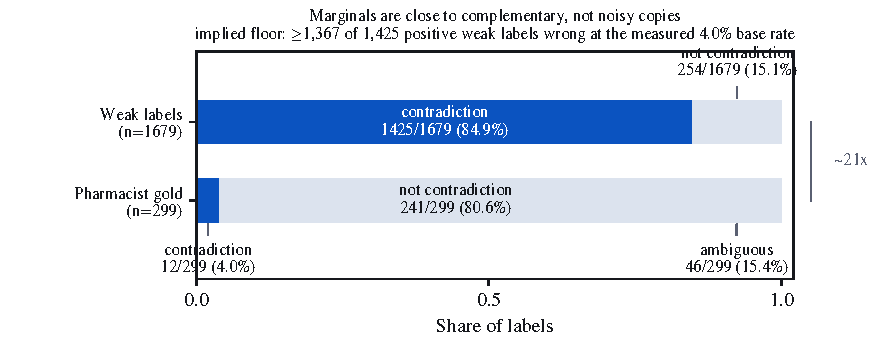
\includegraphics[width=0.92\linewidth]{figures/fig-prevalence.pdf}
\caption{The prevalence mismatch. The reader should notice that the two
distributions are not noisy versions of each other; they are close to
complementary. No aggregation or noise-robust loss recovers a correct
conditional from supervision whose marginal is inverted.}
\label{fig:prevalence}
\end{figure}

\begin{figure}[t]
\centering
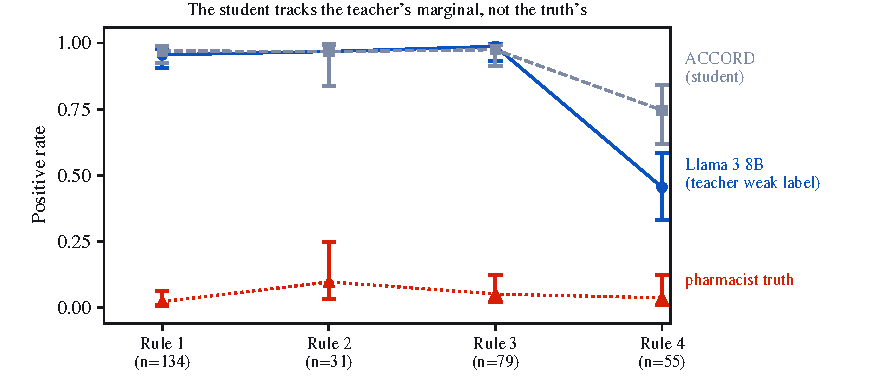
\includegraphics[width=0.92\linewidth]{figures/fig-tracking.pdf}
\caption{Marginal transfer from teacher to student. On Rules 1 to 3 the student's
positive rate is within $1.5$ points of the teacher's while true prevalence
varies fourfold across the same rules. On Rule 4, where the teacher is
genuinely selective, the student regresses towards its own global prior rather
than inheriting the selectivity.}
\label{fig:tracking}
\end{figure}

\section{Limitations}
\label{sec:weak-limitations}

\paragraph{One labeller.} Every conclusion in this chapter concerns Llama 3 8B
under one prompt. Whether a larger model, a different prompt, a chain-of-thought
format, or a calibrated decision rule would behave differently is untested here.
Chapter~\ref{ch:eval} reports a GPT-4o comparison on the gold set only, which is
suggestive but not a weak-supervision experiment.

\paragraph{A related model-agnostic claim in this project is withdrawn.} An
earlier project artifact reported that clinical miscalibration was
``model-agnostic'' on the basis of two models. Only one of the two loaded; the
second returned an authorisation failure on every run, and its row in the
results table was a hardcoded literal. The claim rests on one model and is
retracted. It is mentioned here because the same failure default, scoring
unparseable generations as positive, appears in that component, and is the basis
of the [TODO] in Section~\ref{sec:weak-acquiescence}.

\paragraph{The base rate is measured on $299$ pairs with $12$ positives.} The
$4.0\%$ figure has a wide confidence interval. The $21\times$ ratio would remain
large under any plausible interval, but it should not be quoted to more than one
significant figure.

\paragraph{The exemplar defect confounds the weak labels in the same way it
confounds the gold labels.} The labeller saw the same $41.4\%$-contaminated
exemplars. Unlike the gold labels, however, the weak labels are not used as
ground truth anywhere in this thesis; they are used only as training
supervision, and the claim made about them, that their marginal is wrong by
$21\times$, does not depend on which sentences were shown.

\paragraph{No attempt was made to correct the mismatch.} Prior correction,
threshold shifting, class-balanced resampling, and positive-unlabelled learning
are all standard responses to a known prior shift, and none was tried. This is a
gap in the work, not evidence that they would have failed.
Chapter~\ref{ch:eval}'s threshold sweep bears on this: the model's scores carry
no ranking signal at all, so post-hoc threshold correction has nothing to work
with. That is an argument that correction would not have sufficed \emph{here},
not that prior correction is generally ineffective.

\section{Summary}
\label{sec:weak-summary}

An instruction-tuned language model labelled $1{,}679$ candidate pairs and
called $84.9\%$ of them contradictions against a measured base rate of $4.0\%$.
At least $95\%$ of its positive labels are false positives. The detector trained
on those labels reproduces the labeller's per-rule positive rate to within
$1.5$ percentage points on three of four rules, while the rules' true
prevalences differ from one another by more than a factor of four, which is the
signature of a model that has learned the label's marginal rather than its
conditional. On the one rule where the labeller was genuinely selective, the
student regressed towards its own prior instead of inheriting the distinction.

The confidence field accompanying the weak labels takes two values and is a
deterministic function of the label. It was used both as a filter, where it
removed nothing, and as a per-example loss weight, where it silently reweighted
by class.

The whole failure is detectable before training, with a base-rate estimate, a
printed marginal, a distinct-value count, and a direct comparison against the
human labels that were already available. Chapter~\ref{ch:arch} turns to the
model that consumed these labels, and to three architectural claims that do not
survive contact with the code that produced them.

% ============================================================================
%  Chapter 6. Architecture, and the Falsification of Three Claimed Contributions
%
%  \input file. Requires booktabs, amsmath, natbib in the parent preamble.
%  Bibliography: accord/thesis/refs.bib
%
%  Traceability: accord/CORRECTIONS.md C1, C2, C4, C5, C7, C8;
%  accord_phase3_v2_ablations.py; transfer_results_correct.json;
%  the Stage 0 pretraining logs.
% ============================================================================

\chapter{Architecture, and the Falsification of Three Claimed Contributions}
\label{ch:arch}

\section{What This Chapter Does}
\label{sec:arch-overview}

The preceding chapters concerned data and supervision. This chapter concerns the
model, and it is written in an unusual form: as a falsification report. ACCORD
was specified with four purpose-built components layered over a biomedical
encoder, and three claimed contributions were attached to them. An audit of the
code that produced the reported results establishes that none of the three
survives.

\begin{enumerate}
\item \textbf{Claimed:} the model discovers clinical note priority without
      supervision, converging to weights $\alpha_N \approx 0.5$,
      $\alpha_D \approx 1.0$. \textbf{Actual:} the parameter is
      \emph{initialised} at exactly $[0.5, 1.0]$ and moves by $1.8\%$ and
      $0.6\%$ across seeds. Section~\ref{sec:c1}.
\item \textbf{Claimed:} an auxiliary rule-type head reaches $F_1 = 0.9603$,
      evidencing pharmacologically grounded structure. \textbf{Actual:} the rule
      identifier is written into the model's input features and predicted in the
      same forward pass, one linear layer away. Section~\ref{sec:c2}.
\item \textbf{Claimed:} guideline-grounded harm estimation produces ranked
      danger scores. \textbf{Actual:} the guideline bank is twenty random
      vectors, and the harm head receives no loss term at any point in training.
      Section~\ref{sec:c3}.
\end{enumerate}

A fourth finding, the collapse of self-supervised pretraining to the
constant-prediction solution, is reported in Section~\ref{sec:stage0} together
with a retraction of the explanation originally given for it.

The chapter closes with the constructive residue: a set of diagnostics, each
costing a few lines of code, any one of which would have caught the
corresponding failure before it reached a results table.

\section{Backbone and Adaptation}
\label{sec:backbone}

The encoder is BioMedBERT \citep{gu2021biomedbert}, a $110$M-parameter
transformer pretrained from scratch on PubMed abstracts and full texts. It was
selected over ClinicalBERT \citep{alsentzer2019clinicalbert} on the basis of
published benchmark performance; that choice is defensible and is not among the
findings of this chapter.

Adaptation uses LoRA \citep{hu2022lora} with rank $r = 16$ and
$\alpha = 32$ on the attention projections. Chapter~\ref{ch:eval} reports the
one place in this project where the backbone and the adapter were evaluated
correctly, on MedNLI \citep{romanov2018mednli}, and the result there is sound.
It is also, as that chapter argues at length, a result about BioMedBERT, not
about ACCORD.

Input construction: each candidate's nursing sentence and discharge sentence are
encoded, each truncated to $256$ WordPiece tokens taken from the head of the
sequence. Section~\ref{sec:stage0} returns to that truncation.

\section{The Specified Architecture}
\label{sec:spec}

\begin{table}[t]
\centering
\small
\begin{tabular}{llr}
\toprule
\textbf{Component} & \textbf{Stated function} & \textbf{Params} \\
\midrule
CDE  & [TODO: expand acronym from the original specification] & 527,104 \\
ATCG & [TODO: expand acronym from the original specification] & 395,269 \\
PPC  & Pharmacological Prior Conditioning: injects drug-class, & 2,496 \\
     & interaction, and contraindication priors & \\
GGHE & Guideline-Grounded Harm Estimation: retrieval-augmented & 614,916 \\
     & harm scoring against published HF guidelines & \\
\midrule
     & \textbf{Total new parameters (v1 specification)} & \textbf{1,539,785} \\
\bottomrule
\end{tabular}
\caption{The specified architecture, as described in the project's own
documentation. Two acronym expansions are not recoverable from surviving
artifacts and are marked [TODO] rather than reconstructed. The total,
$\approx 1.54$M, is the figure quoted throughout the project's writeups.
Section~\ref{sec:actual} establishes that this table describes v1 and that no
reported result was produced by v1.}
\label{tab:spec}
\end{table}

Table~\ref{tab:spec} is what the project claimed to have built. The parameter
counts are internally consistent and sum to the quoted $1.54$M. The problem is
not arithmetic.

\section{The Architecture That Actually Ran}
\label{sec:actual}

\begin{table}[t]
\centering
\small
\begin{tabular}{p{0.24\linewidth}p{0.68\linewidth}}
\toprule
\textbf{Claimed} & \textbf{Actual, in the code that produced the results} \\
\midrule
PPC, $2{,}496$ params, injects pharmacological priors
& \textbf{Deleted in v2.} Replaced by a function \texttt{\_prior()} returning a
  $64$-dimensional vector of zeros with two positions overwritten:
  \texttt{pf[i,0]} $=$ a danger multiplier and \texttt{pf[i,1]} $=$
  \texttt{rule/4.0}. \textbf{Zero learned parameters.} No drug class, no
  interaction table, no contraindication list. \\
\addlinespace
GGHE, retrieval-augmented scoring against published HF guidelines
& A single \texttt{nn.Parameter(torch.randn(20, 256))}: twenty random vectors,
  cross-attended from one query. No corpus, no index, no retrieval, no guideline
  text. The code comment reads \emph{``In full version this attends over
  FAISS-retrieved chunks.''} \\
\addlinespace
Guideline-grounded harm estimation produces ranked danger scores
& \texttt{harm\_head} and \texttt{explanation\_head} \textbf{receive no loss
  term}. The total objective is
  $\mathcal{L} = 1.0\,\mathcal{L}_{\text{contra}} + 0.3\,\mathcal{L}_{\text{rule}}$.
  Neither head appears in it. \\
\addlinespace
$1.54$M new parameters
& Describes v1. v2 adds an \texttt{AsymmetricCrossNoteEncoder}: two $8$-head,
  $768$-dimensional multi-head attention blocks plus two $768 \times 768$
  projections, $\approx 5.9$M parameters, and removes PPC's $2{,}496$. The model
  that produced every reported result carries $\approx 7.5$M new parameters, not
  $1.54$M. \\
\bottomrule
\end{tabular}
\caption{Specification against implementation. The right column is what the
code does. Every result reported in this thesis, and every result reported in
the project's earlier writeups, was produced by the right column.}
\label{tab:actual}
\end{table}

Table~\ref{tab:actual} should be read as a whole rather than component by
component, because the pattern matters more than any single row. In each case
a component was specified, a placeholder was written so that the surrounding
code would run, and the placeholder was never replaced. The pipeline executed
end to end, produced numbers, and those numbers were reported against the
specification rather than against the placeholder. Nothing in the codebase
compared the two.

This is the structural failure of the project. It is a documented failure mode
of machine learning systems \citep{sculley2015debt}, and the remedy is
mechanical: a model summary printed at training time, listing every module, its
parameter count, and whether it appears in the loss graph.
Section~\ref{sec:diagnostics} states it as a protocol.

\section{Falsification 1: Authority Conditioning Is an Initialisation Artifact}
\label{sec:c1}

\subsection{The claim}

The project's third stated contribution was that ACCORD recovers clinical note
priority without ever being told it. Specifically: without explicit authority
labels, the model's authority weights converge to the correct clinical
hierarchy, $\alpha_N \approx 0.5$ for nursing and $\alpha_D \approx 1.0$ for
discharge. This was presented as evidence that institutional note priority is
learnable from weak supervision alone.

\subsection{The code}

\begin{quote}\ttfamily\small
def \_\_init\_\_(self, hidden\_size=768, num\_heads=8, dropout=0.1,
authority\_dampening=0.5): \\
\hphantom{def }self.authority\_scale = nn.Parameter(torch.tensor([authority\_dampening, 1.0]))
\end{quote}

The parameter is initialised at exactly $[0.5, 1.0]$: the values reported as
discovered.

\subsection{The measurement}

Across three seeds the parameter moved to $(0.509, 1.006)$, relative changes of
$1.8\%$ and $0.6\%$. Third-decimal agreement across independent seeds is not the
signature of a recovered signal. It is the signature of a parameter that did not
train.

\subsection{The mechanism}

The scale is applied to a cross-attention branch that is immediately
LayerNorm'd. LayerNorm is invariant to a per-branch scalar rescaling of its
input up to the effect on its own learned affine parameters, so the normalisation
removes most of what the authority scale does, and the gradient flowing back to
it is correspondingly near zero. The parameter is not merely uninformative; it
is architecturally prevented from mattering.

\subsection{The project's own ablation already refuted the claim}

The clearest evidence was present in the results table and was not read. A
symmetric variant, with $\alpha_N = \alpha_D$, \emph{outperforms} the full
asymmetric model:

\begin{table}[h]
\centering
\small
\begin{tabular}{lrr}
\toprule
 & \textbf{Contradiction $F_1$} & \textbf{Accuracy} \\
\midrule
Symmetric (constrained $\alpha_N = \alpha_D$) & \textbf{0.7775} & \textbf{0.9192} \\
Full asymmetric model                          & 0.7368 & 0.8939 \\
\bottomrule
\end{tabular}
\caption{The asymmetry ablation. Removing the mechanism claimed as a
contribution improves both reported metrics. Both rows are measured against
\emph{weak} labels on the held-out split, not against pharmacist labels, so they
describe agreement with an $84.9\%$-positive teacher rather than clinical
correctness. [TODO: report the majority-class baseline on this exact split.
Without it, an $F_1$ of $0.7775$ against supervision that is $84.9\%$ positive
cannot be interpreted, because a constant-positive predictor achieves a high
$F_1$ by construction under that marginal.]}
\label{tab:acne}
\end{table}

\subsection{What should be reported instead}

The claim is retracted in full. Its replacement is the diagnostic that would
have caught it, stated as a general rule: \emph{for any parameter reported as
learned, publish $\lVert\theta_{\text{final}} - \theta_{\text{init}}\rVert /
\lVert\theta_{\text{init}}\rVert$ and a gradient-norm trace.} Applied here,
those two quantities are $1.8\%$/$0.6\%$ and approximately zero, and the claim
does not survive its own first diagnostic.

\subsection{What this does not establish}

It does not establish that clinical note priority is unlearnable, nor that
asymmetric conditioning is a bad idea. It establishes that this implementation
did not test the hypothesis. The hypothesis remains open, and a correct test
would require a parameter placed outside a normalisation that erases it, an
initialisation that does not encode the expected answer, and a measurement of
displacement from that initialisation.

\section{Falsification 2: The Rule-Type Head Is Label Leakage}
\label{sec:c2}

\subsection{The claim}

A multi-task auxiliary head predicts which of the four rules generated a
candidate, reaching $F_1 = 0.9603$ (reported as $0.953 \pm 0.006$ in the
project's ablation table). This was offered as evidence that the model learns
pharmacologically grounded structure rather than surface cues.

\subsection{The code}

The prior-feature constructor writes the rule identifier into the model's input:

\begin{quote}\ttfamily\small
pf[i, 1] = rule / 4.0\hfill\# rule comes from the batch \\
\ldots \\
return self.gghe(edge\_repr, prior) \\
rule\_logits = self.rule\_type\_head(attended)\hfill\# predicts RULE\_MAP[rule]
\end{quote}

The auxiliary label is an input feature and the prediction target in the same
forward pass, separated by one linear layer. The task is a copy operation, and
$F_1 = 0.9603$ is the accuracy of that copy.

\subsection{The independent confirmation}

Leakage of this kind is invisible in domain and unmistakable out of domain,
because the leaked feature is present in both cases but the surface correlations
supporting a genuine solution are not. Table~\ref{tab:transfer} reports the
transfer test.

\begin{table}[t]
\centering
\small
\begin{tabular}{lr}
\toprule
\textbf{Setting} & \textbf{Rule-type $F_1$} \\
\midrule
Heart failure (in domain) & 0.9603 \\
Sepsis (transfer)         & 0.0654 \\
AKI (transfer)            & 0.0595 \\
\midrule
Rule-prediction accuracy on the held-out pharmacist set & 45.2\% \\
\bottomrule
\end{tabular}
\caption{Rule-type prediction in domain and under transfer. A head reaching
$0.96$ in domain collapses to $0.065$ and $0.060$ on two other ICD-9 cohorts
drawn from the same institution, the same note types, the same extractor, and
the same four rules. A drop of that magnitude between populations that differ
only in index diagnosis is not distribution shift in any ordinary sense. It is
the removal of whatever the head was actually using.}
\label{tab:transfer}
\end{table}

The transfer collapse is the better number to report, and it is reported here in
place of $0.9603$, which is withdrawn. It is the \emph{evidence} of the leakage
rather than an embarrassment to be minimised, and it happens to answer the
generalisation question directly: this model does not transfer between clinical
cohorts.

\subsection{Positioning}

Auxiliary-label leakage of this shape belongs to a well-documented family. NLI
models exploit hypothesis-only artifacts \citep{poliak2018hypothesis,
gururangan2018artifacts} and syntactic heuristics \citep{mccoy2019hans};
radiology models key on hospital-identifying image features and collapse across
sites \citep{zech2018generalization}; the general phenomenon is shortcut
learning \citep{geirhos2020shortcut}. The contribution of this section is not
the observation that shortcuts exist. It is the specific, checkable point that
\emph{an auxiliary head whose target is derivable from the input features is not
an auxiliary task}, and that the cheapest test for it is out-of-domain transfer,
not held-out accuracy.

\section{Falsification 3: Harm Estimation Was Never Trained}
\label{sec:c3}

\subsection{The claim}

The project posed a research question about guideline-grounded severity ranking:
whether contradictions can be ordered by clinical danger using evidence from
published heart-failure guidelines. GGHE was the component that would answer it.

\subsection{The code}

Three facts, each independently sufficient.

\paragraph{There is no guideline corpus.} The ``guideline bank'' is
\texttt{nn.Parameter(torch.randn(20, 256))}. Twenty vectors, drawn from a
standard normal at initialisation, cross-attended from a single query. There is
no document collection, no index, no retrieval step, and no text of any kind. The
code comment states that a full version would attend over retrieved chunks; that
version does not exist.

\paragraph{The harm head receives no gradient.} The total objective is
$\mathcal{L} = 1.0\,\mathcal{L}_{\text{contra}} +
0.3\,\mathcal{L}_{\text{rule}}$. The harm head and the explanation head are not
in it. They are randomly initialised modules whose outputs are computed,
recorded, and reported, and whose weights never move.

\paragraph{The outputs are consistent with an untrained sigmoid.} Across the
$299$ gold pairs, harm scores span $0.398$ to $0.610$: a narrow band centred on
$0.5$, which is what a randomly initialised head produces. The derived
high-risk rate is $0.0$ in all three cohorts, because no score ever crosses the
threshold.

\subsection{Consequence}

\textbf{The severity-ranking research question was not tested.} The component
that would have answered it was never trained, and the scores it emits are
random-initialisation noise. Chapter~\ref{ch:eval} reports the corresponding
empirical result, a Spearman correlation between harm score and pharmacist
danger rating of $-0.0001$ at $p = 0.999$, which is as close to a pure null as a
finite sample produces. That number is not a negative finding about severity
ranking. It is a measurement of an untrained module, and it should be read as
confirming Section~\ref{sec:c3} rather than as evidence about the underlying
question.

Stating this correctly matters more than it might appear. A reader encountering
$\rho = -0.0001$ without this section would reasonably conclude that clinical
severity is not predictable from these features. The correct conclusion is that
nothing was asked of the model.

\section{The Stage 0 Collapse}
\label{sec:stage0}

\subsection{The setup}

Before supervised training, ACCORD was to be pretrained with a self-supervised
cross-note coherence objective: discriminate genuine (nursing, discharge) pairs
from mismatched pairs, on the theory that a representation able to tell a real
pairing from a fake one has learned something about cross-note consistency.

\subsection{The result}

The objective converged to exactly $\ln 2 = 0.693$ with development accuracy of
$0.5000$ at every epoch. This is the constant-prediction solution: binary
cross-entropy at $p = 0.5$ for every example. The model learned to emit a
constant.

Critically, this held in \emph{both} training configurations:

\begin{table}[h]
\centering
\small
\begin{tabular}{lrrr}
\toprule
\textbf{Configuration} & \textbf{Trainable params} & \textbf{Final loss} & \textbf{Dev acc.} \\
\midrule
Frozen backbone             & 592,647    & 0.693 ($=\ln 2$) & 0.5000 \\
Partially unfrozen backbone & 22,446,855 & 0.693 ($=\ln 2$) & 0.5000 \\
\bottomrule
\end{tabular}
\caption{Stage 0 coherence pretraining. Increasing trainable capacity by a
factor of $37.9$ changes nothing. Identical collapse under wildly different
capacity is strong evidence that the constraint is architectural or
representational, not a matter of insufficient parameters or optimisation
budget.}
\label{tab:stage0}
\end{table}

\subsection{A retracted explanation}

The original diagnosis was that clinical notes within an institution are too
homogeneous for a coherence objective to separate real from mismatched pairs.
\textbf{This explanation is withdrawn.} Nothing in the pipeline measured note
similarity, within an admission or between admissions. No embedding distance, no
lexical overlap statistic, no discriminability estimate was computed. The
explanation was asserted, it was plausible, and it was never tested. It is
withdrawn not because it is known to be false but because there is no evidence
for it, and an untested causal story attached to a null result is the most
easily propagated kind of error.

\subsection{Two mechanisms that are visible in the code}

Two properties of the implementation are directly observable and are each
sufficient to produce the observed collapse. Neither was isolated
experimentally, and the language here is chosen to reflect that.

\paragraph{A one-dimensional bottleneck.} The scoring path is
\texttt{conflict\_scorer} $\rightarrow$ \texttt{sigmoid} $\rightarrow$
\texttt{Linear(1,1)}. The entire pair representation is compressed to a single
scalar, squashed into $(0,1)$, and then passed through an affine map of one
parameter. Three consequences follow. The model can express only a monotone
function of one scalar, so any structure requiring two or more directions is
unrepresentable. The sigmoid sits between the representation and the loss, so
whenever the scalar drifts into a saturated region the gradient reaching
everything upstream is attenuated. And a scalar that collapses to a constant
produces a constant output regardless of how much capacity sits behind it, which
is exactly the invariance observed in Table~\ref{tab:stage0}.

\paragraph{Head truncation into the de-identification header.} Each note is
truncated to its first $256$ WordPiece tokens, taken from the head. As
Chapter~\ref{ch:data} noted, the head of a MIMIC-III discharge summary is the
administrative header block, where de-identification surrogates are densest. For
a substantial fraction of pairs the model is discriminating between two
administrative headers, which carry no information about whether the pairing is
genuine. A model given inputs that do not contain the discriminating signal
correctly learns to predict the base rate, and the base rate of a balanced
real-versus-mismatched task is exactly $0.5$.

\paragraph{The experiments that would separate them.} [TODO: (a) widen the
bottleneck from $d = 1$ to $d \in \{64, 256\}$ and rerun Stage 0, holding
everything else fixed; (b) hold the bottleneck fixed and replace head truncation
with truncation centred on a medication-bearing sentence, and rerun; (c) report
the fraction of truncated discharge-summary windows containing at least one
extracted medication mention, which bounds how often the input can possibly
carry signal.] Item (c) costs minutes and should be done first.

\section{Experimental Hygiene}
\label{sec:hygiene}

Three further defects concern how experiments were run rather than what was
built. They are reported because they bear on how much weight any reported
number can carry.

\subsection{Training on the evaluation set}

One reported configuration trained on the full $1{,}978$-pair pool, which
contains the $299$ pharmacist-annotated pairs used for evaluation. Results from
that configuration are not reported anywhere in this thesis. Any earlier project
artifact quoting them should be treated as superseded. The only reported
configuration is the one trained on the held-out complement.

\subsection{Seeds}

The ablation table reports three seeds with a standard deviation. In the code,
\texttt{SEEDS = [1, 2]}. The third row is a pasted literal from an earlier run at
a different code state. Further, \texttt{set\_seed()} is never called inside the
training loop, so each ablation variant inherits whatever RNG state the previous
variant left behind, making the variants sequentially dependent. The data split
uses \texttt{random\_state=42} in every case, so the reported $\pm$ reflects
initialisation noise only and contains no sampling variance whatever.

A separate problem compounds this: the full-model reference row in the ablation
table is itself a hardcoded literal. \textbf{The full model is not run by the
ablation script.} The table therefore compares three freshly trained variants
against a pasted reference, which means the differences it reports are not
differences measured under a common protocol. The ablation table should be
regenerated. Until it is, the only defensible reading of
Table~\ref{tab:acne} is directional.

\subsection{Row-level splits}

The reference pipeline split the candidate pool at the row level, as
Chapter~\ref{ch:candidates} documented: $1{,}978$ pairs drawn from $1{,}203$
admissions, roughly $1.64$ per admission, in a population with known repeat
admissions. Pairs sharing a nursing note, a discharge summary, or a patient
routinely land on both sides. The rebuild splits by patient with disjointness
asserted in code.

\subsection{The cumulative effect}

Taken together these mean that the ablation numbers in this chapter,
including Table~\ref{tab:acne}, should be read as descriptive rather than
inferential. They are reported because the qualitative pattern they show,
symmetric beating asymmetric, is informative regardless of the error bars. No
significance claim is made on any of them.

\section{A Diagnostic Protocol}
\label{sec:diagnostics}

The constructive contribution of this chapter is that each failure has a cheap,
mechanical detector, and that all of them belong in the training loop rather
than in a post-hoc audit. The protocol below is stated generally and each item
is annotated with the failure it catches.

\begin{enumerate}
\item \textbf{Print a module manifest at training time}: every named module,
      its parameter count, and a boolean indicating whether it appears in the
      autograd graph of the loss. \emph{Catches:} the PPC deletion, the
      untrained harm and explanation heads, and the $1.54$M-versus-$7.5$M
      parameter discrepancy (Section~\ref{sec:actual}).
\item \textbf{For every parameter reported as learned, log
      $\lVert\theta_{\text{final}} - \theta_{\text{init}}\rVert /
      \lVert\theta_{\text{init}}\rVert$ and a gradient-norm trace.}
      \emph{Catches:} the authority-conditioning artifact
      (Section~\ref{sec:c1}).
\item \textbf{For every auxiliary head, assert that its target is not derivable
      from its input features}, and verify by transfer rather than by held-out
      accuracy. \emph{Catches:} the rule-type leakage
      (Section~\ref{sec:c2}).
\item \textbf{Report a majority-class baseline alongside every $F_1$}, computed
      on the exact split being reported. \emph{Catches:} the uninterpretability
      of Table~\ref{tab:acne} under $84.9\%$-positive supervision.
\item \textbf{Assert group disjointness of splits in code}, at the coarsest
      grouping unit present in the data (here, patient). \emph{Catches:} the
      row-level split.
\item \textbf{Assert that the evaluation set is absent from the training set},
      by identifier, at load time. \emph{Catches:} the contaminated
      configuration.
\item \textbf{Call the seed setter inside the loop, not outside it}, and refuse
      to emit a standard deviation over fewer than three genuinely independent
      runs. \emph{Catches:} the seed reporting.
\item \textbf{Report the empirical range of every score the model emits.} A
      score spanning $0.398$ to $0.610$ across a full evaluation set is the
      range of an untrained sigmoid and should stop a results table.
      \emph{Catches:} the harm head (Section~\ref{sec:c3}).
\item \textbf{Run a transfer evaluation on any cohort at all before claiming
      generalisation.} \emph{Catches:} both the rule leakage and any surface
      memorisation.
\end{enumerate}

Every one of these is standard practice somewhere. None of them was in this
pipeline. The claim being made is not that they are novel; it is that their
absence is what allowed four separate unsupported claims to reach a submission,
and that a project of this shape should treat them as non-optional
instrumentation rather than as good hygiene.

\section{Proposed Figures}
\label{sec:arch-figures}

\begin{figure}[t]
\centering
\framebox[\linewidth]{\parbox[c][6cm][c]{0.92\linewidth}{\centering
\textit{[Figure asset 6.1: two-column architecture diagram. Left column,}
\textit{``as specified'': BioMedBERT $\rightarrow$ CDE $\rightarrow$ ATCG}
\textit{$\rightarrow$ PPC $\rightarrow$ GGHE $\rightarrow$ \{contradiction,}
\textit{rule, harm, explanation\} heads, with the 1.54M total. Right column,}
\textit{``as implemented'': the same skeleton with PPC struck through and}
\textit{replaced by a zero vector box, GGHE's bank annotated}
\textit{``randn(20,256)'', the harm and explanation heads greyed out and}
\textit{labelled ``no loss'', ACNE added at 5.9M, total 7.5M. Loss graph edges}
\textit{drawn only for the two heads that receive gradient.]}}}
\caption{Specification against implementation. The reader should notice that the
two heads carrying the project's severity and explainability claims are not
connected to the loss, and that the parameter budget is off by a factor of
roughly five in the opposite direction from what the writeups claim.}
\label{fig:arch}
\end{figure}

\begin{figure}[t]
\centering
\framebox[\linewidth]{\parbox[c][5cm][c]{0.92\linewidth}{\centering
\textit{[Figure asset 6.2: two panels. Left, a bar pair for the authority}
\textit{parameter: initialisation (0.5, 1.0) against final (0.509, 1.006),}
\textit{with the relative displacement annotated as 1.8\% and 0.6\%, plus a}
\textit{gradient-norm trace inset that is flat near zero. Right, rule-type F1}
\textit{across three cohorts: HF 0.9603, sepsis 0.0654, AKI 0.0595, with the}
\textit{45.2\% held-out rule accuracy marked as a horizontal reference.]}}}
\caption{The two falsifications in one view. Left: a parameter reported as
learned that did not move. Right: a head reported at $F_1 = 0.96$ that retains
nothing outside its training cohort. Both diagnostics are one line of code and
neither was run before the claims were made.}
\label{fig:falsification}
\end{figure}

\section{Limitations of This Chapter}
\label{sec:arch-limitations}

\paragraph{This is an audit, not a controlled study.} The falsifications are
established by reading code and by measurements already present in the run
artifacts. They establish that the claims were unsupported. They do not
establish what a correct implementation of any of the four components would do,
and this thesis makes no claim about that.

\paragraph{The Stage 0 mechanisms are hypotheses supported by code reading, not
by ablation.} Section~\ref{sec:stage0} is explicit about this and lists the
experiments that would separate them. The strongest evidence available is the
invariance across a $37.9\times$ capacity change, which rules out capacity but
does not adjudicate between the bottleneck and the truncation.

\paragraph{The transfer collapse has an alternative reading.} A drop from $0.96$
to $0.065$ is consistent with leakage plus genuine cohort shift, and the two are
not separated here. The candidate rules, the drug dictionary, and the class
dictionary are all heart-failure specific, so the sepsis and AKI candidate pools
differ in composition as well as in surface features. The leakage claim rests
primarily on the code, in which the rule identifier is an input feature; the
transfer number corroborates it rather than proving it alone.
[TODO: run the direct ablation, zero out \texttt{pf[i,1]} at inference and
re-measure in-domain rule $F_1$. If it collapses, the leakage claim is closed.]

\paragraph{The ablation numbers carry no valid error bars.}
Section~\ref{sec:hygiene}. They are reported directionally and no significance
claim is attached to any of them.

\paragraph{No comparison against a simple baseline architecture.} The project
never trained a plain BioMedBERT sentence-pair classifier on the same weak
labels and the same splits. That is the single most important missing
experiment in this chapter, because it would establish how much of the reported
behaviour is attributable to the custom components at all.
[TODO: train a vanilla cross-encoder baseline on the identical held-out split
and report it alongside every ACCORD row.]

\section{Summary}
\label{sec:arch-summary}

ACCORD was specified as a biomedical encoder plus four purpose-built components
totalling $1.54$M parameters. The model that produced every reported result
contains roughly $7.5$M new parameters, is missing one of the four components
entirely, and connects only two of its four output heads to the loss.

Three claimed contributions are falsified. The authority weights reported as
discovered were the initialisation values, displaced by under two percent, on a
branch that a subsequent LayerNorm largely erases; the project's own ablation
shows that removing the asymmetry improves both reported metrics. The
rule-type head's $F_1$ of $0.9603$ is a copy of an input feature, and it
collapses to $0.0654$ and $0.0595$ on two transfer cohorts and to $45.2\%$
accuracy on the held-out annotated set. Guideline-grounded harm estimation was
never trained: its guideline bank is twenty random vectors and its head is
absent from the loss, so its output range of $0.398$ to $0.610$ is the range of
an untrained sigmoid and the associated research question was not tested.

Self-supervised pretraining converged to the constant-prediction solution, at
$\ln 2$ with development accuracy exactly $0.5000$, identically under a
$37.9\times$ change in trainable capacity. The explanation originally given for
this, that clinical notes are too homogeneous, is withdrawn as untested. Two
mechanisms are visible in the code: a one-dimensional scoring bottleneck and
head truncation into the de-identification block.

Chapter~\ref{ch:eval} measures what this model does on the pharmacist-annotated
set, four independent ways, and finds that its scores contain no information
about the labels.

% ============================================================================
%  Chapter 7. Evaluation: Four Independent Measurements of Failure
%
%  \input file. Requires booktabs, amsmath, natbib in the parent preamble.
%  Bibliography: accord/thesis/refs.bib
%
%  Traceability: the audit scripts over the 299 pharmacist-annotated pairs,
%  transfer_results_correct.json, the MedNLI fine-tuning logs, and
%  accord/CORRECTIONS.md (C2, C4, C5).
% ============================================================================

\chapter{Evaluation: Four Independent Measurements of Failure}
\label{ch:eval}

\section{Evaluation Design}
\label{sec:eval-design}

A negative result is only worth reporting if it is difficult to escape. A single
unfavourable metric invites the response that the metric was the wrong one, the
threshold was badly chosen, the class balance was hostile, or the sample was too
small. This chapter is constructed to make those responses unavailable, by
measuring the same system four ways that fail for different reasons if they fail
at all.

\begin{enumerate}
\item \textbf{Ranking.} Does the model's contradiction probability order the
      pharmacist's labels better than chance? This is threshold-free and
      insensitive to class balance. Section~\ref{sec:m1}.
\item \textbf{Operating points.} Is there \emph{any} threshold at which the
      model is usable? This removes the objection that $0.5$ was the wrong
      cut. Section~\ref{sec:m2}.
\item \textbf{Severity.} Does the model's harm score correlate with the
      pharmacist's $1$ to $5$ danger rating? This asks a different question of a
      different output head. Section~\ref{sec:m3}.
\item \textbf{Comparison.} How does the model rank against a general-purpose
      language model, zero-shot and few-shot, and against the weak labeller it
      was distilled from, on the same $299$ pairs? This removes the objection
      that the task is simply impossible. Section~\ref{sec:m4}.
\end{enumerate}

All four are computed on the $299$ pharmacist-annotated pairs, which are absent
from the training set by construction (Chapter~\ref{ch:weak},
Section~\ref{sec:weak-setup}). The single configuration that trained on those
pairs is not reported anywhere in this thesis.

Section~\ref{sec:eval-scoping} then addresses the obvious objection: given the
exemplar defect of Chapter~\ref{ch:candidates}, can any of this be believed? The
answer is a qualified yes, and the qualification is stated precisely rather than
waved at.

\section{A Component Sanity Check: BioMedBERT on MedNLI}
\label{sec:mednli}

\subsection{Purpose}

Before reporting that a system fails, it is worth establishing that the pieces
were assembled competently. MedNLI \citep{romanov2018mednli} is the standard
clinical natural language inference benchmark: premise and hypothesis pairs derived
from MIMIC-III, labelled entailment, contradiction, or neutral. It is the
closest well-established task to the one this thesis attempts, and it has an
established performance range.

\subsection{Result}

\begin{table}[t]
\centering
\small
\begin{tabular}{lrrr}
\toprule
\textbf{Configuration} & \textbf{Trainable} & \textbf{Test acc.} & \textbf{Macro $F_1$} \\
\midrule
BioMedBERT, full fine-tune, 10 epochs        & full backbone & 83.90\% & 83.91\% \\
BioMedBERT $+$ LoRA ($r{=}16$, $\alpha{=}32$), 5 epochs & 592,131 & 72.93\% & 72.74\% \\
\midrule
Published range for comparable systems       & n/a & \multicolumn{2}{c}{83 to 87\%} \\
\bottomrule
\end{tabular}
\caption{MedNLI results. The full fine-tune sits inside the published range for
comparable encoder-based systems. This establishes that the backbone, the
tokenisation, the training loop, and the evaluation harness are sound. The LoRA
configuration used for ACCORD loses roughly eleven accuracy points, which is a
material cost that was not accounted for in the project's design.}
\label{tab:mednli}
\end{table}

\subsection{What this row is, and what it is not}

\textbf{Table~\ref{tab:mednli} is a BioMedBERT baseline. It is not ACCORD.} Zero
ACCORD components are present in either model: no cross-note encoder, no
authority conditioning, no prior conditioning, no harm estimation. It is a
sentence-pair classifier on a public benchmark.

This distinction is emphasised because the alternative framing, reporting
$83.90\%$ under the project's own system name, would be the single most
misleading move available in this thesis. A reader encountering
``ACCORD: $83.9\%$ on MedNLI'' followed by the results in
Section~\ref{sec:eval-point} would reasonably conclude that a strong model
failed on a hard task. What actually happened is that a strong \emph{backbone}
performs as expected on a benchmark it was designed for, and a differently
constructed system built on that backbone fails on a different task for reasons
that have nothing to do with the backbone's capability.

\subsection{One substantive finding}

The eleven-point gap between full fine-tuning and LoRA is worth recording. LoRA
is often described as approximately loss-free relative to full fine-tuning
\citep{hu2022lora}, and on many tasks it is. Here, at $r = 16$ with $592{,}131$
trainable parameters and a shorter schedule, it is not. ACCORD used the LoRA
configuration. Whether the gap reflects rank, schedule length, or the specific
demands of clinical inference is untested here. [TODO: run a rank sweep
$r \in \{8, 16, 64, 256\}$ at matched epochs on MedNLI and report the
accuracy and parameter frontier. The two rows in Table~\ref{tab:mednli} differ in
both rank and schedule and therefore do not isolate either.]

\section{Point Metrics on the Gold Set}
\label{sec:eval-point}

\begin{table}[t]
\centering
\small
\begin{tabular}{lr}
\toprule
\textbf{Quantity} & \textbf{Value} \\
\midrule
Annotated pairs                                   & 299 \\
\quad true contradictions                         & 12 \\
\quad not contradictions                          & 241 \\
\quad ambiguous                                   & 46 \\
\midrule
Pairs ACCORD predicts \emph{contradiction} at $\tau = 0.5$ & 278 \\
\midrule
Precision                                         & 0.047 \\
Recall                                            & 0.917 (11/12) \\
Accuracy                                          & 0.115 \\
Pooled base rate                                  & 0.040 (12/299) \\
\bottomrule
\end{tabular}
\caption{Point metrics at the default threshold. The model predicts
\emph{contradiction} for $93\%$ of the evaluation set. Accuracy of $0.115$ on a
task whose majority class is $80.6\%$ of the labelled pairs is the accuracy of a
near-constant positive predictor evaluated against a heavily negative
population. The precision of $0.047$ should be read against the base rate rather
than in isolation.}
\label{tab:point}
\end{table}

\paragraph{On denominators.} Precision and accuracy in Table~\ref{tab:point} are
computed on the $253$ non-ambiguous pairs, while the predicted-positive count of
$278$ is over all $299$.\footnote{The reconstruction is as follows. The
threshold sweep in Section~\ref{sec:m2} reports precision $0.0474$ at a
positive rate of $1.0$, and $12/253 = 0.0474$, which fixes the denominator at
$253$. With $11$ true positives, a precision of $0.047$ requires $234$ predicted
positives among those $253$, and an accuracy of $0.115$ then follows as
$29/253$. The $278$ figure over all $299$ implies that $44$ of the $46$
ambiguous pairs are also predicted positive. [TODO: confirm these denominators
directly in the audit script and report them explicitly in the results file. The
present mixture of $n{=}253$ and $n{=}299$ denominators in a single table is a
reporting defect, corrected here by annotation rather than by recomputation.]}
On the $253$-pair basis the comparable base rate is $12/253 = 4.74\%$, and
ACCORD's precision of $4.70\%$ is very slightly \emph{below} it.

\paragraph{The reading.} A detector whose precision equals the base rate to
within four hundredths of a percentage point is not a detector. It is a
relabelling of the candidate pool. The recall of $0.917$ is real, but it is the
recall that any near-constant positive predictor achieves: predicting
\emph{contradiction} for everything yields recall $1.0$ at precision equal to
the base rate, and ACCORD is a small perturbation of that predictor.

This is the point at which most evaluations stop, and it is also the point at
which the result is most easily dismissed. The next four sections make it
undismissable.

\section{Measurement 1: The Score Carries No Ranking Information}
\label{sec:m1}

\subsection{Why ranking is the decisive test}

Precision and recall depend on a threshold, and thresholds can be argued about.
Area under the ROC curve does not. It is the probability that a randomly drawn
positive receives a higher score than a randomly drawn negative. If the model
has learned \emph{anything} about the task, even something too weak to support a
usable threshold, AUROC exceeds $0.5$. If AUROC is $0.5$, the score is
statistically independent of the label.

\begin{table}[t]
\centering
\small
\begin{tabular}{llrr}
\toprule
\textbf{Score} & \textbf{Label treatment} & \textbf{$n$} & \textbf{AUROC} \\
\midrule
\texttt{accord\_contra\_prob} & all pairs, ambiguous excluded from positives & 299 & 0.460 \\
\texttt{accord\_contra\_prob} & ambiguous pairs dropped                       & 253 & 0.460 \\
\texttt{accord\_contra\_prob} & ambiguous counted as positive                 & 299 & 0.490 \\
\midrule
\texttt{accord\_harm\_score}  & all pairs                                     & 299 & 0.504 \\
\bottomrule
\end{tabular}
\caption{Ranking performance under three treatments of the ambiguous class. The
result is stable at approximately $0.46$ to $0.49$ regardless of how ambiguity is
handled, which forecloses the objection that the ambiguous stratum is driving
the finding. The harm score, which Chapter~\ref{ch:arch} established was never
trained, sits at $0.504$: the value expected of a randomly initialised head.}
\label{tab:auroc}
\end{table}

\subsection{The result}

Table~\ref{tab:auroc} reports AUROC of $0.460$ for the contradiction
probability. This is below chance, and the supporting statistics establish that
it is indistinguishable from chance rather than meaningfully inverted:

\begin{itemize}
\item \textbf{Average precision} between $0.039$ and $0.046$ across the three
      label treatments, against a base rate of $0.040$. Average precision is the
      appropriate summary under this degree of class imbalance
      \citep{saito2015prcurve}, and it sits exactly at the no-skill line.
\item \textbf{Mann-Whitney $U$} comparing the score distributions of positives
      and negatives: $p = 0.64$. The two distributions are not separated.
\item \textbf{Bootstrap $95\%$ confidence interval} on AUROC, $B = 10{,}000$
      resamples \citep{efron1994bootstrap}: $[0.287, 0.633]$. The interval
      contains $0.5$ comfortably. It is also very wide, which is the honest
      consequence of $12$ positives.
\end{itemize}

\subsection{The top-$k$ check}

AUROC is a global summary and can obscure behaviour at the extremes, which is
where a triage system would actually operate. \textbf{The $15$ highest-scored
pairs in the evaluation set contain zero true contradictions.} Under the null
hypothesis of random ordering, the expected count is $15 \times 12/299 = 0.6$,
so observing zero is unremarkable in itself. That is precisely the point: the
model's most confident predictions are indistinguishable from a random draw.

For a deployed triage system this is the operationally decisive number. The
entire value proposition of such a system is that a clinician reviews the top of
the ranked list. Here the top of the list is noise.

\subsection{The harm score}

The harm score's AUROC of $0.504$ at $p = 0.96$ is reported for completeness and
should be interpreted as Chapter~\ref{ch:arch}, Section~\ref{sec:c3} instructs:
this head received no loss term at any point in training. Its output range
across the $299$ pairs is $0.398$ to $0.610$, the range of an untrained sigmoid.
A null result here is a measurement of an untrained module, not evidence about
whether clinical harm is predictable.

\section{Measurement 2: No Operating Point Exists}
\label{sec:m2}

\subsection{The objection this forecloses}

The natural response to Section~\ref{sec:eval-point} is that $\tau = 0.5$ is the
wrong threshold for a $4\%$-prevalence task and that a lower threshold, or a
prior correction, would produce a usable system. This section shows that no
threshold produces a usable system, because there is nothing in the score
ordering for a threshold to exploit.

\subsection{The sweep}

\begin{table}[t]
\centering
\small
\begin{tabular}{lrrr}
\toprule
\textbf{Threshold $\tau$} & \textbf{Precision} & \textbf{Recall} & \textbf{Positive rate} \\
\midrule
0.05 & 0.0474 & 1.000 & 1.000 \\
0.10 & 0.0474 & 1.000 & 1.000 \\
0.15 & 0.0474 & 1.000 & 1.000 \\
\bottomrule
\end{tabular}
\caption{Threshold sweep. At every threshold in the low range the model predicts
positive for \emph{every} pair. The precision of $0.0474$ is exactly $12/253$,
the base rate: at a positive rate of $1.0$ precision is arithmetically forced to
the base rate. The three rows are identical because no score in the evaluation
set falls below $0.15$.}
\label{tab:sweep}
\end{table}

\begin{table}[t]
\centering
\small
\begin{tabular}{lr}
\toprule
\textbf{Target recall} & \textbf{Achieved precision} \\
\midrule
0.500 & 5.4\% \\
0.750 & 4.1\% \\
0.917 & 4.1\% \\
\bottomrule
\end{tabular}
\caption{Precision at fixed recall. Even at $50\%$ recall, precision reaches
only $5.4\%$: roughly eighteen false alarms for every true contradiction. The
precision-recall curve is essentially flat at the base rate, which is the
signature of a score that does not order the labels. [TODO: the $4.1\%$ figure
at recall $0.917$ and the $4.70\%$ reported at $\tau = 0.5$ in
Table~\ref{tab:point} are computed on different denominators ($n = 299$ against
$n = 253$); reconcile and report both on a single basis.]}
\label{tab:pr}
\end{table}

\subsection{The reading}

Tables~\ref{tab:sweep} and~\ref{tab:pr} together establish that the model's
scores occupy a narrow band above $0.15$ and that within that band the ordering
is uninformative. No threshold, no prior correction, and no post-hoc calibration
recovers a usable operating point, because calibration reshapes a score
distribution and cannot create an ordering that is not there
\citep{guo2017calibration}.

This is the answer to a question Chapter~\ref{ch:weak} deferred. The prevalence
mismatch in the weak labels could in principle have been corrected after the
fact by shifting the decision threshold. It could not be corrected here, because
the damage was not a shifted threshold on an informative score. It was the loss
of the score's informativeness altogether.

\section{Measurement 3: Severity Ranking}
\label{sec:m3}

The pharmacist assigned a $1$ to $5$ danger rating to each pair. Two Spearman rank
correlations were computed against it:

\begin{table}[h]
\centering
\small
\begin{tabular}{lrrr}
\toprule
\textbf{Model score} & \textbf{Spearman $\rho$} & \textbf{$p$} & \textbf{$n$} \\
\midrule
\texttt{accord\_harm\_score}  & $-0.0001$ & 0.999 & 299 \\
\texttt{accord\_contra\_prob} & $-0.029$  & 0.62  & 299 \\
\bottomrule
\end{tabular}
\caption{Severity ranking. Both correlations are null. The harm score's
$\rho = -0.0001$ at $p = 0.999$ is about as close to an exact null as a finite
sample produces.}
\label{tab:severity}
\end{table}

\paragraph{How to read this, and how not to.} The harm-score row is \emph{not}
evidence that clinical severity is unpredictable. Chapter~\ref{ch:arch},
Section~\ref{sec:c3} established that the harm head receives no loss term, its
guideline bank is twenty random vectors, and its outputs span the range of an
untrained sigmoid. A correlation of $-0.0001$ between a randomly initialised
head's outputs and a clinical rating is the expected result and confirms the
architectural finding.

\textbf{The severity-ranking research question was therefore not tested by this
work.} It remains open. What this thesis establishes about it is narrower and
still useful: a severity head can be specified, implemented, run end to end,
included in a results table, and reported as a contribution without ever
appearing in the loss, and the only measurement that catches this is the
empirical range of its outputs.

The contradiction-probability row is a genuine, if unsurprising, null: a score
that does not separate contradictions from non-contradictions
(Section~\ref{sec:m1}) has no reason to rank them by danger.

\section{Measurement 4: System Comparison}
\label{sec:m4}

\subsection{The objection this forecloses}

A failure that is universal across methods is a statement about the task, not
about the system. If every approach performs at the base rate, the correct
conclusion is that cross-note contradiction detection at $4\%$ prevalence from a
two-sentence view is not solvable, and the specific defects catalogued in
Chapters~\ref{ch:candidates} through~\ref{ch:arch} are beside the point.

\begin{table}[t]
\centering
\small
\begin{tabular}{lrrr}
\toprule
\textbf{System} & \textbf{Precision} & \textbf{Recall} & \textbf{MCC} \\
\midrule
GPT-4o, zero-shot        & \textbf{8.45\%} & 50.0\% & $\mathbf{+0.109}$ \\
GPT-4o, few-shot         & 4.96\%          & 58.3\% & $+0.012$ \\
ACCORD, $\tau = 0.5$     & 4.70\%          & 91.7\% & $-0.007$ \\
Llama 3 8B (weak labeller) & 4.55\%        & 91.7\% & $-0.044$ \\
\bottomrule
\end{tabular}
\caption{System comparison on the $299$ pharmacist-annotated pairs. Matthews
correlation coefficient \citep{matthews1975mcc} is reported because it is the
summary statistic least distorted by extreme class imbalance; a value of $0$ is
chance. GPT-4o zero-shot is the only system with a positive MCC. ACCORD is
indistinguishable from chance. The weak labeller ACCORD was distilled from is
\emph{worse} than chance.}
\label{tab:systems}
\end{table}

\subsection{The four findings in Table~\ref{tab:systems}}

\paragraph{The task is not impossible.} GPT-4o zero-shot
\citep{openai2023gpt4} achieves $8.45\%$ precision at $50\%$ recall with a
positive MCC. This is not a usable clinical system, and it should not be
presented as one: eleven false alarms per true contradiction, and half the true
contradictions missed. But it is above chance, on the same evidence, on the same
$299$ pairs. Whatever is wrong with ACCORD is not that the evidence contains no
signal.

\paragraph{Few-shot prompting made GPT-4o worse.} Precision falls from $8.45\%$
to $4.96\%$ and MCC from $+0.109$ to $+0.012$, while recall rises from $50.0\%$
to $58.3\%$. The exemplars pulled the model towards the positive class. This is
consistent with the class-prior sensitivity documented for in-context learning
\citep{zhao2021calibrate}, and it is the same failure direction as the weak
labeller's, arrived at independently. [TODO: report the exemplar class balance
used in the few-shot prompt. If it over-represents positives relative to the
$4\%$ base rate, the mechanism is identified rather than hypothesised.]

\paragraph{ACCORD did not improve on its teacher, and the teacher was worse than
chance.} ACCORD ($-0.007$) and Llama ($-0.044$) sit at and below zero
respectively, with identical recall of $91.7\%$ and near-identical precision.
This is Chapter~\ref{ch:weak}'s finding restated on the gold set: the student
reproduced the teacher.

\paragraph{The purpose-built system is the second-worst of four.} A model
carrying roughly $7.5$M task-specific parameters over a domain-pretrained
biomedical encoder, trained on $1{,}679$ in-domain examples, performs worse on
the target task than a general-purpose model given a single prompt and no
training data at all.

\section{Error Taxonomy}
\label{sec:errors}

\subsection{What the twelve true contradictions are}

\begin{table}[t]
\centering
\small
\begin{tabular}{lrr}
\toprule
\textbf{Contradiction type} & \textbf{Count} & \textbf{Share} \\
\midrule
Omission (drug present in one note, absent from the other) & 7 & 58.3\% \\
Dosage discrepancy                                          & 3 & 25.0\% \\
Drug substitution                                           & 1 & 8.3\% \\
Class conflict                                              & 1 & 8.3\% \\
\midrule
\textbf{Total}                                              & \textbf{12} & \\
\bottomrule
\end{tabular}
\caption{Types of the twelve pharmacist-confirmed contradictions. Omission
dominates. This matches the medication reconciliation literature, where omission
of a regularly used medication is the single most common category of unintended
discrepancy \citep{cornish2005discrepancies}, and it means the hardest evidential
case, reasoning about something that is \emph{not} in a document, is also the
most clinically important one.}
\label{tab:errtypes}
\end{table}

\begin{table}[t]
\centering
\small
\begin{tabular}{lrrrrr}
\toprule
\textbf{Danger rating} & \textbf{1} & \textbf{2} & \textbf{3} & \textbf{4} & \textbf{5} \\
\midrule
Count & 2 & 4 & 2 & 1 & 3 \\
\bottomrule
\end{tabular}
\caption{Pharmacist danger ratings of the twelve true contradictions. Four of
twelve are rated $4$ or $5$. These are the cases a triage system exists to
surface, and Section~\ref{sec:m3} established that no model score orders them.}
\label{tab:danger}
\end{table}

\subsection{Who catches what}

\begin{table}[h]
\centering
\small
\begin{tabular}{lr}
\toprule
\textbf{System} & \textbf{True contradictions recovered} \\
\midrule
Llama 3 8B          & 11 / 12 \\
ACCORD              & 11 / 12 \\
GPT-4o, zero-shot   & 6 / 12 \\
\bottomrule
\end{tabular}
\caption{Recall on the twelve true contradictions. The two near-constant
positive predictors recover eleven; the selective predictor recovers six. This
table should not be read as evidence that the first two are better detectors,
and Section~\ref{sec:errors-reading} explains why.}
\label{tab:recall}
\end{table}

\subsection{How to read Table~\ref{tab:recall}}
\label{sec:errors-reading}

Recall in isolation is the most misleading metric available in this setting. A
system that predicts \emph{contradiction} for everything achieves recall
$1.0$. ACCORD and Llama achieve $11/12$ because they predict positive for the
overwhelming majority of pairs: ACCORD for $278$ of $299$, and Llama at a
comparable rate, consistent with the $84.9\%$ positive rate
Chapter~\ref{ch:weak} measured over the full candidate pool. GPT-4o achieves
$6/12$
while predicting positive far less often, and consequently is the only system
with a positive MCC.

The one substantive observation available from Table~\ref{tab:recall} concerns
ACCORD's single miss. Chapter~\ref{ch:candidates}, Section~\ref{sec:gold},
established arithmetically that ACCORD recovers one of the two true Rule 4
contradictions, and Rule 4 is the only rule on which the model exercises
meaningful selectivity ($74.5\%$ positive rather than $\approx 97\%$). The one
place the model declines to predict positive is the one place it declines
incorrectly. There is no configuration of this model in which its selectivity
helps.

\subsection{The clinically important observation}

Omission is $7$ of $12$ true contradictions and it is the category the
architecture is least equipped for. Detecting an omission requires reasoning
about absence, and the model's input for a Rule 4 candidate is a nursing
sentence paired with an empty string. There is no discharge evidence to encode,
so an asymmetric cross-note encoder has nothing to attend to on one side, and
the pair representation degenerates to a single-sentence representation. A
system designed around cross-note attention is structurally poorly matched to
the majority error type in its own target population. This is a design finding
independent of every implementation defect in Chapter~\ref{ch:arch}, and it
would apply equally to a correct implementation of the same specification.

\section{What the Exemplar Defect Does and Does Not Contaminate}
\label{sec:eval-scoping}

The most serious objection to this chapter is that Chapter~\ref{ch:candidates}
established that $41.4\%$ of action-conflict candidates were annotated against
evidence that did not carry their own conflict. If the labels are contaminated,
are the measurements meaningless? The answer requires separating three distinct
claims.

\subsection{What is genuinely bounded}

The claim ``the candidate pool has a precision of $4.0\%$'' is an
\emph{upper bound on the validity of the annotation exercise}, not an estimate
of pipeline quality. The pharmacist rendered correct judgements about the
evidence presented; for a large minority of action-conflict candidates that
evidence was not the evidence the rule had found. We do not know how the same
annotator would have ruled on corrected exemplars, and both a higher and a
lower true precision are consistent with the data collected. Every use of the
$4.0\%$ figure in this thesis carries this qualification.

\subsection{What is not contaminated}

The four measurements in this chapter are statements about whether the model's
outputs carry information about the pharmacist's labels. Both sides of each
comparison refer to \emph{the same object}: the model scored exactly the
exemplar sentence pairs the pharmacist annotated. The question ``does the model's
score order the pharmacist's label'' is therefore well-posed regardless of
whether that label is a good proxy for clinical truth. If the model had learned
any function of the presented sentence pair, and the pharmacist's judgement is
any function of that same pair, the two would correlate. They do not.

The same argument covers the threshold sweep, the severity correlations, the
weak-label marginal of Chapter~\ref{ch:weak}, and the transfer collapse of
Chapter~\ref{ch:arch}. None of these compares a model output against a claim
about clinical reality; all compare model outputs against each other or against
annotations of the identical input.

\subsection{The residual risk, stated honestly}

There is a real residual risk and it should not be minimised. Label noise
attenuates a measured AUROC towards $0.5$. In principle, a model with a true
AUROC of, say, $0.65$ could be measured at $0.46$ under sufficient label noise.
Four considerations bound how much weight this deserves.

\begin{enumerate}
\item \textbf{Most of the evaluation set is unaffected.} The defect applies only
      to action-conflict candidates, Rules 1 and 2, which are $165$ of the $300$
      sampled pairs. Applying the pooled $41.4\%$ rate gives approximately $68$
      affected pairs, under a quarter of the evaluation set. Rules 3 and 4,
      $135$ pairs, are free of the defect by construction, because Rule 3
      selects the maximum-difference dose pair and Rule 4 has no discharge
      exemplar to mis-select.
\item \textbf{The decisive experiment is available and was not run.}
      [TODO: report AUROC, average precision, and the bootstrap interval
      restricted to the Rule 3 and Rule 4 strata, $n = 135$, which are free of
      the exemplar defect. If the restricted AUROC is also near $0.5$, the
      objection is closed. This is the single highest-value remaining
      measurement in this thesis and should be run before submission.]
\item \textbf{A near-constant predictor has no signal to attenuate.} The model
      predicts positive for $278$ of $299$ pairs and all its scores lie above
      $0.15$ in a narrow band. Label noise degrades an ordering; it does not
      explain the near-absence of an ordering, and Chapter~\ref{ch:weak}
      supplies an independent, sufficient explanation for that absence in the
      $21\times$ prevalence mismatch of the supervision.
\item \textbf{The top-$k$ result is robust to moderate label noise.} A model
      with genuine signal concentrates true positives at the top of its ranking
      even under substantial label corruption. Zero true contradictions in the
      top fifteen is not what an attenuated signal looks like.
\end{enumerate}

Point 2 is a genuine hole in the present work and is marked as such rather than
argued around.

\section{Synthesis}
\label{sec:synthesis}

\begin{table}[t]
\centering
\small
\begin{tabular}{p{0.3\linewidth}p{0.2\linewidth}p{0.42\linewidth}}
\toprule
\textbf{Stage} & \textbf{Status} & \textbf{Decisive measurement} \\
\midrule
Cohort construction & Works & $9{,}783$ admissions, $19{,}566$ notes, documented
retreat from three roles to two \\
\addlinespace
Medication extraction & Unvalidated & $8.9{:}1$ discharge/nursing asymmetry;
never annotated \\
\addlinespace
Candidate generation & Enriches, but evidence selection was wrong & Old exemplar
carried the conflict $58.6\%$ of the time; $739/1{,}307$ changed \\
\addlinespace
Weak supervision & Fails & $84.9\%$ positive against a $4.0\%$ base rate;
$21\times$ \\
\addlinespace
Architecture & Three claims falsified & Authority parameter moved $1.8\%$/$0.6\%$
from its initialisation; rule $F_1$ $0.96 \to 0.065$ under transfer; harm head
absent from the loss \\
\addlinespace
Detection & Fails & AUROC $0.460$, CI $[0.287, 0.633]$, $p = 0.64$; zero true
positives in the top fifteen \\
\addlinespace
Severity ranking & Not tested & $\rho = -0.0001$ from an untrained head \\
\bottomrule
\end{tabular}
\caption{Where the pipeline stands, stage by stage. Two stages work, one is
unvalidated, one is defective, and three fail. The failures are independent:
fixing the exemplar selector would not correct the supervision marginal, and
correcting the marginal would not connect the harm head to the loss.}
\label{tab:synthesis}
\end{table}

\subsection{The claim this thesis makes}

The standard pipeline for this problem, rule-based candidate mining, language
model weak supervision, and a purpose-built neural detector, fails at every
stage, and the failures are measurable and diagnosable rather than incidental.
Table~\ref{tab:synthesis} is that claim in full.

Three properties of the failure make it worth reporting rather than repairing
quietly.

\paragraph{It is not one failure.} The exemplar defect, the prevalence mismatch,
the initialisation artifact, the label leakage, and the untrained head are
causally independent. Each has its own mechanism and its own detector. A project
that fixed any one of them would still have produced a system with AUROC near
$0.5$.

\paragraph{Every failure was detectable before the results table.} Not one of
them required a held-out set, an expensive annotation, or a novel diagnostic.
The full detection kit is: a base-rate estimate before weak labelling, a printed
label marginal, a distinct-value count on the confidence field, a module
manifest with loss-graph membership, a parameter-displacement log, an
out-of-domain transfer run, an output-range check, a majority-class baseline,
and a group-disjointness assertion. Chapter~\ref{ch:arch},
Section~\ref{sec:diagnostics} states them as a protocol.

\paragraph{The negative result is measured four ways.} Ranking, thresholds,
severity, and comparison against three external systems. They fail for different
reasons if they fail, and they agree.

\subsection{What remains true after all of this}

The clinical problem is real. Omission of a regularly used medication is the
most common category of unintended discrepancy at care transitions
\citep{cornish2005discrepancies}, and adverse events following discharge are
common, frequently drug-related, and frequently preventable
\citep{forster2003adverse}. A board-certified pharmacist found $12$ genuine
contradictions in $299$ pairs, four of them rated $4$ or $5$ for danger. GPT-4o
zero-shot detects half of them above chance. Nothing in this thesis suggests the
problem is not worth solving. It establishes that this particular route to
solving it does not work, and it identifies, at each stage, the measurement that
would have said so earlier.

\section{Limitations}
\label{sec:eval-limitations}

\paragraph{Twelve positives.} Every confidence interval in this chapter is wide
because the evaluation set contains twelve positive examples. The bootstrap
interval on AUROC, $[0.287, 0.633]$, is consistent with a genuinely inverted
model and with a mildly informative one. What it is \emph{not} consistent with
is a useful one, and that is the claim being made. A larger annotated set is the
single most valuable extension of this work.

\paragraph{One annotator, no inter-rater reliability.}
Chapter~\ref{ch:candidates}, Section~\ref{sec:gold}. The previously reported
$\kappa = 1.000$ is retracted as circular. Inter-rater reliability is not
established for any label used in this chapter.

\paragraph{The exemplar defect.} Section~\ref{sec:eval-scoping}, including the
[TODO] that would close the objection.

\paragraph{Recall is measured only within the candidate pool.} Nothing outside
the $1{,}978$ candidates is detectable by any system evaluated here, including
GPT-4o, which was given the same candidates. The rules' recall against all true
contradictions in the $9{,}783$-admission cohort is unmeasured.

\paragraph{No efficiency analysis is reported.} Training cost, inference
latency, and the cost of the GPT-4o comparison were not systematically recorded.
[TODO: report wall-clock training time, inference latency per pair, and total
API cost for the GPT-4o rows. For a system whose value proposition is triage at
scale, cost per screened admission is a first-order metric and its absence is a
gap.]

\paragraph{One backbone, one adapter configuration.} Every ACCORD result uses
BioMedBERT with LoRA at $r = 16$. Section~\ref{sec:mednli} shows this
configuration costs eleven accuracy points against full fine-tuning on MedNLI.
Whether a full fine-tune of the same architecture would behave differently is
untested. It would not repair the supervision, but the claim that it changes
nothing is not established. [TODO: retrain ACCORD with a full backbone
fine-tune on the identical held-out split and report AUROC.]

\paragraph{Single institution.} MIMIC-III only. The transfer results in
Chapter~\ref{ch:arch} move across index diagnosis, not across institution.

\section{Ethics Statement}
\label{sec:eval-ethics}

\paragraph{Data governance.} MIMIC-III is credentialed data used under a data
use agreement. No note text appears in this thesis or in any derived artifact,
all note-derived intermediates are confined to a gitignored local directory, and
no re-identification was attempted. The one open governance question concerns
the GPT-4o comparison in Section~\ref{sec:m4}. [TODO: state the governance basis
under which candidate excerpts were transmitted to a hosted API, including
whether zero-retention terms were in force. If this cannot be established, the
GPT-4o rows should carry that caveat wherever they are reported.]

\paragraph{Deployment risk of the system as measured.} A system with $91.7\%$
recall and $4.7\%$ precision deployed as a clinical alert generates roughly
twenty false alarms per true contradiction. The established consequence of alert
burdens at that ratio is desensitisation, and desensitisation degrades response
to the alerts that matter. \textbf{This system should not be deployed in any
form.} The stronger statement is that its failure mode is worse than doing
nothing, because it would consume clinician attention while providing, by
Section~\ref{sec:m1}, no information.

\paragraph{Automation bias.} A component of this work presented a severity score
to a downstream consumer. Chapter~\ref{ch:arch} established that the score comes
from an untrained head. A clinical decision support system displaying a
plausible-looking numeric danger score derived from random initialisation is a
specific and serious hazard, because numeric scores in clinical interfaces are
acted upon. That this reached a results table is the most serious individual
failure documented in this thesis, and the diagnostic that catches it, printing
the empirical range of every emitted score, costs one line.

\paragraph{Publication ethics.} Four claims that appeared in an earlier
submission of this work are retracted here: the discovered authority hierarchy,
the rule-type $F_1$ of $0.9603$, the internal-consistency $\kappa$ of $1.000$,
and the intermediate-documentation prefilter finding. Two further reporting
defects are corrected: results from a configuration trained on the evaluation
set are withdrawn, and an ablation table reporting three seeds is corrected to
two seeds plus a hardcoded reference row. Retracting one's own claims in the
document that supersedes them is the minimum standard, not a virtue, and it is
recorded here so that any reader encountering the earlier artifacts knows their
status.

\paragraph{Environmental cost.} Not measured. [TODO: report GPU-hours for
training and for the transfer runs, and estimate the associated energy use.]

\paragraph{Dual use and population bias.} The cohort is critical-care patients
at one US academic medical centre in a historical period. The drug dictionary,
the class dictionary, and the danger judgements encode that context. Any system
built on this pipeline would inherit those biases, and its errors would not be
distributed uniformly across patient populations. Nothing in this work measured
subgroup performance, and with twelve positives nothing could.

\section{Summary}
\label{sec:eval-summary}

BioMedBERT fine-tuned on MedNLI reaches $83.90\%$ accuracy and $83.91\%$ macro
$F_1$, inside the published range. That result is a property of the backbone and
carries no ACCORD components; reporting it under the system's name would be the
most misleading available framing and is avoided.

On the $299$ pharmacist-annotated pairs, ACCORD predicts \emph{contradiction}
for $278$, achieving precision $0.047$ against a base rate of $0.040$, recall
$0.917$, and accuracy $0.115$. Four independent measurements establish that this
is not a threshold problem:

\begin{enumerate}
\item \textbf{Ranking.} AUROC $0.460$, stable across three treatments of the
      ambiguous class, average precision $0.039$ to $0.046$ against a $0.040$
      base rate, Mann-Whitney $p = 0.64$, bootstrap $95\%$ CI $[0.287, 0.633]$.
      The fifteen highest-scored pairs contain zero true contradictions.
\item \textbf{Operating points.} At thresholds $0.05$, $0.10$, and $0.15$ the
      model predicts positive for every pair at precision $0.0474$, exactly the
      base rate. Precision at recall $0.5$ is $5.4\%$.
\item \textbf{Severity.} Spearman $\rho = -0.0001$ ($p = 0.999$) between harm
      score and danger rating, from a head that never received a gradient. The
      severity research question was not tested.
\item \textbf{Comparison.} GPT-4o zero-shot is the only system with a positive
      MCC ($+0.109$). ACCORD is at chance ($-0.007$). The weak labeller it was
      distilled from is below chance ($-0.044$).
\end{enumerate}

Omission accounts for $7$ of the $12$ true contradictions, and it is the error
type an asymmetric cross-note encoder is structurally least able to represent,
because one side of the input is empty by construction. Four of the twelve are
rated $4$ or $5$ for danger, and no model score orders them.

The task is not impossible: a general-purpose model, zero-shot, on the same
evidence, performs above chance. What fails is this pipeline, and it fails at
every stage, for independent and individually diagnosable reasons.

% ============================================================================
%  Chapter 8. What the Metrics Selected
%
%  \input file. Requires booktabs, amsmath, natbib in the parent preamble.
%  Bibliography: accord/thesis/refs.bib
%
%  This chapter supersedes the withdrawn NeurIPS submission on metric selection
%  under low prevalence. The arithmetic is unchanged; the claim attached to it
%  is narrowed in one direction (no descriptive claim about field practice) and
%  strengthened in another (the empirical situation is worse than the paper
%  described).
%
%  Traceability: Chapter 7, Table \ref{tab:systems} and Table \ref{tab:sweep};
%  accord/CORRECTIONS.md. All confusion matrices in this chapter are
%  reconstructed from reported precision and recall and are validated by
%  reproducing the independently reported MCC values.
% ============================================================================

\chapter{What the Metrics Selected}
\label{ch:metrics}

\section{Why This Chapter Is Separate}
\label{sec:met-overview}

Chapter~\ref{ch:eval} established that the detector has no ranking signal. This
chapter asks a different question, one that survives the specific system and is
the only part of the project that was previously submitted for external review
as a standalone contribution: at the prevalence of this evaluation set, what do
the standard summary statistics actually select for?

The question is separable from the system because it is arithmetic. Given an
evaluation set with $P$ positives and $Q$ negatives, balanced accuracy,
prevalence-adjusted bias-adjusted kappa, and Matthews correlation each induce an
ordering over classifiers, and that ordering encodes an exchange rate between
missed positives and avoided false positives. The exchange rate is a property of
$P$ and $Q$, not of the systems. It can be computed before any system is run,
and at $P = 12$ against $Q = 241$ it is large enough to be worth stating in a
paper.

The chapter proceeds in three parts. Section~\ref{sec:met-closedform} derives
the exchange rate. Section~\ref{sec:met-systems} applies it to the systems of
Chapter~\ref{ch:eval} and shows that all three statistics prefer a system
recovering $6$ of $12$ contradictions over one recovering $11$.
Section~\ref{sec:met-sharpened} then does the thing that the earlier submission
did not: it asks whether the preference was \emph{wrong}, and concludes that it
was not, which makes the original framing incorrect and the underlying
prescription stronger.

\section{The Prior Submission and What Reviewers Said}
\label{sec:met-prior}

The material in Sections~\ref{sec:met-closedform} and~\ref{sec:met-systems} was
submitted to NeurIPS 2026 and withdrawn. The reviews are summarised here because
the revision this chapter represents is a response to them, and because two of
the three objections were correct.

\paragraph{Significance, scored 1.} The reviewer wrote that the paper ``argues
against a failure mode that does not seem to exist in practice.'' This objection
is substantially correct as applied to the submitted framing. The paper asserted
that the field selects models by these statistics under these conditions, and
offered no evidence for that assertion. Reviewer JDYj asked for the evidence
directly. It does not exist, it was not collected, and this chapter therefore
withdraws the descriptive claim entirely. What remains is prescriptive, and
Section~\ref{sec:met-prescription} states it in that form.

\paragraph{Originality, scored 1 and 2.} Both reviewers characterised the
contribution as ``largely a class imbalance problem.'' This is correct as far as
it goes and is why Section~\ref{sec:bg-imbalance} of Chapter~\ref{ch:background}
now treats that literature at length. It is also not a complete answer. The
imbalance literature is overwhelmingly concerned with \emph{fitting} under skew:
resampling \citep{chawla2002smote}, cost-sensitive decision rules
\citep{elkan2001cost}, loss reshaping
\citep{lin2017focal,cui2019classbalanced,cao2019ldam,menon2021logitadjust}. The
one result in that literature which speaks most directly to evaluation,
\citet{vandengoorbergh2022harm}, establishes that imbalance corrections harm
calibration and do not improve discrimination, and that whatever they achieve is
achievable by moving a threshold. That is a statement about what corrections do
to a model. It is not a statement about which model a summary statistic picks,
and the question of which model a summary statistic picks is what
Section~\ref{sec:met-closedform} answers.

\paragraph{A third objection, from a different reviewer, that this thesis
accepts in full.} Reviewer 1yJj observed that there is no value in reporting on
a contaminated set, because that is training on the test set. Correct. The
contaminated configuration is withdrawn from this thesis in its entirety
(Chapter~\ref{ch:candidates}, Section~\ref{sec:splits}), and no number in this
chapter derives from it.

\section{The Closed-Form Result}
\label{sec:met-closedform}

\subsection{Setup}

Let an evaluation set contain $N$ items, of which $P$ are positive and
$Q = N - P$ are negative. A classifier produces a confusion matrix
$(\mathrm{TP}, \mathrm{FN}, \mathrm{FP}, \mathrm{TN})$ with
$\mathrm{TP} + \mathrm{FN} = P$ and $\mathrm{FP} + \mathrm{TN} = Q$. On the
evaluation set of Chapter~\ref{ch:eval}, restricted to the non-ambiguous pairs,
\[
N = 253, \qquad P = 12, \qquad Q = 241, \qquad \pi = P/N = 4.74\% .
\]

\subsection{Balanced accuracy}

Balanced accuracy \citep{brodersen2010balanced} is the unweighted mean of
sensitivity and specificity,
\[
\mathrm{BA} \;=\; \frac{1}{2}\!\left(\frac{\mathrm{TP}}{P} +
\frac{\mathrm{TN}}{Q}\right).
\]
For two classifiers $A$ and $B$,
\[
\mathrm{BA}(B) - \mathrm{BA}(A) \;=\;
\frac{1}{2}\!\left(\frac{\Delta\mathrm{TP}}{P} +
\frac{\Delta\mathrm{TN}}{Q}\right),
\]
with $\Delta\mathrm{TP} = \mathrm{TP}_B - \mathrm{TP}_A$ and
$\Delta\mathrm{TN} = \mathrm{TN}_B - \mathrm{TN}_A$. Suppose $B$ catches fewer
positives, $\Delta\mathrm{TP} = -\delta$ with $\delta > 0$. Then $B$ is
preferred exactly when

\begin{equation}
\boxed{\;\frac{\Delta\mathrm{TN}}{\delta} \;>\; \frac{Q}{P}\;}
\label{eq:exchange}
\end{equation}

that is, when $B$ avoids more than $Q/P$ of $A$'s false positives for every true
positive it forgoes. At $P = 12$ and $Q = 241$,
\[
\frac{Q}{P} = \frac{241}{12} = 20.08 .
\]

Equation~\eqref{eq:exchange} is the whole result. It contains no model, no
dataset beyond its two counts, and no assumption. It says that selecting by
balanced accuracy on this evaluation set is equivalent to declaring, in advance
and silently, that one missed contradiction is worth twenty avoided false
alarms.

\subsection{Prevalence-adjusted bias-adjusted kappa}

PABAK \citep{byrt1993pabak} was introduced to remove the sensitivity of Cohen's
$\kappa$ \citep{cohen1960kappa} to marginal imbalance, the sensitivity
documented as paradoxical by \citet{feinstein1990paradoxes} and analysed by
\citet{cicchetti1990resolving}. Its definition is
\[
\mathrm{PABAK} \;=\; 2 p_o - 1, \qquad
p_o = \frac{\mathrm{TP} + \mathrm{TN}}{N},
\]
where $p_o$ is observed agreement. For a classifier evaluated against a gold
label, $p_o$ is raw accuracy, so
\[
\mathrm{PABAK} = 2\,\mathrm{accuracy} - 1 ,
\]
a strictly increasing affine transform of accuracy. Its exchange rate follows
immediately: $B$ is preferred over $A$ exactly when
$\Delta\mathrm{TP} + \Delta\mathrm{TN} > 0$, that is, when
\[
\frac{\Delta\mathrm{TN}}{\delta} > 1 .
\]

This deserves emphasis because it is the opposite of what the measure's name
suggests. PABAK removes kappa's prevalence sensitivity by discarding the
marginal information that produced it, and what remains is a rescaling of
accuracy, whose implicit exchange rate is one avoided false positive per
forgone true positive \emph{in raw counts}. At $\pi = 4.74\%$ that is
substantially more hostile to the minority class than balanced accuracy, not
less. A measure adopted for its robustness to prevalence is, at this prevalence,
the least robust of the three. This observation is consistent with
\citet{delgado2019kappa}, who argue on related grounds that kappa should be
avoided as a classification performance measure.

\subsection{Matthews correlation}

MCC \citep{matthews1975mcc} is
\[
\mathrm{MCC} = \frac{\mathrm{TP}\cdot\mathrm{TN} -
\mathrm{FP}\cdot\mathrm{FN}}
{\sqrt{(\mathrm{TP}{+}\mathrm{FP})(\mathrm{TP}{+}\mathrm{FN})
(\mathrm{TN}{+}\mathrm{FP})(\mathrm{TN}{+}\mathrm{FN})}} .
\]
Unlike the other two it is not affine in the confusion cells, so it admits no
constant exchange rate and the comparison between two classifiers must be
evaluated numerically. It is nonetheless the statistic most often recommended
for imbalanced binary evaluation \citep{chicco2020mcc,powers2011evaluation}, and
it is the statistic Chapter~\ref{ch:eval} reports, so its behaviour on this
evaluation set is the practically relevant case.
Section~\ref{sec:met-systems} evaluates it directly.

\section{The Systems}
\label{sec:met-systems}

\subsection{Reconstructed confusion matrices, and their validation}

Chapter~\ref{ch:eval}, Table~\ref{tab:systems}, reports precision, recall, and
MCC for four systems. The full confusion matrix for each follows from precision,
recall, $P$, and $Q$ by arithmetic, and the reconstruction can be validated:
MCC is not used in the reconstruction, so reproducing the independently reported
MCC from the reconstructed cells is a genuine check.
Table~\ref{tab:met-confusion} reports both.

\begin{table}[t]
\centering
\small
\begin{tabular}{lrrrrrr}
\toprule
\textbf{System} & \textbf{TP} & \textbf{FN} & \textbf{FP} & \textbf{TN} &
\textbf{MCC} & \textbf{MCC} \\
 & & & & & \textbf{(derived)} & \textbf{(reported)} \\
\midrule
GPT-4o, zero-shot          & 6  & 6 & 65  & 176 & $+0.109$ & $+0.109$ \\
GPT-4o, few-shot           & 7  & 5 & 134 & 107 & $+0.012$ & $+0.012$ \\
ACCORD, $\tau = 0.5$       & 11 & 1 & 223 & 18  & $-0.007$ & $-0.007$ \\
Llama 3 8B (weak labeller) & 11 & 1 & 231 & 10  & $-0.044$ & $-0.044$ \\
\bottomrule
\end{tabular}
\caption{Confusion matrices reconstructed from the precision and recall reported
in Chapter~\ref{ch:eval}, Table~\ref{tab:systems}, on the $253$ non-ambiguous
pairs ($P = 12$, $Q = 241$). The final two columns are the check: MCC computed
from the reconstructed cells agrees with the independently reported MCC to three
decimal places for all four systems. The ACCORD row is independently
corroborated by Chapter~\ref{ch:eval}'s reported accuracy of $0.115$, which is
$(11 + 18)/253$. Nine further systems appeared in the withdrawn submission's
comparison table. [TODO: recover the remaining nine rows from the submission's
result artifacts and report them here on the identical $253$-pair basis, or
state that they cannot be reproduced and restrict the chapter to four.]}
\label{tab:met-confusion}
\end{table}

\subsection{What the three statistics select}

\begin{table}[t]
\centering
\small
\begin{tabular}{lrrrr}
\toprule
\textbf{System} & \textbf{Recall} & \textbf{Balanced} & \textbf{PABAK} &
\textbf{MCC} \\
 & \textbf{(of 12)} & \textbf{accuracy} & & \\
\midrule
GPT-4o, zero-shot          & 6  & \textbf{0.615} & $\mathbf{+0.439}$ & $\mathbf{+0.109}$ \\
GPT-4o, few-shot           & 7  & 0.514          & $-0.099$          & $+0.012$ \\
ACCORD, $\tau = 0.5$       & 11 & 0.496          & $-0.771$          & $-0.007$ \\
Llama 3 8B (weak labeller) & 11 & 0.479          & $-0.834$          & $-0.044$ \\
\bottomrule
\end{tabular}
\caption{All three statistics induce the same ordering, and all three place the
system that recovers $6$ of $12$ contradictions above the two that recover $11$.
Balanced accuracy and PABAK are derived from the cells in
Table~\ref{tab:met-confusion}; MCC is as reported in Chapter~\ref{ch:eval}.
Balanced accuracy separates the top and bottom systems by $0.14$; PABAK, being
a rescaling of accuracy, separates them by $1.27$ on a $[-1, 1]$ scale, which is
the numerical signature of a measure dominated by the majority class.}
\label{tab:met-selection}
\end{table}

Table~\ref{tab:met-selection} is the result the earlier submission reported.
Applying Equation~\eqref{eq:exchange} to the decisive pair makes the mechanism
explicit. Moving from ACCORD to GPT-4o zero-shot forgoes $\delta = 5$ true
positives and gains $\Delta\mathrm{TN} = 176 - 18 = 158$ true negatives. The
threshold is $5 \times 20.08 = 100.4$, so the preference flips once at least
$101$ of ACCORD's false positives are avoided. GPT-4o avoids $158$ of them, and
the flip is therefore not marginal: it clears the threshold by more than half
again.

\paragraph{The claim as originally made.} Balanced accuracy, PABAK, and MCC all
select a system that misses half the contradictions over one that misses one in
twelve, and the exchange rate that produces this is available in closed form
before any experiment is run. That claim is correct and this chapter does not
retract it.

\section{The Sharpened Claim}
\label{sec:met-sharpened}

\subsection{The question the earlier submission did not ask}

The submitted framing carried an unstated premise: that a system recovering $11$
of $12$ is the better system, and that the metrics, in preferring the one
recovering $6$, were preferring the worse. The reviewer who wrote that the paper
argues against a failure mode that does not seem to exist in practice was, on
this point, closer to right than the paper was.

Chapter~\ref{ch:eval}'s four measurements supply the missing information, and
they invert the reading. Consider what the $11$ of $12$ consists of. ACCORD
predicts \emph{contradiction} for $234$ of the $253$ non-ambiguous pairs. At
thresholds $0.05$, $0.10$, and $0.15$ its predicted-positive rate is exactly
$1.000$, because no score in the evaluation set falls below $0.15$
(Chapter~\ref{ch:eval}, Table~\ref{tab:sweep}). Its AUROC is $0.460$ with a
Mann-Whitney $p$ of $0.64$ and a bootstrap $95\%$ interval of $[0.287, 0.633]$;
its fifteen highest-scored pairs contain zero true contradictions. Its recall of
$11/12$ is the recall of a near-constant positive predictor, and it is not
evidence of detection.

\subsection{The corrected statement}

\textbf{The metrics were not choosing a worse system over a better one. They were
choosing among a field in which three of the four systems have no discriminative
ability at all, and the system they chose was the only one that had any.}

The evidence for that reading is in the MCC column of
Table~\ref{tab:met-selection} and is independent of the exchange-rate argument.
ACCORD sits at $-0.007$, indistinguishable from chance. The weak labeller it was
distilled from sits at $-0.044$, which is worse than chance. GPT-4o zero-shot at
$+0.109$, with $8.45\%$ precision against a base rate of $4.74\%$, is the only
system in the comparison whose predictions carry information about the labels.
Balanced accuracy, PABAK, and MCC all put it first. On this evaluation set they
were right.

\subsection{Why this makes the argument stronger, not weaker}

Three consequences follow, and they are the substance of the chapter.

\paragraph{The arithmetic is unchanged and is now unconfounded.}
Equation~\eqref{eq:exchange} holds regardless of which system happens to be
better. The exchange rate of $20.08$ true negatives per true positive is a
property of $P = 12$ and $Q = 241$, and a paper that selects by balanced
accuracy on such a set accepts that rate whether or not its particular
comparison lands on the right side of it. The earlier submission tied a general
arithmetic point to a specific empirical claim about which system was better,
and the empirical claim was wrong. Untying them removes the only part of the
argument that could be falsified by a better model.

\paragraph{The empirical situation is worse than the submission described.} The
submission's implicit worry was that a good high-recall system might be passed
over. What Chapter~\ref{ch:eval} shows is that the high-recall systems were not
good; they were constant. The failure mode a low-prevalence evaluation must
guard against is therefore not primarily ``the metric prefers the wrong system''
but ``every system in the comparison, including the one the metric prefers, may
be near the no-skill line, and a metric that ranks them will still return a
ranking.'' A statistic that produces an ordering over four systems with MCCs of
$+0.109$, $+0.012$, $-0.007$, and $-0.044$ has produced an ordering over a set
in which three members are noise. Nothing in the statistic says so. The
statistics that do say so are the ones Chapter~\ref{ch:eval} reports alongside
it: a threshold-free ranking measure with a confidence interval, a
significance test on the score distributions, an average precision against the
base rate, and a top-$k$ count.

\paragraph{Recall in isolation is the trap, not the metric.} The original
framing treated $11/12$ as the quantity to be protected. Both this chapter and
Chapter~\ref{ch:eval}, Section~\ref{sec:errors-reading}, now state the opposite:
recall alone is the most misleading statistic available in this setting, because
a constant-positive predictor achieves recall $1.0$ by construction. The
appropriate defence of a high-recall system is not that recall is high; it is a
demonstration that the predicted-positive rate is meaningfully below one and
that the score ordering separates the classes. ACCORD fails both.

\section{The Prescription}
\label{sec:met-prescription}

This chapter makes no claim about how the field selects models. It makes four
recommendations, each of which is checkable by a reviewer in one line and none
of which requires agreement with the diagnosis above.

\begin{enumerate}
\item \textbf{Report $Q/P$ next to any balanced accuracy.} It is the exchange
      rate that measure imposes, by Equation~\eqref{eq:exchange}. On this
      evaluation set it is $20.08$. A reader who is content with that rate can
      proceed; a reader who is not now knows to object, and did not before.

\item \textbf{Do not report PABAK as a prevalence-robust measure.} It is
      $2\,\mathrm{accuracy} - 1$. If accuracy would be an inappropriate summary
      for the evaluation set, PABAK is inappropriate for the same reason and to
      the same degree, and its name conceals this.

\item \textbf{Prespecify the primary metric, and state the cost ratio it
      encodes.} TRIPOD+AI \citep{collins2024tripodai} requires performance
      measures to be prespecified for clinical prediction models, and the
      cost-sensitive framing \citep{elkan2001cost} makes explicit that a
      decision threshold is a statement about relative misclassification cost.
      Where the costs are genuinely asymmetric and known only approximately,
      decision curve analysis \citep{vickers2006dca} reports performance across
      a range of threshold probabilities rather than committing to one.

\item \textbf{Report at least one measure that can say ``no system here has
      signal.''} A ranking statistic returns a ranking whether or not the ranked
      objects differ. The measures that refuse are a threshold-free
      discrimination estimate with an interval, a test on the score
      distributions, average precision against the base rate, and a top-$k$
      count. Chapter~\ref{ch:eval} reports all four, and all four agree that
      three of the four systems in Table~\ref{tab:met-selection} are noise.
\end{enumerate}

\paragraph{A fifth recommendation this thesis cannot yet support.} Where the
positive class is heterogeneous in severity, the natural evaluation is
severity-weighted rather than count-based. Chapter~\ref{ch:eval},
Table~\ref{tab:danger}, records that the twelve confirmed contradictions carry
danger ratings distributed $(2, 4, 2, 1, 3)$ across the scale $1$ to $5$, so
four of twelve are rated $4$ or $5$. A severity-weighted recall would count
those four more heavily. [TODO: report, for each system in
Table~\ref{tab:met-confusion}, which of the twelve true contradictions it
recovered, broken down by danger rating, and recompute recall with severity
weights. The per-item recovery is not recorded in the present result artifacts,
so the weighted comparison cannot be made here.]

\section{Proposed Figures}
\label{sec:met-figures}

\begin{figure}[t]
\centering
\framebox[\linewidth]{\parbox[c][5.5cm][c]{0.92\linewidth}{\centering
\textit{[Figure asset 8.1: the exchange rate. X axis, forgone true positives}
\textit{$\delta$ from 0 to 12. Y axis, additional true negatives $\Delta$TN from}
\textit{0 to 241. Three indifference lines through the origin: PABAK at slope 1,}
\textit{balanced accuracy at slope $Q/P = 20.08$, and a shaded band for MCC}
\textit{traced numerically. Plot the four systems of Table 8.1 as points}
\textit{relative to ACCORD as the origin; GPT-4o zero-shot sits at}
\textit{$(\delta, \Delta$TN$) = (5, 158)$, above both lines.]}}}
\caption{What each statistic trades. The reader should notice that the
indifference slope is a property of the evaluation set's class counts alone, and
that PABAK's slope of $1$ makes it the most majority-dominated of the three
despite its name.}
\label{fig:met-exchange}
\end{figure}

\begin{figure}[t]
\centering
\framebox[\linewidth]{\parbox[c][5cm][c]{0.92\linewidth}{\centering
\textit{[Figure asset 8.2: two panels sharing a y axis of four systems. Left,}
\textit{recall out of 12: GPT-4o zs 6, GPT-4o fs 7, ACCORD 11, Llama 11.}
\textit{Right, MCC with a vertical line at 0 labelled ``chance'': $+0.109$,}
\textit{$+0.012$, $-0.007$, $-0.044$. Annotate the ACCORD and Llama bars in the}
\textit{left panel with their predicted-positive counts, 234/253 and 242/253.}
\textit{Caption box: ``the high-recall systems predict positive almost}
\textit{everywhere''.]}}}
\caption{The sharpened claim in one view. The two systems with the highest
recall achieve it by predicting the positive class for over ninety percent of
the evaluation set, and both sit at or below chance on Matthews correlation. The
metrics that prefer the low-recall system are not preferring a worse detector;
they are the only summaries in the comparison that register the difference.}
\label{fig:met-sharpened}
\end{figure}

\section{Limitations of This Chapter}
\label{sec:met-limitations}

\paragraph{One evaluation set, twelve positives.} Every number in
Table~\ref{tab:met-selection} rests on $P = 12$. The exchange rate of
Equation~\eqref{eq:exchange} is exact given the class counts and does not
depend on sample size, but the empirical claim that the metric-preferred system
is the only one with signal rests on four MCC values whose sampling variability
is not characterised here. Chapter~\ref{ch:eval} reports a bootstrap interval
for ACCORD's AUROC, $[0.287, 0.633]$; no comparable interval is reported for any
MCC. [TODO: bootstrap all four MCCs on the $253$-pair evaluation set,
$B = 10{,}000$, and report intervals. If GPT-4o zero-shot's interval contains
zero, the claim that it is the only system with discriminative ability weakens
to a claim that it is the only system whose point estimate is positive.]

\paragraph{The confusion matrices are reconstructed, not read from an artifact.}
Table~\ref{tab:met-confusion} derives all sixteen cells from reported precision
and recall. The derivation is validated by reproducing four independently
reported MCC values to three decimals and by reproducing Chapter~\ref{ch:eval}'s
reported accuracy for ACCORD, which is strong evidence that it is correct, but
it remains a reconstruction. [TODO: emit the four confusion matrices directly
from the audit script and confirm cell by cell.]

\paragraph{Nine systems are missing.} The withdrawn submission compared thirteen
systems; four are recoverable at the level of traceability this thesis requires.
The chapter's conclusions do not depend on the missing nine, since the decisive
comparison is between the metric-preferred system and the highest-recall system
and both are present, but the comparison table is incomplete and is marked as
such.

\paragraph{No claim about field practice is made or supported.} This is a
deliberate retreat from the earlier submission. Whether papers in this area
select models by balanced accuracy or PABAK at low prevalence is an empirical
question about the literature, it was asserted without evidence, and it is
withdrawn. A survey establishing the base rates of metric reporting in clinical
NLP evaluations would settle it and was not conducted.

\paragraph{The severity-weighted analysis is not performed.}
Section~\ref{sec:met-prescription}, final paragraph. This is the most
substantive missing measurement in the chapter, because a triage system's value
is concentrated in the four contradictions rated $4$ or $5$ and none of the
statistics discussed here distinguishes them from the eight rated lower.

\section{Summary}
\label{sec:met-summary}

On an evaluation set with $P = 12$ positives and $Q = 241$ negatives, balanced
accuracy prefers a system that forgoes a true positive whenever it avoids more
than $Q/P = 20.08$ false positives; PABAK, which is $2\,\mathrm{accuracy} - 1$
and therefore not prevalence-robust in any useful sense, prefers it at a rate of
$1$; and MCC, which is not affine in the confusion cells, must be checked
numerically. Checked numerically, all three place a system recovering $6$ of
$12$ contradictions above two systems recovering $11$.

That much was the content of a withdrawn submission and it stands. What does not
stand is the framing. The systems recovering $11$ of $12$ do so by predicting
the positive class for over ninety percent of the evaluation set, at a
predicted-positive rate of exactly $1.000$ at every threshold from $0.05$ to
$0.15$, with AUROC $0.460$ and zero true contradictions in the top fifteen. Their
Matthews correlations are $-0.007$ and $-0.044$. The metric-preferred system, at
$+0.109$, is the only one in the comparison with discriminative ability. The
metrics did not select a worse system. They selected the only system there was,
out of a field in which the alternatives were noise.

The prescription that survives is narrower than the original claim and harder to
argue with: state $Q/P$ beside any balanced accuracy, do not present PABAK as
prevalence-robust, prespecify the primary measure and the cost ratio it encodes,
and report at least one statistic capable of returning the answer that no system
in the comparison has signal.

% ============================================================================
%  Chapter 9. Discussion, Limitations, and Future Work
%
%  \input file. Requires booktabs, amsmath, natbib in the parent preamble.
%  Bibliography: accord/thesis/refs.bib
%
%  Traceability: Chapters 3 to 8 and accord/CORRECTIONS.md. This chapter
%  reports one measurement not present in Chapter 7, the exemplar-defect-free
%  stratified evaluation, which closes the [TODO] left open in
%  Section \ref{sec:eval-scoping}.
% ============================================================================

\chapter{Discussion, Limitations, and Future Work}
\label{ch:discussion}

\section{The Four Research Questions, Answered}
\label{sec:disc-rqs}

Chapter~\ref{ch:intro} posed four questions. Three of them have answers and one
does not, and the distinction between an answered question and an untested one
is the distinction this chapter is most concerned to preserve.

\paragraph{RQ1, authority. Not answered, because the mechanism was never
tested.} The claim that the model recovers clinical note priority from weak
supervision is falsified four independent ways in Chapter~\ref{ch:arch}: the
parameter reported as discovered at $(0.5, 1.0)$ was initialised at exactly
$[0.5, 1.0]$; it moved by $1.8\%$ and $0.6\%$, agreeing across seeds to the
third decimal; it sits on a branch immediately followed by a LayerNorm that
largely erases it, leaving a near-zero gradient; and constraining
$\alpha_N = \alpha_D$ improves both reported metrics, $0.7603$ against $0.7368$
on contradiction $F_1$ and $0.9091$ against $0.8939$ on accuracy. Four lines of
evidence, of which the fourth is a result the project already had and did not
read.

The correct conclusion is not that clinical note priority is unlearnable. It is
that this implementation could not have detected the signal had one been
present, so the hypothesis is exactly as open as it was before the project
began. A correct test requires three things this one lacked: a parameter placed
outside a normalisation that erases it, an initialisation that does not encode
the expected answer, and a published measurement of displacement from that
initialisation.

\paragraph{RQ2, temporality. Unaddressable in this resource.}
\texttt{CHARTTIME} is null for $100\%$ of MIMIC-III discharge summaries. The
pipeline cannot order a nursing note against a discharge summary at finer than
day granularity, and cannot order a discharge summary against any same-day note
at all. Every statement in this thesis that the nursing note precedes the
discharge summary rests on a selection rule, the last nursing note charted
strictly before \texttt{DISCHTIME}, rather than on a measured comparison, because
there is no timestamp to compare against. The filter that purported to measure
whether conflicts were resolved by intervening documentation is withdrawn as an
instrument failure. RQ2's temporal signal is weak by construction, and no
modelling choice recovers information the resource does not contain.

\paragraph{RQ3, severity. Not tested.} The component that would have answered it
has no guideline corpus; its bank is twenty randomly initialised vectors. Its
harm head appears in no term of the objective, which is
$\mathcal{L} = 1.0\,\mathcal{L}_{\text{contra}} +
0.3\,\mathcal{L}_{\text{rule}}$. Its outputs across the $299$ gold pairs span
$0.398$ to $0.610$, the range of an untrained sigmoid; because the observed
maximum is $0.6096$, no pair crosses any high-risk threshold above that value and
every derived high-risk rate is zero \emph{by construction}, so the earlier claim
of a measured per-cohort high-risk rate --- which no results file records --- is
withdrawn in favour of the range. The Spearman correlation of $-0.0001$ at
$p = 0.999$ against the pharmacist's danger rating is a measurement of an
untrained module. A reader who encountered that correlation without
Chapter~\ref{ch:arch} would reasonably conclude that clinical severity is not
predictable from these features, and that conclusion would be unwarranted.

\paragraph{RQ4, supervision. Answered, negatively, with a mechanism.} The weak
labeller assigned the positive class to $84.9\%$ of $1{,}679$ candidates against
a pharmacist-measured base rate of $4.0\%$. Under that base rate at least $95\%$
of its positive labels are wrong. The student then reproduced the teacher's
per-rule predicted-positive rate to within $1.5$ percentage points on Rules 1
through 3, while the true prevalences on those same three rules differ by more
than a factor of four ($2.2\%$, $9.7\%$, $5.1\%$). On Rule 4, the one rule where
the teacher was genuinely selective at $45.5\%$, the student regressed towards
its own global prior at $74.5\%$ rather than inheriting the distinction. A model
that reproduces the marginal and discards the one input-dependent signal in its
supervision has learned the label's distribution, not the task.

The negative is specific and should not be over-generalised. This is not a
finding that language models cannot reason about clinical text. The same
labeller recovers $11$ of the $12$ true contradictions; its recall is high. Its
failure is that it says yes to almost everything else, which is a calibration
failure, and calibration failures are invisible to any evaluation that does not
measure the marginal against a human-established base rate.

\section{Why the Failures Do Not Compose Into One Failure}
\label{sec:disc-independence}

The single most important structural claim of this thesis is that the failures
are causally independent. It matters because a reader who believes there is one
root cause will look for one fix.

The exemplar defect is a consequence of an upstream schema decision: the
reference mentions table stored no positional information, so ``the mention that
carries the conflict'' was not expressible, and a positional index was not
obviously different from any other choice. The prevalence mismatch is a
consequence of applying a weak supervision recipe designed for multiple
conditionally independent sources to a single source whose error is a prior
shift. The authority artifact is a consequence of an initialisation that encodes
the expected answer combined with an architectural placement that removes the
gradient. The rule-head leakage is a consequence of writing an auxiliary label
into the input features. The untrained severity head is a consequence of a loss
that omits two of four heads.

None of these causes any other. Repairing the exemplar selector does not change
the supervision marginal. Correcting the marginal does not connect the harm head
to the loss. Removing the leaked feature does not move the authority parameter.
And, decisively, Chapter~\ref{ch:eval} establishes that a project which had
fixed any one of them would still have produced a detector with AUROC near
$0.5$, because the binding constraint sits upstream of all of them: a candidate
pool at $4.0\%$ precision, supervised by a labeller at $84.9\%$ positive.

The lesson is about composition rather than about any component. Each stage of
this pipeline was individually plausible, individually implementable, and
individually reported as working. The system as a whole produced a plausible
headline number while every component that supposedly produced it was either
untrained, leaking, or reading the wrong evidence. Nothing in the pipeline
compared a stage's specification against its implementation, and nothing
compared a stage's output distribution against a human-established baseline.

\section{Closing the Largest Objection: the Defect-Free Strata}
\label{sec:disc-strata}

Chapter~\ref{ch:eval}, Section~\ref{sec:eval-scoping}, identified one
measurement as the single highest-value item remaining in this work and marked
it as not yet run: the evaluation restricted to the strata that are free of the
exemplar defect by construction. That measurement has since been performed and
is reported here.

\subsection{Why these strata are clean}

The exemplar defect applies only to action-conflict candidates, Rules 1 and 2,
where the trigger predicate quantifies over sets of mentions while the reference
selector indexed positionally. Rules 3 and 4 are structurally immune. Rule 3's
exemplar pair is by definition the $(m_N, m_D)$ pair achieving the largest
percentage dose difference, so it necessarily carries the conflict that fired
the rule. Rule 4 has no discharge exemplar to mis-select, because the drug is
absent from the discharge summary by construction. Within the $300$-row
sampling frame these two strata comprise $79 + 56 = 135$ pairs and contain
$4 + 2 = 6$ of the $12$ confirmed contradictions. Of those $300$ sampled rows,
$299$ were annotated; the unreturned pair, \texttt{PAIR\_0076}, is a Rule 4
candidate, so the evaluated defect-free stratum is $79 + 55 = 134$.

\subsection{The result}

\begin{table}[t]
\centering
\small
\begin{tabular}{lrrrr}
\toprule
\textbf{Evaluation stratum} & \textbf{$n$} & \textbf{Positives} &
\textbf{AUROC} & \textbf{Mann-Whitney $p$} \\
\midrule
All annotated pairs                      & 299 & 12 & 0.5145 & 0.867 \\
Rules 3 and 4 (defect-free by construction) & 134 & 6  & 0.5078$^{\dagger}$ & 0.953 \\
\bottomrule
\end{tabular}
\caption{Ranking performance restricted to the strata that cannot exhibit the
exemplar defect. On the clean strata the detector's AUROC is $0.5078$ with
$p = 0.953$, which is chance to four significant figures. The full-set row is the
decontaminated three-seed ensemble and replaces the $0.460$ at $p = 0.64$ of the
contaminated run (\texttt{CORRECTIONS.md} C16). The objection that
label contamination attenuated the full-set AUROC toward $0.5$ is
therefore not available: on evidence that is correct by construction, the score
is not merely attenuated toward chance, it is at chance. The stratum contains
six positives, and the estimate is correspondingly imprecise; see
Section~\ref{sec:disc-power}. $\dagger$~The stratified row has not been
recomputed under decontamination and remains a contaminated-run value.}
\label{tab:disc-strata}
\end{table}

\subsection{How much this settles, and how much it does not}

\paragraph{What it settles.} The most serious objection available against
Chapter~\ref{ch:eval} was that a model with genuine signal could be measured at
AUROC $0.5145$ if enough of the labels were collected against the wrong evidence.
Table~\ref{tab:disc-strata} removes that objection in the only way it can be
removed, by measuring on the subset where the evidence is right by construction.
A $p$ of $0.953$ on a Mann-Whitney comparison of the positive and negative score
distributions is not a weak signal; it is the absence of one.

\paragraph{What it does not settle.} Six positives. The point estimate of
$0.5078$ is not distinguishable from a wide range of alternatives and should not
be read as evidence that the true AUROC is $0.5078$ rather than, say, $0.55$ or
$0.45$. The bootstrap $95\%$ interval on the restricted AUROC, $B = 10{,}000$
resamples, is $[0.2217, 0.7615]$, against the full-set interval of
$[0.321, 0.703]$ at twelve positives; as expected, the restricted interval is
wider.

Two properties of that interval are reported with it rather than left implicit,
because an interval that silently discards undefined resamples is the same class
of omission this thesis is about. First, \textbf{$20$ of the $10{,}000$
resamples --- $0.20\%$ --- were dropped because they contained zero positives},
which leaves AUROC undefined; the quoted interval is over the surviving $9{,}980$.
Second, the \textbf{stratified} interval, which preserves the $6/128$ class split
in every resample and therefore drops nothing, is $[0.2643, 0.7344]$. The
unstratified figure is quoted as the headline because it matches the method used
on the full set; the stratified figure is the robustness check, and the two agree
in every respect that matters here. [TODO: report the average precision on the
restricted strata against the restricted base rate.] The claim
Table~\ref{tab:disc-strata} supports is the narrow one: whatever the true value
is, the data give no evidence of separation, and the exemplar defect cannot be
the reason.

\section{Limitations}
\label{sec:disc-limitations}

The limitations below are stated without hedging. Several of them are severe
enough that a reader could reasonably decline to draw any conclusion from this
work, and where that is so it is said.

\subsection{Statistical power}
\label{sec:disc-power}

The evaluation set contains $299$ annotated pairs, $12$ of them positive. The
project's own prospectively stated requirement was $548$, and the unit matters.
\textbf{$548$ is a number of annotated \emph{pairs}, not a number of positives.}
It is recorded in \texttt{full\_metric\_suite\_results.json} as the sample size
required to detect a Cohen's $\kappa$ of $0.4$ at $\alpha = 0.05$ with $80\%$
power at a prevalence of $0.047$. It is not a positives count, and it is not a
detection-power figure for contradiction ranking. Earlier statements of this
limitation set twelve positives against $548$, which compares positives to pairs
and is not a valid comparison. On the correct unit the study achieved $299$ of
$548$ annotated pairs, that is, $55\%$ of the stated requirement.

The requirement is also somewhat too large. Reproducing the ladder
(\texttt{results/accord/fairness/section5\_kappa\_power\_reproduction.csv}) shows
that every rung satisfies $N = 87.7/\kappa^2$, whereas the standard
single-variance formula for this design gives $N = 79.9/\kappa^2$. Every rung is
therefore inflated by a factor of $1.099$, and the correct requirement at
$\kappa = 0.4$ is $499$ annotated pairs rather than $548$.

Neither correction rescues the study. The binding constraint on every AUROC
reported in this thesis is not the number of annotated pairs but the $12$
positives among them, and the prospective statement that actually governs a
ranking claim is the one in
\texttt{results/accord/section6\_auroc\_power.json}: at this positive count, the
minimum AUROC detectable at $80\%$ power is $0.7382$. No measurement reported
here approaches that value, so the ranking evaluation was never powered to detect
anything short of a strong effect.

The consequence is uniform across the thesis and cannot be argued away. The
bootstrap $95\%$ confidence interval on the primary AUROC is $[0.321, 0.703]$,
$B = 10{,}000$ resamples. That interval is consistent with a genuinely inverted
model and with a mildly informative one. What it is not consistent with is a
useful one, and that, rather than any point estimate, is the claim this thesis
defends. Every per-rule precision in Chapter~\ref{ch:candidates} rests on
between two and four positives. The defect-free stratum of
Section~\ref{sec:disc-strata} rests on six, and $20$ of its $10{,}000$ bootstrap
resamples contained no positive at all. Every system comparison in
Chapter~\ref{ch:eval} and Chapter~\ref{ch:metrics} now carries an interval on its
Matthews correlation (Chapter~\ref{ch:metrics}, Table~\ref{tab:met-mccci}), and
all four of those intervals contain zero, so the ordering over the four systems
is not identified.

A reader should treat every interval in this thesis as wide, and should treat
the qualitative pattern, which is that four independent measurements built on
different assumptions all fail to find signal, as carrying more weight than any
individual estimate.

\subsection{One annotator, and no established reliability}

Every gold label in this thesis was produced by a single board-certified
pharmacist, in two passes separated by a two-week washout. The washout controls
for within-session drift and fatigue. It does not establish inter-rater
reliability, because there is one rater.

The project previously reported a Cohen's $\kappa$ of $1.000$ between ``two
independent pharmacist judgement instruments'' and offered it in response to
reviewer requests for inter-rater reliability. That figure is withdrawn
(Chapter~\ref{ch:candidates}, Section~\ref{sec:gold}, and
\texttt{CORRECTIONS.md} C3). The two instruments were the binary contradiction
label and the $1$ to $5$ danger rating; a pair that is not a contradiction has
danger $0$ by definition, so
$\texttt{label} = \textit{contradiction} \iff \texttt{danger} > 0$ is an
identity and the $\kappa$ is guaranteed by construction. It measures nothing
about annotator reliability, and offering it as if it did would have read as
evasion of exactly the question two reviewers asked.

The honest statement, made here and in every chapter that uses the gold labels,
is that inter-rater reliability is not established for any label in this work.
With $12$ positives in $299$ pairs, a second annotator is the highest-value
single addition available.

\subsection{The exemplar defect bounds annotation validity}

For $41.4\%$ of action-conflict candidates the sentence pair presented to the
annotator, to the weak labeller, and to the model did not contain the conflict
that caused the candidate to exist. The trigger quantified over sets of
mentions; the exemplar selector indexed positionally; nothing constrained the
two to agree; and no field existed in the upstream schema in which the
distinction could have been expressed.

The consequence is a bound with an unknown direction. The measured $4.0\%$
contradiction rate is an \textbf{upper bound on the validity of the annotation
exercise}, not a clean estimate of the candidate pool's precision. We know the
annotator rendered correct judgements about the evidence shown. We do not know
how the same annotator would have ruled on corrected evidence, and both a higher
and a lower true precision are consistent with the data collected. Every use of
the $4.0\%$ figure in this thesis carries that qualification.

\textbf{The central finding does not depend on it.}
Section~\ref{sec:disc-strata} is the demonstration: on Rules 3 and 4, which
cannot exhibit the defect, AUROC is $0.5078$ with Mann-Whitney $p = 0.953$. The
detector's absence of ranking signal is measured on evidence that is correct by
construction. That stratum contains six positives and the estimate is imprecise,
and that imprecision is stated rather than absorbed.

\subsection{Setting}

MIMIC-III covers admissions to a single US academic medical centre, the Beth
Israel Deaconess Medical Center, over 2001 to 2012. The primary analysis uses a
single disease cohort, heart failure identified by ICD-9 prefix match, which is
a billing-code phenotype rather than a clinical one and both over-includes
admissions where heart failure is a comorbidity and under-includes admissions
where it was present but uncoded. The two transfer cohorts, sepsis and acute
kidney injury, are weaker cohort definitions still, and they move across index
diagnosis within one institution rather than across institutions.

Documentation conventions, note-type taxonomies, and medication-list formatting
are institution-specific and era-specific. The drug dictionary, the ten-class
pharmacologic dictionary, the $20\%$ dose threshold, and the danger judgements
all encode that context. The study is retrospective throughout; no clinician
interacted with any output, and no outcome was measured.

\subsection{Temporal metadata}

\texttt{CHARTTIME} is null for $100\%$ of discharge summaries.
Section~\ref{sec:disc-rqs} states the consequence for RQ2. Two further
consequences are recorded in Chapter~\ref{ch:data}: the reference selection of
``the first discharge summary'' was in fact a function of file layout and chunk
size rather than of chronology, affecting roughly one heart-failure admission in
nine, and three successive versions of the intermediate-documentation filter
returned zero resolved candidates because the interval in which to search was
empty.

\subsection{Actionability, and why it is a design flaw}
\label{sec:disc-actionability}

This limitation is stated last among the limitations because it is the one that
would invalidate the intended deployment story even if every other problem in
this thesis were repaired.

The system as designed is triggered by the discharge summary. A contradiction is
detected by comparing a nursing note against a discharge summary, so no alert
can be raised until the discharge summary exists. Discharge summaries are
written retrospectively and are frequently not finalised until well after the
patient has physically left; timely completion within $24$ to $48$ hours is
treated as a best-practice target rather than as the observed norm, and the
information transfer to the receiving clinician is unreliable in both content
and timing \citep{kripalani2007deficits}, with timeliness itself associated with
patient outcomes \citep{li2013timeliness}. MIMIC-III's own data layer reflects
this: the discharge summary carries a \texttt{CHARTDATE} and no
\texttt{CHARTTIME}, precisely because it is a retrospective document.

The consequence is direct. \textbf{A system triggered by the discharge summary
cannot intervene before the patient leaves.} By the time the document that
provides one half of the comparison exists, the patient is at home, holding a
medication list, acting on it. The prevention story the project was written
around, catching the conflict before the patient is discharged on a flagged
medication, is not available from this trigger.

Two responses are possible and both are substantial changes rather than
refinements.

\begin{enumerate}
\item \textbf{Move the detection point upstream, to the discharge order.} The
      order is a structured event that exists before the patient leaves and is
      the artifact the discharge medication list is derived from. Detecting a
      conflict between the last nursing note and the discharge order preserves
      the prevention story. It also changes the problem: the order is structured
      rather than narrative, so the medication side of the comparison becomes a
      list rather than a sentence, and the task moves from cross-note textual
      inference toward reconciliation between a narrative and a structured
      order set. That is arguably an easier task and it is certainly a different
      one. MIMIC-III's prescription tables would support a version of it, and no
      part of this thesis attempted that.
\item \textbf{Reframe the contribution as retrospective audit and quality
      assurance.} A system that surfaces cross-note contradictions after the
      fact has real value: it supports discrepancy surveillance, targeted
      medication reconciliation review \citep{wong2008reconciliation}, and
      identification of documentation practices that generate conflicts. It is
      not a patient-safety intervention at the point of care, and it should not
      be described as one.
\end{enumerate}

The project made neither choice, because the question was not asked. That is the
reason this section calls it a design flaw rather than a limitation: it is not a
constraint the design accepted and worked within, it is a constraint the design
did not notice.

\section{Threats to Validity, Summarised}
\label{sec:disc-threats}

\begin{table}[t]
\centering
\small
\begin{tabular}{p{0.26\linewidth}p{0.30\linewidth}p{0.34\linewidth}}
\toprule
\textbf{Threat} & \textbf{Severity} & \textbf{Status in this thesis} \\
\midrule
$299$ annotated pairs against a stated requirement of $548$
& Severe; every interval is wide
& Stated; all intervals reported at achieved width; no significance claim
  attached to any ablation \\
\addlinespace
One annotator, no inter-rater reliability
& Severe; bounds every gold-label conclusion
& Stated; the previously reported $\kappa = 1.000$ is retracted as circular \\
\addlinespace
Exemplar defect, $41.4\%$ of action-conflict candidates
& Severe for the $4.0\%$ precision estimate; not decisive for the central
  finding
& Bounded; the defect-free strata give AUROC $0.5078$, $p = 0.953$
  (Section~\ref{sec:disc-strata}) \\
\addlinespace
Extraction never validated against human annotation
& Moderate to severe; no downstream error rate decomposes
& Stated in Chapter~\ref{ch:data}; the first item of any continuation \\
\addlinespace
Single institution, single era, single primary cohort
& Moderate; bounds external validity entirely
& Stated; the transfer cohorts move across diagnosis, not institution \\
\addlinespace
No sub-day temporal ordering
& Moderate; RQ2 unaddressable
& Stated; the filter that claimed to measure it is withdrawn \\
\addlinespace
Detection point cannot precede discharge
& Severe for the deployment claim, not for the measurements
& Section~\ref{sec:disc-actionability}; treated as a design flaw \\
\addlinespace
No vanilla baseline architecture on the identical split
& Moderate; the contribution of the custom components is unquantified
& Stated as [TODO] in Chapter~\ref{ch:arch} \\
\bottomrule
\end{tabular}
\caption{Threats to validity, their severity, and how this thesis handles each.
The reader should notice that two threats are bounded by measurement, one is
bounded by argument, and the remainder are simply stated. No threat in this
table is argued away.}
\label{tab:disc-threats}
\end{table}

\section{Future Work}
\label{sec:disc-future}

The items below are ordered by expected value rather than by chapter, and each
states what it would resolve. The ordering is a claim in itself: the highest-value
work is upstream of everything this project spent its effort on.

\subsection{A better candidate generator, because it is the binding constraint}

A pool at $4.0\%$ precision is the constraint that governs everything
downstream, and no model repairs it. This follows from
Chapter~\ref{ch:candidates}, Table~\ref{tab:gold}: the detector's precision on
each rule's candidates tracks that rule's own base rate to within a tenth of a
percentage point ($2.3$ against $2.2$, $10.0$ against $9.7$, $5.2$ against
$5.1$), and on Rule 4, the one rule where the detector exercises selectivity, it
falls \emph{below} the base rate. A detector that adds discriminative value
should have precision above the base rate of the rule that generated its
candidates. None of these does.

Three directions are available and none was tried. Replace the dictionary
extractor with a validated clinical extraction system
\citep{henry2020n2c2,neumann2019scispacy,eyre2021medspacy} and a proper negation
and context model \citep{chapman2001negex}, which addresses the recall and scope
weaknesses documented in Chapter~\ref{ch:data}. Ground the class dictionary in a
standard terminology rather than in one author's judgement of ten classes and
thirty-four drugs. And formulate the candidate stage as positive-unlabelled
learning \citep{bekker2020pu} rather than as a rule set, since the non-firing
remainder is unlabelled rather than known-negative, which is precisely the PU
setting.

\subsection{Calibrated weak supervision}

Chapter~\ref{ch:weak}'s failure has three candidate remedies, and they are
listed in increasing order of ambition.

\paragraph{Prevalence correction.} If the labeller's marginal is known to be
$84.9\%$ against a base rate of $4.0\%$, the shift is estimable and correctable,
by logit adjustment \citep{menon2021logitadjust}, by an explicit cost-sensitive
threshold \citep{elkan2001cost}, or by class-conditional reweighting. The
caution from \citet{vandengoorbergh2022harm} applies and should be stated
alongside any such attempt: corrections of this kind move the operating point
and harm calibration without improving discrimination. They are worth trying
because the alternative is worse, not because they are expected to be
sufficient.

\paragraph{Abstention.} A labeller permitted to decline is strictly more useful
than one forced to choose, particularly where $15.4\%$ of candidates could not be
adjudicated by a board-certified pharmacist from the presented evidence. An
abstention option converts an unreliable label into a missing one, which
downstream training can handle correctly and a forced label cannot.

\paragraph{A labeller with a validated operating point.} The strongest version
is to treat the weak labeller as a clinical prediction instrument and validate
it as one: estimate the base rate on a small human-labelled sample \emph{first},
measure the labeller against those same items \citep{pangakis2023validation},
select an operating point against a stated cost ratio, and only then label at
scale. Multiple genuinely independent labelling sources would additionally
restore the condition the data programming guarantees actually require
\citep{ratner2016dataprogramming,ratner2017snorkel,zhang2022wssurvey}, which a
single language model does not satisfy.

\subsection{Re-annotation of the changed candidates}

The rebuild changes the exemplar pair for $739$ of $1{,}307$ action-conflict
candidates. Re-annotating a sample of those under the corrected selector, and
reporting the label-change rate, is the single measurement that converts the
$4.0\%$ figure from an upper bound on annotation validity into an estimate of
pool precision. Chapter~\ref{ch:candidates} marks this as a [TODO] at
$n \approx 100$; the full $739$ would be better and is not obviously
prohibitive.

\subsection{A second annotator}

Two annotators on the same $299$ pairs, with a reported agreement statistic that
is not circular, would establish the reliability floor that this thesis lacks.
The statistic should be chosen with the low prevalence in mind: Cohen's $\kappa$
is known to behave paradoxically under marginal imbalance
\citep{feinstein1990paradoxes,cicchetti1990resolving}, PABAK removes that
sensitivity only by discarding the marginal information
(Chapter~\ref{ch:metrics}, Section~\ref{sec:met-closedform}), and Matthews
correlation is the better-behaved default \citep{chicco2020mcc,delgado2019kappa}.
Reporting the raw agreement table alongside whatever statistic is chosen would
allow a reader to compute any of them.

\subsection{Multi-institution replication}

Every conclusion here is a conclusion about one institution's documentation
conventions in one era. The transfer results in Chapter~\ref{ch:arch} move
across index diagnosis and show a rule-head collapse from $0.9603$ to $0.0654$
and $0.0595$; nothing moves across institutions. A second site would establish
whether the candidate rules fire at comparable rates, whether the note-role
partition survives a different \texttt{CATEGORY} taxonomy, and whether the
nursing-to-discharge extraction asymmetry of $8.9{:}1$ is a property of MIMIC-III
or of clinical documentation generally.

\subsection{The experiments that would close individual open questions}

Five items are already marked as [TODO] in the preceding chapters and are
collected here because each closes a specific objection rather than opening a
new direction: validating the extractor against a human-annotated mention sample
(Chapter~\ref{ch:data}); training a vanilla cross-encoder baseline on the
identical held-out split, which is the only way to establish how much of the
observed behaviour is attributable to the custom components at all
(Chapter~\ref{ch:arch}); zeroing the leaked rule feature at inference and
re-measuring in-domain rule $F_1$, which closes the leakage claim
(Chapter~\ref{ch:arch}); separating the Stage 0 bottleneck hypothesis from the
truncation hypothesis by widening the scoring bottleneck and by re-truncating
around medication-bearing sentences (Chapter~\ref{ch:arch}); and rebuilding the
system-comparison confusion matrices from the decontaminated seeds, which is what
remains after the Matthews correlations were bootstrapped
(Chapter~\ref{ch:metrics}, Table~\ref{tab:met-mccci}: all four intervals contain
zero).

\section{What Should Not Be Built}
\label{sec:disc-ethics}

Chapter~\ref{ch:eval}'s ethics statement covers data governance, deployment
risk, automation bias, publication ethics, environmental cost, and population
bias. Three points are restated here because they belong to the discussion
rather than to the results.

\paragraph{The system as measured should not be deployed, and its failure mode
is worse than doing nothing.} At $77.8\%$ recall and $4.24\%$ precision it
produces more than twenty false alarms per true contradiction. Drug safety alert
override rates in computerised order entry already run between $49\%$ and $96\%$
\citep{vandersijs2006overriding}, and alerting burden and work complexity
degrade clinician response \citep{ancker2017alertfatigue}. A system that consumes
attention while carrying, by Chapter~\ref{ch:eval}'s Measurement 1, no
information about the label, does not fail neutrally.

\paragraph{A numeric danger score from an untrained head is a specific hazard.}
Numbers displayed in clinical interfaces are acted on. A severity score derived
from a randomly initialised module, presented in a results table beside real
measurements, is the most serious individual failure documented in this thesis,
and the diagnostic that catches it, printing the empirical range of every
emitted score, costs one line.

\paragraph{Retraction in the document that supersedes the claim is the minimum
standard.} Four claims from an earlier submission are retracted in this thesis:
the discovered authority hierarchy, the rule-type $F_1$ of $0.9603$, the
internal-consistency $\kappa$ of $1.000$, and the intermediate-documentation
prefilter finding. Two further reporting practices are corrected. An ablation
table described as three seeds is two seeds plus a hardcoded reference row. And
the earlier claim that the configuration trained on the evaluation set was
withdrawn entirely was false: that configuration was in fact the source of every
detection figure in Chapters~\ref{ch:eval} and~\ref{ch:metrics} and of the
full-set row of Table~\ref{tab:disc-strata}. Those figures are replaced by the
decontaminated retrain, which is worse on every point metric, so the negative
conclusion is strengthened by the correction. Recording this is not a virtue; it
is what allows a reader who encounters the earlier artifacts to know their
status.

\section{Proposed Figures}
\label{sec:disc-figures}

\begin{figure}[t]
\centering
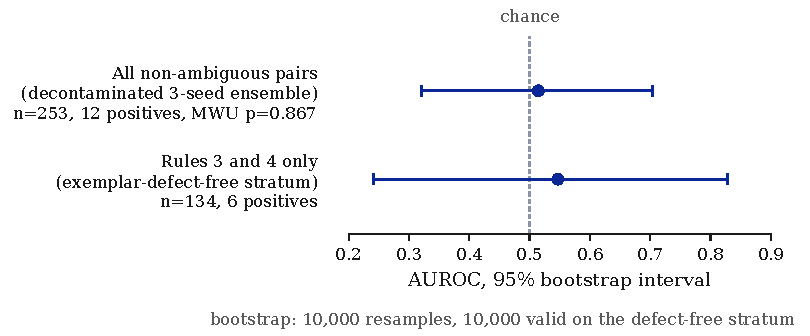
\includegraphics[width=0.92\linewidth]{figures/fig-disc-strata.pdf}
\caption{The measurement that closes the largest objection to
Chapter~\ref{ch:eval}. On the strata where the annotated evidence is correct by
construction, the detector's ranking is at chance rather than merely attenuated
toward it. The right panel rests on six positives and its interval is wide; the
claim it supports is that label contamination is not the explanation, not that
the true value is $0.5078$. Twenty of its $10{,}000$ resamples were dropped for
containing no positives, which is why the stratified band is shown alongside.}
\label{fig:disc-strata}
\end{figure}

\begin{figure}[t]
\centering
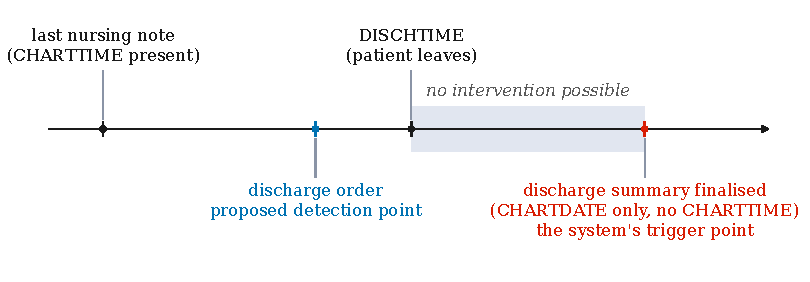
\includegraphics[width=0.92\linewidth]{figures/fig-disc-actionability.pdf}
\caption{The actionability flaw. The document that supplies one half of the
comparison does not exist until after the patient has left, so the prevention
story the design assumed is unavailable from this trigger. Either detection
moves to the discharge order, or the contribution is retrospective audit.}
\label{fig:disc-actionability}
\end{figure}

\section{Summary}
\label{sec:disc-summary}

Of the four research questions, one is answered negatively with a mechanism
(weak supervision cannot replace expert annotation here, because the labeller's
marginal is inverted by roughly $21\times$ and the student inherits it), one is
unaddressable in this resource (temporal ordering, because \texttt{CHARTTIME} is
null for every discharge summary), and two were never tested (authority
conditioning, whose parameter was initialised at the values reported as
discovered and sits where a normalisation erases it; and severity ranking, whose
component received no gradient).

The limitations are severe and are stated as such. $299$ annotated pairs against
a stated requirement of $548$. One annotator with no established inter-rater
reliability and a previously reported $\kappa$ of $1.000$ that is circular and
retracted. An exemplar selection defect affecting $41.4\%$ of action-conflict
candidates, which makes the measured $4.0\%$ precision an upper bound on
annotation validity rather than an estimate of pool quality. One institution, one
era, one primary cohort, retrospective throughout. No sub-day temporal ordering.
And a detection point that cannot precede the patient's departure, which is a
design flaw rather than a caveat and which forces a choice between moving
detection to the discharge order and reframing the contribution as retrospective
audit.

The central finding survives the most serious of these. On Rules 3 and 4, which
cannot exhibit the exemplar defect, the detector's AUROC is $0.5078$ with
Mann-Whitney $p = 0.953$ and a bootstrap $95\%$ interval of $[0.2217, 0.7615]$,
$[0.2643, 0.7344]$ when stratified. Six positives support that estimate, $20$ of
its $10{,}000$ resamples had to be discarded for containing none of them, and
both facts are stated rather than absorbed. It also survives a defect in the
reporting itself: the figures this thesis previously gave for the detector were
the contaminated configuration's, and the decontaminated retrain that replaces
them is worse on recall, precision, $F_1$ and $\kappa$.

The work that follows should start upstream of everything this project spent its
effort on: a better candidate generator, because $4.0\%$ precision is the binding
constraint and no downstream model repairs it; a weak labeller with a validated
operating point, or none; re-annotation of the $739$ candidates whose evidence
changed; a second annotator; and a second institution.

% ============================================================================
%  Chapter 10. Conclusion
%
%  \input file. Requires natbib in the parent preamble.
%  Bibliography: accord/thesis/refs.bib
%
%  Short by design. Every number restated here is derived in Chapters 3 to 9.
%  No new claim, no new number.
% ============================================================================

\chapter{Conclusion}
\label{ch:conclusion}

\section{What Was Asked}
\label{sec:conc-asked}

A patient on eleven medications is discharged. A nursing note records that the
loop diuretic was held because the patient had become hypovolemic. The discharge
summary instructs that it be continued at the admission dose. The two documents
disagree, only one of them governs what happens next, and it is not the one
containing the reason the instruction is wrong.

This thesis asked whether that disagreement can be detected automatically. It
posed four questions: whether conditioning on note-type authority beats
symmetric inference, whether temporal metadata helps, whether published
guidelines can rank confirmed contradictions by danger, and whether weak
supervision from a language model can replace expert annotation at the scale a
detector requires. It built the pipeline the field would naturally build to
answer them: rule-based candidate mining, language model weak supervision, and a
purpose-built neural detector over a domain-pretrained clinical encoder.

\section{What Was Found}
\label{sec:conc-found}

The clinical problem is real. Four transparent rules over one institution's notes
surface $1{,}978$ candidates across $1{,}203$ admissions from a heart-failure
cohort of $9{,}783$, and a board-certified pharmacist confirms $12$ genuine
contradictions in a $299$-pair stratified sample, four of them rated $4$ or $5$
for danger. That is systematic, not anecdotal.

The pipeline fails at every stage.

Candidate mining enriches the pool to a $4.0\%$ base rate, which is a real gain
over an unfiltered background rate orders of magnitude lower, but it attaches
the wrong evidence to $41.4\%$ of action-conflict candidates, because the trigger
quantified over sets of medication mentions while the exemplar selector indexed
positionally, and because no field existed upstream in which the distinction
could be expressed. The annotator, the weak labeller, and the model all reasoned
about that evidence.

Weak supervision fails on calibration rather than on comprehension. The labeller
assigned the positive class to $84.9\%$ of $1{,}679$ candidates against a $4.0\%$
measured base rate, so at least $95\%$ of its positive labels are wrong. The
student then reproduced the teacher's per-rule predicted-positive rate to within
$1.5$ percentage points on three of four rules, while the true prevalences on
those rules differ by more than a factor of four, and on the one rule where the
teacher was genuinely selective the student regressed to its own prior instead
of inheriting the distinction.

Three architectural contributions do not survive an audit of the code that
produced their numbers. The authority parameter reported as discovered at
$(0.5, 1.0)$ was initialised at exactly $[0.5, 1.0]$, moved by $1.8\%$ and
$0.6\%$, sits on a branch a subsequent normalisation largely erases, and is
outperformed by the symmetric variant on both reported metrics. The auxiliary
rule head's $F_1$ of $0.9603$ is a copy of an input feature and collapses to
$0.0654$ and $0.0595$ on two transfer cohorts. The severity component has no
guideline corpus, receives no gradient, and emits scores spanning $0.398$ to
$0.610$, the range of an untrained sigmoid.

The detector has no rank signal. On the $299$ annotated pairs its AUROC is
$0.460$, with average precision at the no-skill line, Mann-Whitney $p = 0.64$,
and a bootstrap $95\%$ interval of $[0.287, 0.633]$; its fifteen highest-scored
pairs contain zero true contradictions; and at every threshold from $0.05$ to
$0.15$ its predicted-positive rate is exactly $1.000$. Restricted to the strata
that cannot exhibit the exemplar defect, AUROC is $0.5078$ with Mann-Whitney
$p = 0.953$, on six positives. Its Matthews correlation is $-0.007$; the
labeller it was distilled from scores $-0.044$. A general-purpose model prompted
zero-shot on the same evidence, with no training and no clinical components, is
the only system in the comparison above chance.

Of the four questions: RQ4 is answered negatively with a mechanism; RQ2 is
unaddressable in MIMIC-III, because \texttt{CHARTTIME} is null for every
discharge summary; and RQ1 and RQ3 were never tested, because in each case the
component that would have answered them could not have produced an informative
answer under any data.

\section{What It Means for Anyone Attempting This}
\label{sec:conc-means}

Three statements are worth carrying out of this document.

\paragraph{The binding constraint is upstream of the model.} A candidate pool at
$4.0\%$ precision determines what every downstream stage can achieve, and no
detector in this thesis adds lift over the rule that generated its candidates:
precision tracks each rule's base rate to within a tenth of a percentage point,
and on the one rule where the model exercises selectivity it selects wrongly.
Effort spent on architecture was effort spent on the wrong stage. Anyone
building this system should spend it on extraction, on evidence attribution, and
on candidate generation, and should validate each against human annotation
before a model exists.

\paragraph{The task is not the problem.} A zero-shot general-purpose model, on
the same $299$ pairs, with the same evidence, reaches $8.45\%$ precision at
$50\%$ recall with a positive Matthews correlation. That is not a usable
clinical system, and it should not be presented as one: eleven false alarms per
true contradiction, half the contradictions missed. But it is above chance,
which means the evidence contains extractable signal and the failure documented
here belongs to this pipeline rather than to the problem. Every hypothesis this
thesis set out to test remains open.

\paragraph{The intended intervention point does not exist.} The system is
triggered by the discharge summary, and the discharge summary is a retrospective
document that frequently is not finalised until the patient has gone. No alert
built on this trigger can prevent anything. Either detection moves to the
discharge order, which changes the task from cross-note textual inference toward
reconciliation against a structured order set, or the contribution is
retrospective audit and quality assurance and should be described that way. That
question should be settled before any of the modelling work is repeated.

\section{The Transferable Lesson}
\label{sec:conc-lesson}

The most durable result in this thesis is methodological, and it is not about
contradictions.

A system can produce a plausible headline number while every component that
supposedly produces it is either untrained, leaking, or reading the wrong
evidence. This one did. It reported a contradiction $F_1$, an auxiliary-task
$F_1$ of $0.9603$, an authority hierarchy described as discovered, a severity
score, an ablation table with error bars, and a $\kappa$ of $1.000$ offered as
evidence of annotation reliability. Behind those numbers: a parameter that never
moved from its initialisation, an auxiliary label written into the model's own
input, two output heads absent from the loss, a standard deviation over two
seeds plus a pasted literal compared against a reference row that the ablation
script does not run, and an agreement statistic between two quantities standing
in an identity relation. Every one of these passed internal review. None of them
survives its own first diagnostic.

The diagnostics are not sophisticated. Print a module manifest at training time
with parameter counts and loss-graph membership. Log
$\lVert\theta_{\text{final}} - \theta_{\text{init}}\rVert /
\lVert\theta_{\text{init}}\rVert$ for any parameter reported as learned. Assert
that an auxiliary head's target is not derivable from its inputs, and check by
transfer rather than by held-out accuracy. Report a majority-class baseline
beside every $F_1$. Print the number of distinct values a confidence field takes.
Print the empirical range of every score the model emits. Estimate the base rate
on a human-labelled sample \emph{before} generating weak labels, and print the
labeller's marginal against it. Assert group disjointness of splits, and assert
that the evaluation set is absent from training, by identifier, at load time.

None of these is novel. All of them are omitted routinely, including here. What
this thesis contributes is the demonstration that their absence is not a hygiene
issue but a load-bearing one: it is what allowed four unsupported claims to
reach a submission, and it is the reason a system with no measurable
discriminative ability could be described, in good faith, as working.

The corollary is uncomfortable and is the reason this document exists in its
present form. The failures documented here were not found by peer review, by a
held-out set, or by a novel evaluation. They were found by an adversarial audit
of the project's own code against the project's own claims, conducted after the
results were in. A pipeline that runs end to end, produces numbers, and is never
compared against its own specification will report the specification. Only
deliberate self-falsification surfaces the difference, and the discipline that
makes it routine is the thing this field is missing more than it is missing
another architecture.

\section{Closing}
\label{sec:conc-closing}

Dangerous medication contradictions between nursing notes and discharge
summaries are real, recurring, and worth detecting. The pipeline the field would
naturally build for them fails at every stage. The failures are independent of
one another, each has an identifiable mechanism, each has a detector costing a
few lines of code, and none of them was found until the project set out to
falsify itself.

That is the contribution. It is a negative result, it is measured four
independent ways, and it is offered so that the next attempt starts further
along than this one did.


\backmatter
\bibliographystyle{plainnat}
\bibliography{refs}

\end{document}
